\documentclass[a4paper,12pt]{article}

% ================== Packages ==================
\usepackage[utf8]{inputenc}   % 中文注释无妨
\usepackage[T1]{fontenc}
\usepackage{geometry}
\geometry{margin=1in}
\usepackage{setspace}
\setstretch{1.5}
\usepackage{amsmath,amssymb}
\usepackage{graphicx}
\usepackage{booktabs,multirow,makecell}
\usepackage{arydshln,adjustbox}
\usepackage{float}
\usepackage{hyperref}
\usepackage{pifont}
\usepackage{orcidlink}
\usepackage{xcolor}
\usepackage{caption}
\usepackage{subcaption}
\usepackage{enumitem}
\usepackage{todonotes} % 仅写中文注释 \todo{}
\usepackage{adjustbox}
\usepackage{amsmath} 
\usepackage{amssymb}
\usepackage{mathtools}
\usepackage{multirow}
\usepackage{bm}
\usepackage{booktabs}
\setlength{\aboverulesep}{1pt}
\setlength{\belowrulesep}{1pt}
\setlength{\cmidrulekern}{1pt} % \cmidrule 两端也更贴


% ================== Meta ==================
\newcommand{\Title}{3D Human Motion Generation Using Multimodal Approaches}
\newcommand{\AuthorName}{Tengjiao Sun}
\newcommand{\Supervisors}{Dr. Hansung Kim, Dr. Zhiwu Huang}
\newcommand{\Degree}{18-Month Doctoral Report}
\newcommand{\Affil}{University of Southampton\\Faculty of Engineering and Physical Sciences\\Electronics and Computer Science}
\newcommand{\DateSubmitted}{\today} % TODO: 如需固定日期可改为具体日期




% ================== Document ==================
\begin{document}
\onecolumn

\numberwithin{table}{section}
\numberwithin{figure}{section}
\numberwithin{equation}{section}

% ---------- Title Page ----------
\begin{titlepage}
    \centering
    \vspace*{2cm}
    {\LARGE \textbf{\Affil}}\\[1.2cm]
    {\Huge \textbf{\Title}}\\[0.8cm]
    \rule{\textwidth}{0.5pt}\\[0.4cm]
    {\large \textbf{Author:} \AuthorName}\\[0.2cm]
    {\large \textbf{Supervisors:} \Supervisors}\\[1.4cm]
    {\large \Degree}\\[0.2cm]
    {\large \DateSubmitted}\\[1.2cm]
\end{titlepage}

% ---------- Abstract ----------
\begin{abstract}
% TODO(中文注释)：150–250词。简述研究动机（跨模态语义对齐、可控性/编辑、长时序）、9个月阶段核心（MCRE），本阶段新增（video priors；hierarchical AR for infinite-length），并点出主要实验结论与意义。
\end{abstract}

\tableofcontents
\newpage

% =========================================================
% 1. Introduction
% =========================================================
\section{Introduction}
\subsection{Background and Motivation}
% 注：过去9个月未涉及 Flow Matching；未实现控制/编辑功能，以下仅描述表征对齐与设计意图。

Human motion generation underpins a wide range of applications in virtual/augmented reality, character animation for games and film, human–robot interaction, and telepresence. Among possible interfaces, \emph{text} stands out as a natural and lightweight modality for specifying high-level intent, compositional constraints, and scene context. This has driven a shift from handcrafted controllers to data-driven, generative models that map free-form descriptions to plausible, temporally coherent 3D motions \cite{ahuja2019language2pose,petrovich2022temos,kim2023flame,tevet2022human}.

Despite visible progress, translating open-ended language into continuous human movement remains fundamentally challenging. First, there is a representation gap: textual semantics are symbolic and sparse, whereas motion is high-dimensional, continuous, and governed by kinematic and physical constraints. Bridging this gap requires models that learn aligned cross-modal representations while remaining sensitive to local limb dynamics, contacts, and global trajectory structure. Second, there is a control gap: practical systems ultimately need not only one-shot generation from text, but also editing, composition (combining multiple intents), and conditioning on auxiliary signals such as reference motion or video. Third, there is a horizon gap: many applications demand real-time interaction and long-horizon behaviors with stable continuation, re-prompting, and style persistence, where error accumulation and distribution drift are common failure modes.

Methodologically, existing families offer complementary strengths and weaknesses. Variational Autoencoder(VAE) approaches provide fast inference and broad coverage but may sacrifice fine detail and control \cite{kingma2013auto,petrovich2022temos}. Tokenization-based methods discretize motion into codebooks and leverage transformers for powerful sequence modeling, yet can suffer from discretization artifacts and autoregressive exposure bias on long sequences \cite{zhang2023generating,jiang2024motiongpt}. Diffusion models operate in continuous spaces and set a high bar for fidelity and diversity, but are often optimized for single-task text-to-motion and can be computationally heavy at inference time \cite{sohl2015deep,tevet2022human,chen2023executing,zhang2024motiondiffuse}. These trade-offs motivate hybrid designs that retain diffusion-level quality while enabling low-latency control and long-horizon stability.

A promising direction is to enrich conditioning beyond text. Motion capture snippets, 2D video priors, and learned adapters can inject stronger temporal and structural cues, improving both semantic alignment and local realism. During the first nine months I focused on representation: I unified text and motion conditions in a shared space by training a lightweight motion adapter aligned to a pre-trained text encoder (for example, CLIP~\cite{radford2021learning}). This shared space is designed to admit linear editing directions and multi-condition composition in principle.

Two open problems remain for a practical system: (i) scaling multimodal conditioning to richer priors such as short reference videos without substantial computational overhead, and (ii) maintaining interactive, infinite-length generation with robust continuation, prompt switching, and style consistency. Addressing these requires stronger yet lightweight fusion mechanisms that leverage video priors during training and inference, and architectures that combine the streaming advantages of autoregression with the refinement strengths of diffusion. This report centers on these two axes, laying the groundwork for controllable, generalizable, and efficient text-to-motion systems across generation, (future) editing, and long-horizon continuation under a unified multimodal framework.



% 结尾功能：引出“视频先验的轻量融合”与“AR+diffusion 的互补”两条主线（不提FM）。

% \subsection{Research Questions and Scope}
% % TODO：列出 3–4 个研究问题（统一条件表征；2D视频先验如何迁移到3D动作；低延迟长时序；多任务/多模态可编辑性）。
% % 写作意图：将研究问题收束为可评估的目标；范围界定清晰，便于后续方法与实验对齐。

% This project investigates how to move from text-only motion generation toward a unified multimodal framework with stronger priors and longer horizons, while keeping inference practical. We formulate the agenda around the following questions.

% \begin{enumerate}[leftmargin=1.2em,label=(RQ\arabic*)]
%     \item How can we construct a shared conditional space for text, motion snippets, and short reference videos that preserves semantic alignment and temporal structure, admits linear composition, and degrades gracefully to text-only input when auxiliary modalities are absent?
%     \item Which lightweight fusion mechanisms best exploit video priors during training and inference while keeping computational overhead small, and how should modality weights or perturbations be scheduled to remain robust under domain shift and missing modalities?
%     \item How can we enable interactive, infinite-length generation with stable continuation and prompt switching, minimizing drift and exposure bias over long horizons under realistic latency constraints?

% \end{enumerate}

% \paragraph{Scope}
% % 注：明确“做什么/不做什么”，避免评审误解。

% \textit{Problem setting.} Inputs include a text prompt and, optionally, a short motion snippet or a short reference video; outputs are 3D human motions represented as pose sequences on a standard skeletal topology. Single-person motions are considered; multi-person interaction is out of scope for this stage.

% \textit{Datasets and benchmarks.} We focus on HumanML3D and a curated subset of Motion-X for language–motion alignment, and derive video priors where applicable. All comparisons use fixed splits and identical preprocessing; additional dataset statistics and cleaning rules will be reported in the appendix.

% \textit{Metrics.} We report distributional distance (FID-style on motion features), retrieval precision (Top-1/2/3), MM-Dist, diversity, and an editing/style consistency score such as MEC. Long-horizon stability is quantified by drift and contact slippage indicators, and by velocity/acceleration distribution consistency. Runtime and per-frame latency are included for streaming scenarios.

\subsection{Multimodal Motion Generation with MotionDirector}
Building on this foundation, the first major line of work is \textbf{MotionDirector}, a diffusion-based multimodal framework that emphasizes controllability and expressiveness under joint textual and visual conditioning. Text provides high-level semantic intent, but often lacks temporal precision; video, conversely, offers temporally coherent demonstrations but requires acquisition and limits generalization. MotionDirector is inspired by the concept of theatrical direction, where both verbal instructions and visual demonstrations jointly guide a performance. 

MotionDirector adopts a dual-conditioning paradigm, with two complementary modules:  
\begin{itemize}
    \item \textbf{DUET (Dual-stream Unified Encoding and Transformation):} a plug-and-play cross-modal fusion mechanism that injects video-grounded cues into motion representations through a unified encoding pathway and dynamic attention, thereby improving temporal fidelity and semantic grounding.  
    \item \textbf{DASH Loss (Distribution-Aware Structural Harmonization):} a distribution-level alignment objective that narrows the gap between synthesized motion features and real video-grounded representations, stabilizing training and accelerating convergence.  
\end{itemize}
In addition, MotionDirector introduces an \textbf{auto-guidance mechanism}~\cite{karras2024guiding}, which leverages a degraded version of the model itself to adaptively balance text and video conditions without requiring an external unconditional branch. This design enables stronger conditioning, more faithful semantics, and greater controllability, while maintaining diversity. Taken together, these components allow MotionDirector to produce expressive and controllable motions that are both semantically consistent and visually realistic, advancing the state of the art in multimodal diffusion-based generation.

\subsection{Efficient and Scalable Generation with MOGO}
While MotionDirector addresses controllability and multimodal grounding, diffusion inherently incurs high inference latency due to its iterative sampling. To support real-time and interactive scenarios, efficiency and scalability must also be prioritized. To this end, the second major line of work is \textbf{MOGO (Motion Generation with One-pass)}, an autoregressive framework that emphasizes low-latency decoding and infinite-length scalability.  

MOGO consists of two key innovations:  
\begin{itemize}
    \item \textbf{MoSA-VQ (Motion Scale-Adaptive Residual Vector Quantization):} a hierarchical tokenization module that introduces learnable scaling and cross-level decorrelation, yielding compact and disentangled motion codes while improving codebook utilization.  
    \item \textbf{RQHC-Transformer (Residual Quantized Hierarchical Causal Transformer):} an autoregressive decoder aligned with the quantization hierarchy, capable of generating all motion tokens in a \emph{single forward pass}. This one-pass decoding ensures temporally coherent synthesis while drastically reducing inference latency.  
\end{itemize}

Moreover, MOGO supports \textbf{infinite-length generation} by seamlessly extending motions autoregressively, with the flexibility to incorporate new textual prompts at arbitrary points in time. This property makes it well-suited for interactive applications such as avatar control or robot teleoperation. To enhance robustness under real-world prompts, MOGO further integrates a \textbf{Textual Condition Alignment (TCA)} module, which leverages large language models with Chain-of-Thought reasoning to normalize free-form user inputs into structured, executable motion instructions. This substantially improves both zero-shot generalization and semantic fidelity.



\subsection{Contributions at 18 Months}
% TODO：以要点总结当前阶段贡献；建议与后文章节对齐。
\begin{itemize}[leftmargin=1.2em]
    \item A unified conditional representation and editing framework (MCRE) for text \& motion with linearized semantic editing in the shared space.
    \item Video-prior enhanced generation and editing with lightweight multimodal fusion, plus automated video-data cleaning.
    \item A hierarchical, one-pass autoregressive design enabling near real-time, infinite-length generation and prompt switching.
\end{itemize}

\noindent Publications to date and in preparation include:
\begin{itemize}
    \item \textit{MCRE: Multimodal Conditional Representation and Editing for Text-Motion Generation}, accepted at ECCV Workshop on Foundation Models for 3D Humans.
    \item \textit{Hi-RQCT: Hierarchical Residual-Quantized Causal Transformer for High-Quality 3D Human Motion Generation}, accepted at CVMP 2025, extending the RQHC-Transformer design.
    \item \textit{MOGO: Residual Quantized Hierarchical Causal Transformer for Real-Time and Infinite-Length 3D Human Motion Generation}, currently under second-round review at AAAI 2026.
    \item \textit{MotionDirector: Directing Motion with Video Cues}, planned submission to CVPR 2026.
\end{itemize}


\newpage

% =========================================================
% 2. Related Work
% =========================================================
\section{Related Work}

\subsection{Text-to-Motion: VAEs, Tokenization, Diffusion}
% 写作意图：概述三条主流技术线的代表方法、优势/局限与演进趋势；与后文方法动机衔接；仅引用有代表性的工作。

Research on text-conditioned motion has converged on three major families: variational autoencoders, tokenization-based transformers, and diffusion models. Each family makes a distinct trade-off between fidelity, controllability, and efficiency.
\begin{figure}[t]
    \centering
    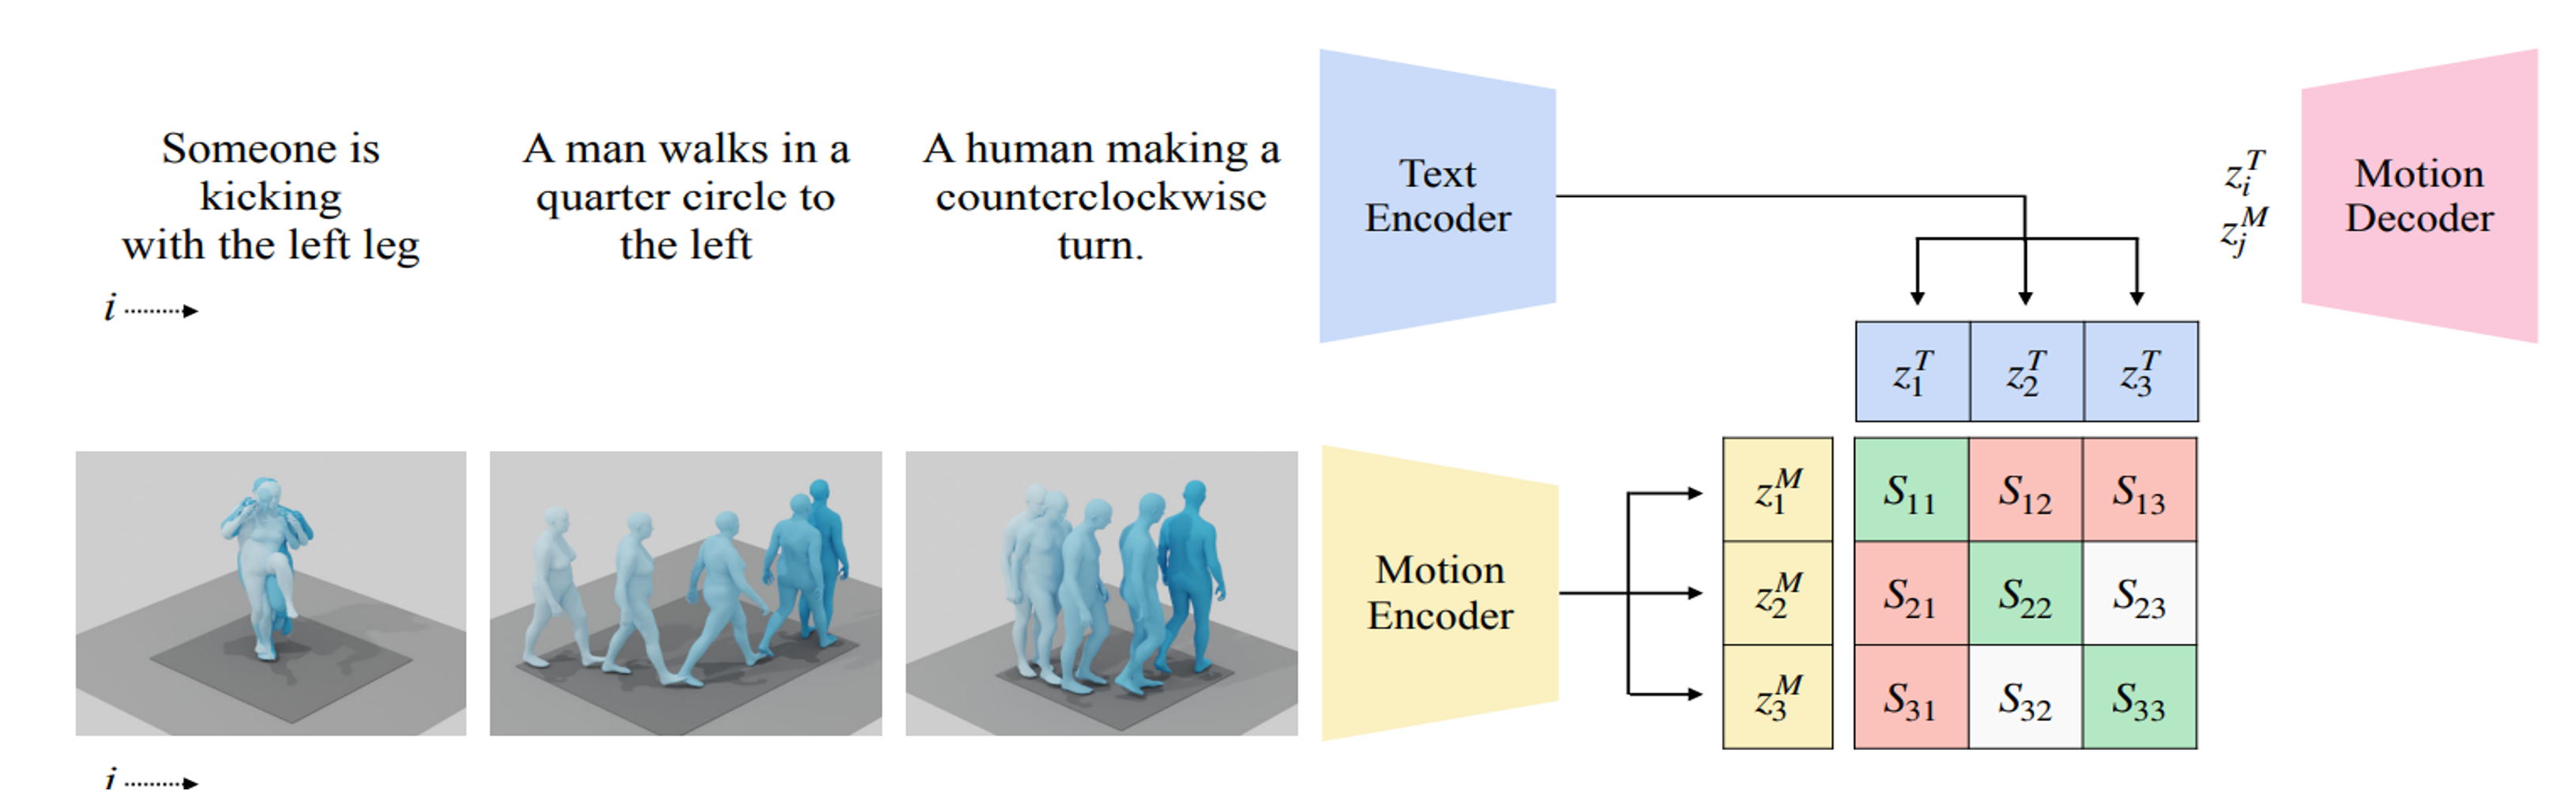
\includegraphics[width=\textwidth]{figs/TMR.png}
    \caption{TMR: Text-to-Motion Retrieval Using Contrastive 3D Human Motion Synthesis\cite{petrovich2023tmr}}
    \label{fig:TMR}
\end{figure}


\paragraph{VAEs}
VAE-based approaches encode motions into a continuous latent space and decode conditioned on text, yielding fast amortized inference and broad coverage \cite{kingma2013auto}. TEMOS learns a text–motion latent alignment that supports generation from language descriptions \cite{petrovich2022temos}, while TMR, as shown in Fig.~\ref{fig:TMR}, couples contrastive retrieval with generative synthesis to improve language–motion compatibility \cite{petrovich2023tmr}. These methods are attractive for their training stability and runtime speed, but they can underfit fine-grained temporal structure and contact dynamics; posterior collapse and over-smoothing remain common concerns, especially for long or compositionally complex prompts.


\begin{figure}[t]
    \centering
    \includegraphics[width=\textwidth]{figs/MDM.png}
    \caption{MDM: Motion Diffusion Model for text-to-motion generation\cite{tevet2022human}.}
    \label{fig:MDM}
\end{figure}

\paragraph{Diffusion models.}
Diffusion operates directly in continuous spaces and has set high bars for fidelity and diversity across modalities \cite{sohl2015deep}.  As shown in Fig.~\ref{fig:MDM}, MDM conditions a denoising process on text features to synthesize temporally coherent poses \cite{tevet2022human}. MotionDiffuse extends conditional mechanisms for text-to-motion with improved sampling \cite{zhang2024motiondiffuse}. Latent-diffusion variants map motions to compact feature spaces before denoising, improving efficiency without sacrificing quality \cite{chen2023executing}. Despite these advances, diffusion pipelines are often tuned for single-task text-to-motion and can be computationally heavy at inference time; step counts, guidance scales, and noise schedules must be balanced against latency, which complicates interactive use and very long sequences.

% \paragraph{Representation Learning}
% Motion representations are typically based on either SMPL~\cite{cai2024smpler} parameters or hand-crafted features. The SMPL-based approach models motion by manipulating pose and shape parameters to generate 3D human meshes~\cite{cai2024smpler,loper2023smpl,wang2024disentangled,cao2023sesdf}. Alternatively, hand-crafted features~\cite{guo2022generating,starke2022deepphase,chen2023executing} are designed to address animation artifacts like foot sliding, improving realism and control in motion synthesis.


\paragraph{Multimodal Condition}
Adapters, controllers, and classifier-free guidance (CFG) are widely used to enhance multimodal generative models. In Fig.~\ref{fig:motion_adapter}, MCRE~\cite{sun2024mcre} enable efficient modality adaptation (e.g., text-to-motion) via lightweight modules in CLIP space. Controllers improve controllability without additional parameters, as demonstrated in TLControl~\cite{wan2024tlcontrol}. CFG~\cite{shen2024rethinking,kwon2025tcfg} guides diffusion models toward high-quality conditional generation, especially in text-to-image tasks. Together, these mechanisms significantly improve flexibility and generation quality in multimodal settings.



\paragraph{Tokenization and autoregressive transformers.}
\begin{figure}[t]
    \centering
    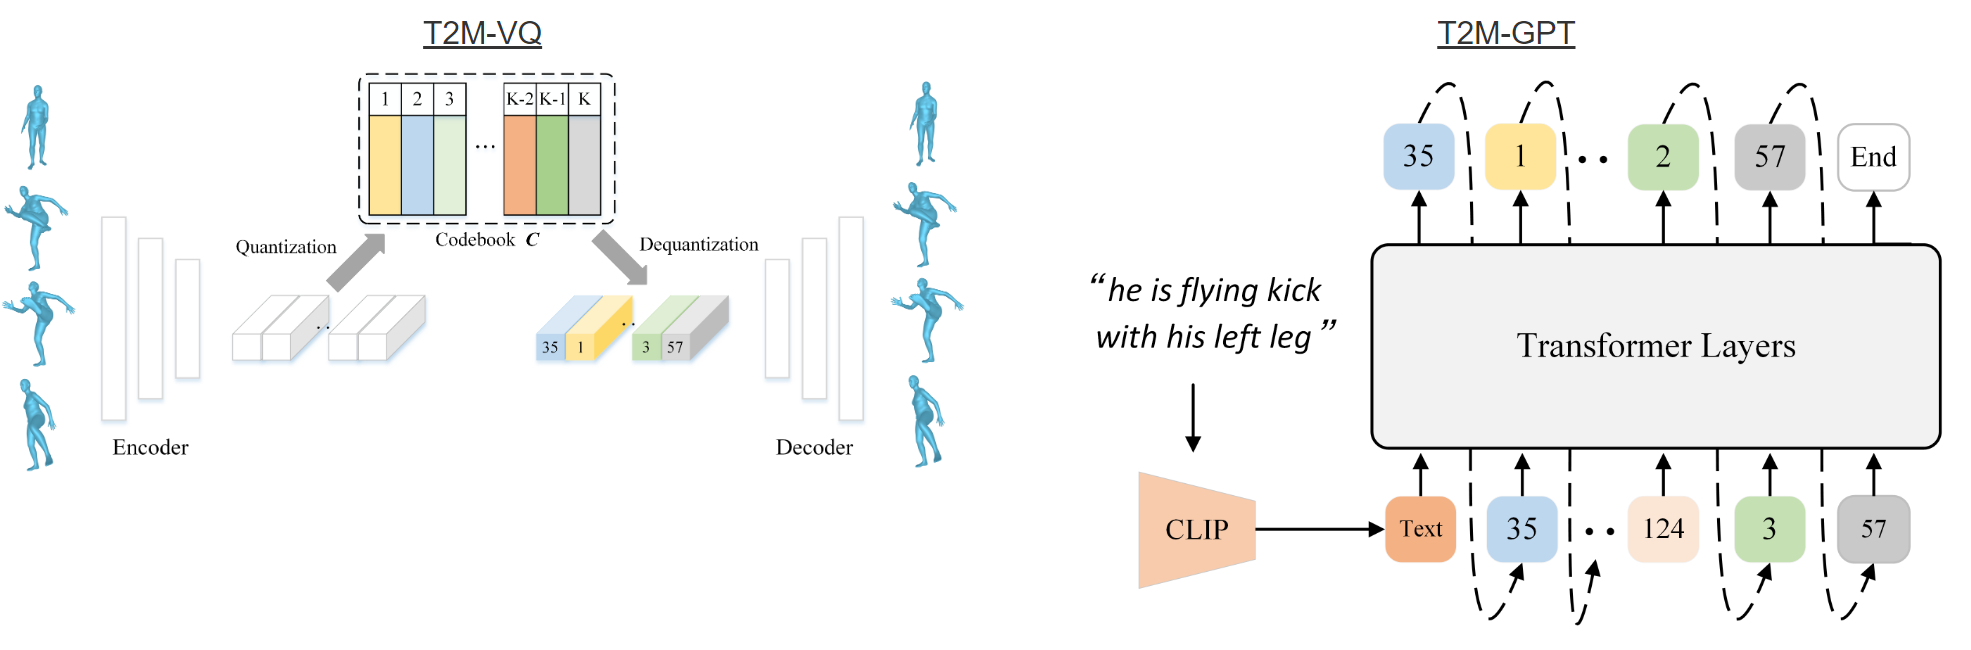
\includegraphics[width=\textwidth]{figs/T2M-GPT.png}
    \caption{T2M-GPT: Text-to-Motion Generation using Transformer-based Language Models\cite{zhang2023generating}.}
    \label{fig:T2M-GPT}
\end{figure}

Discretizing continuous motion data into tokens via vector quantization is central to transformer-based motion generation. TM2T~\cite{chuan2022tm2t} introduced VQ-VAE to map motions to discrete sequences. As shown in Fig.~\ref{fig:T2M-GPT}, T2M-GPT~\cite{zhang2023generating} enhanced token quality with exponential moving average and codebook reset techniques. AttT2M~\cite{zhong2023attt2m} improved quantization through body-part-aware encoding. MoMask~\cite{guo2024momask} advanced this with residual vector quantization (RVQ), producing multi-level tokens for better reconstruction quality. Compared to prior work, our approach introduces learnable feature scaling into the residual vector quantization process, allowing each quantization level to adaptively adjust the magnitude of its residuals. This scaled RVQ mechanism stabilizes the residual distribution across quantization stages, mitigates the risk of later stages collapsing to noise, and ensures more effective codebook utilization. As a result, the model benefits from improved reconstruction fidelity, better token expressiveness, and enhanced training stability. 



\paragraph{Summary}
In short, VAEs offer speed but may lose detail; tokenization-based transformers offer strong sequence modeling but face discretization and long-horizon drift; diffusion offers the best perceptual quality but at higher inference cost and with limited multimodal control in standard forms. These complementary strengths motivate hybrid and multimodal designs that retain diffusion-level fidelity while improving controllability and long-horizon practicality, which is the direction pursued in this report.
% 衔接语：为后续的视频先验融合与长时序/交互式生成架构埋下动机。


\subsection{Adapters and Multimodal Control}
% 写作意图：综述“在不大改基础模型的情况下提升可控性”的Adapter范式；覆盖注入位置、训练方式与权衡；将图像/视频领域做法映射到动作生成，并交代本工作采用的对齐式思路（但不声称已实现控制）。

Adapters provide a practical route to controllable generation by attaching small trainable modules to a large frozen backbone. The core idea is to expose conditioning signals—text, images, videos, or motion snippets—through lightweight pathways that modulate intermediate features without retraining the entire model. This yields fast iteration, parameter efficiency, and the ability to stack multiple controls.

A common pattern is decoupled cross-attention, where a separate conditioning encoder produces keys and values that feed cross-attention blocks alongside text tokens. IP-Adapter follows this idea to inject image prompts while preserving the underlying text pathway, enabling style and content control with little parameter overhead \cite{ye2023ip}. Another line adds a side branch that predicts residual feature maps aligned with the UNet hierarchy; ControlNet exemplifies this structure and has proven effective for structural constraints such as edges, depth, or keypoints \cite{zhang2023adding}. T2I-Adapter generalizes the side-branch idea into plug-and-play adapters that handle diverse cues (style, sketch, pose) across diffusion backbones \cite{mou2024t2i}. In parallel, prompt-space editing methods like Prompt-to-Prompt operate at the embedding level, adjusting or mixing textual embeddings to manipulate content with minimal architectural changes \cite{hertz2022prompt}.

Beyond where to inject, training regimes influence stability and portability. Zero-initialized residual paths help preserve the base model at early stages; low-rank adaptation (LoRA)~\cite{hu2022lora} can replace or complement explicit adapters for parameter budget control; modality dropout during training improves robustness to missing or noisy conditions; and simple fusion rules (add, concat, hadamard) often compete surprisingly well with heavier attention blocks when the conditioning encoder is strong. These choices reflect a general design principle: keep the control path simple and predictable, and push semantic burden into the conditioning encoder and loss design.

Transferring these ideas to motion generation introduces additional constraints. Motion conditions carry temporal structure, contact patterns, and viewpoint ambiguities. A representation-lean approach is to align motion and text into a shared embedding space using a lightweight motion adapter trained against a frozen text encoder (e.g., CLIP). Once aligned, the generator can, in principle, accept either modality and combine them via simple fusion, while retaining a text-only fallback. This is the stance taken in our earlier representation work: I focused on learning a shared conditional space with a small transformer-based motion adapter aligned to text, deferring control and editing pipelines to future stages.

When the conditioning signal is a short reference video, adapters can serve as a vehicle to transport video priors into the motion backbone. Two practical options are: (i) a video-encoder branch that outputs per-frame or pooled tokens consumed by cross-attention in selected blocks; or (ii) a ControlNet-style~\cite{zhang2023adding} residual path attached at matching temporal resolutions. In both cases, modality-aware scheduling (weights for each condition, or perturbations such as dropout/noise applied to the control stream) helps avoid over-conditioning and improves generalization when the reference is weak or out of domain.

Finally, adapters interact with inference-time guidance. Classifier-free guidance remains the default for diffusion-style generators, but adapter pathways enable finer control by separating unconditional, text-only, and multimodal-conditioned passes. For interactive or streaming settings, lightweight adapters paired with caching-friendly architectures (autoregressive decoders or causal transformers) can amortize the cost of conditioning across long horizons, while retaining the option to disable or downweight auxiliary modalities on the fly. This combination—simple, modular injection plus robust scheduling—forms the basis of the multimodal control design used in this report’s subsequent methodology.
% 收束句功能：为后文方法里“简单融合头 + 共享条件空间 + 可拔插视频分支”的设计埋钩子，避免过度承诺控制已实现。



\subsection{Autoregressive Generation}
% 写作意图：回顾AR在线/低延迟优势与难点；结合离散化表示与分层建模的演进；为后文层级残差量化与因果Transformer铺垫。

Autoregressive (AR) models generate motion by predicting the next state conditioned on a causal history. Their main appeal is streaming capability and predictable latency: a decoder can emit frames or tokens as soon as context is available, making AR attractive for interactive or real-time use. When paired with attention mechanisms, AR models handle long-range dependencies, speaker intent changes, and prompt switching more naturally than single-shot decoders.

Early AR systems operated directly in continuous pose spaces, but suffered from compounding error and blurry dynamics on long horizons. Discretization via vector quantization reframed motion as a sequence modeling problem closer to language modeling \cite{zhang2023generating,jiang2024motiongpt}. By predicting code indices instead of raw poses, AR decoders benefit from robust token priors and efficient caching, and can reuse standard transformer tooling. However, exposure bias and quantization artifacts introduce drift and contact slippage over time, especially when contexts extend far beyond training lengths.

Recent work addresses these problems along two axes. The first axis concerns the representation: residual or multi-level quantization increases codebook capacity without exploding token rates, while regularizers that decorrelate levels reduce redundancy and stabilize training. Hierarchy also enables mixed rates, where slower-changing global trajectory tokens and faster local-kinematics tokens are modeled at different granularities, improving both efficiency and fidelity. The second axis concerns the decoder: causal transformers with relative position encodings and memory mechanisms maintain temporal coherence over long contexts; lightweight auxiliary losses on velocities, contacts, or short-horizon reconstructions mitigate drift; and scheduled prompting or periodic anchors reduce error accumulation during free-running generation. Additionally, With appropriate conditioning interfaces, AR decoders support mid-sequence prompt edits and content injection, which are difficult to realize with pure denoising pipelines at similar speed.

In summary, AR generation provides a viable path to interactive and infinite-length motion, provided that the representation and the decoder are co-designed. Hierarchical residual quantization alleviates tokenization–fidelity trade-offs, and causal transformers with memory and lightweight regularization curb long-horizon drift. This review motivates the methodological choices that follow: a multi-level discrete representation coupled with a level-aligned causal transformer, designed for low-latency streaming while preserving semantic and kinematic coherence.
% 收束语：不宣称现阶段已实现所有能力，作为方法论动机与设计准则的铺垫。


% =========================================================
% 3. Methodology
% =========================================================
\section{Methodology}
\subsection{Recap: Multimodal Conditional Representation \& Editing (Months 0–9)}
% 写作意图：回顾 0–9 月阶段已完成的“统一条件表征”与对齐训练；强调设计初衷与离线可行性分析；不宣称已实现控制/编辑管线。

\paragraph{Design goal}
The objective was to establish a shared conditional space for text and motion such that semantically similar descriptions and motions map to nearby embeddings. This space is intended to support, in principle, linear composition and editing directions, while remaining compatible with diffusion-style generators used for text-to-motion.

\begin{figure}[t]
    \centering
    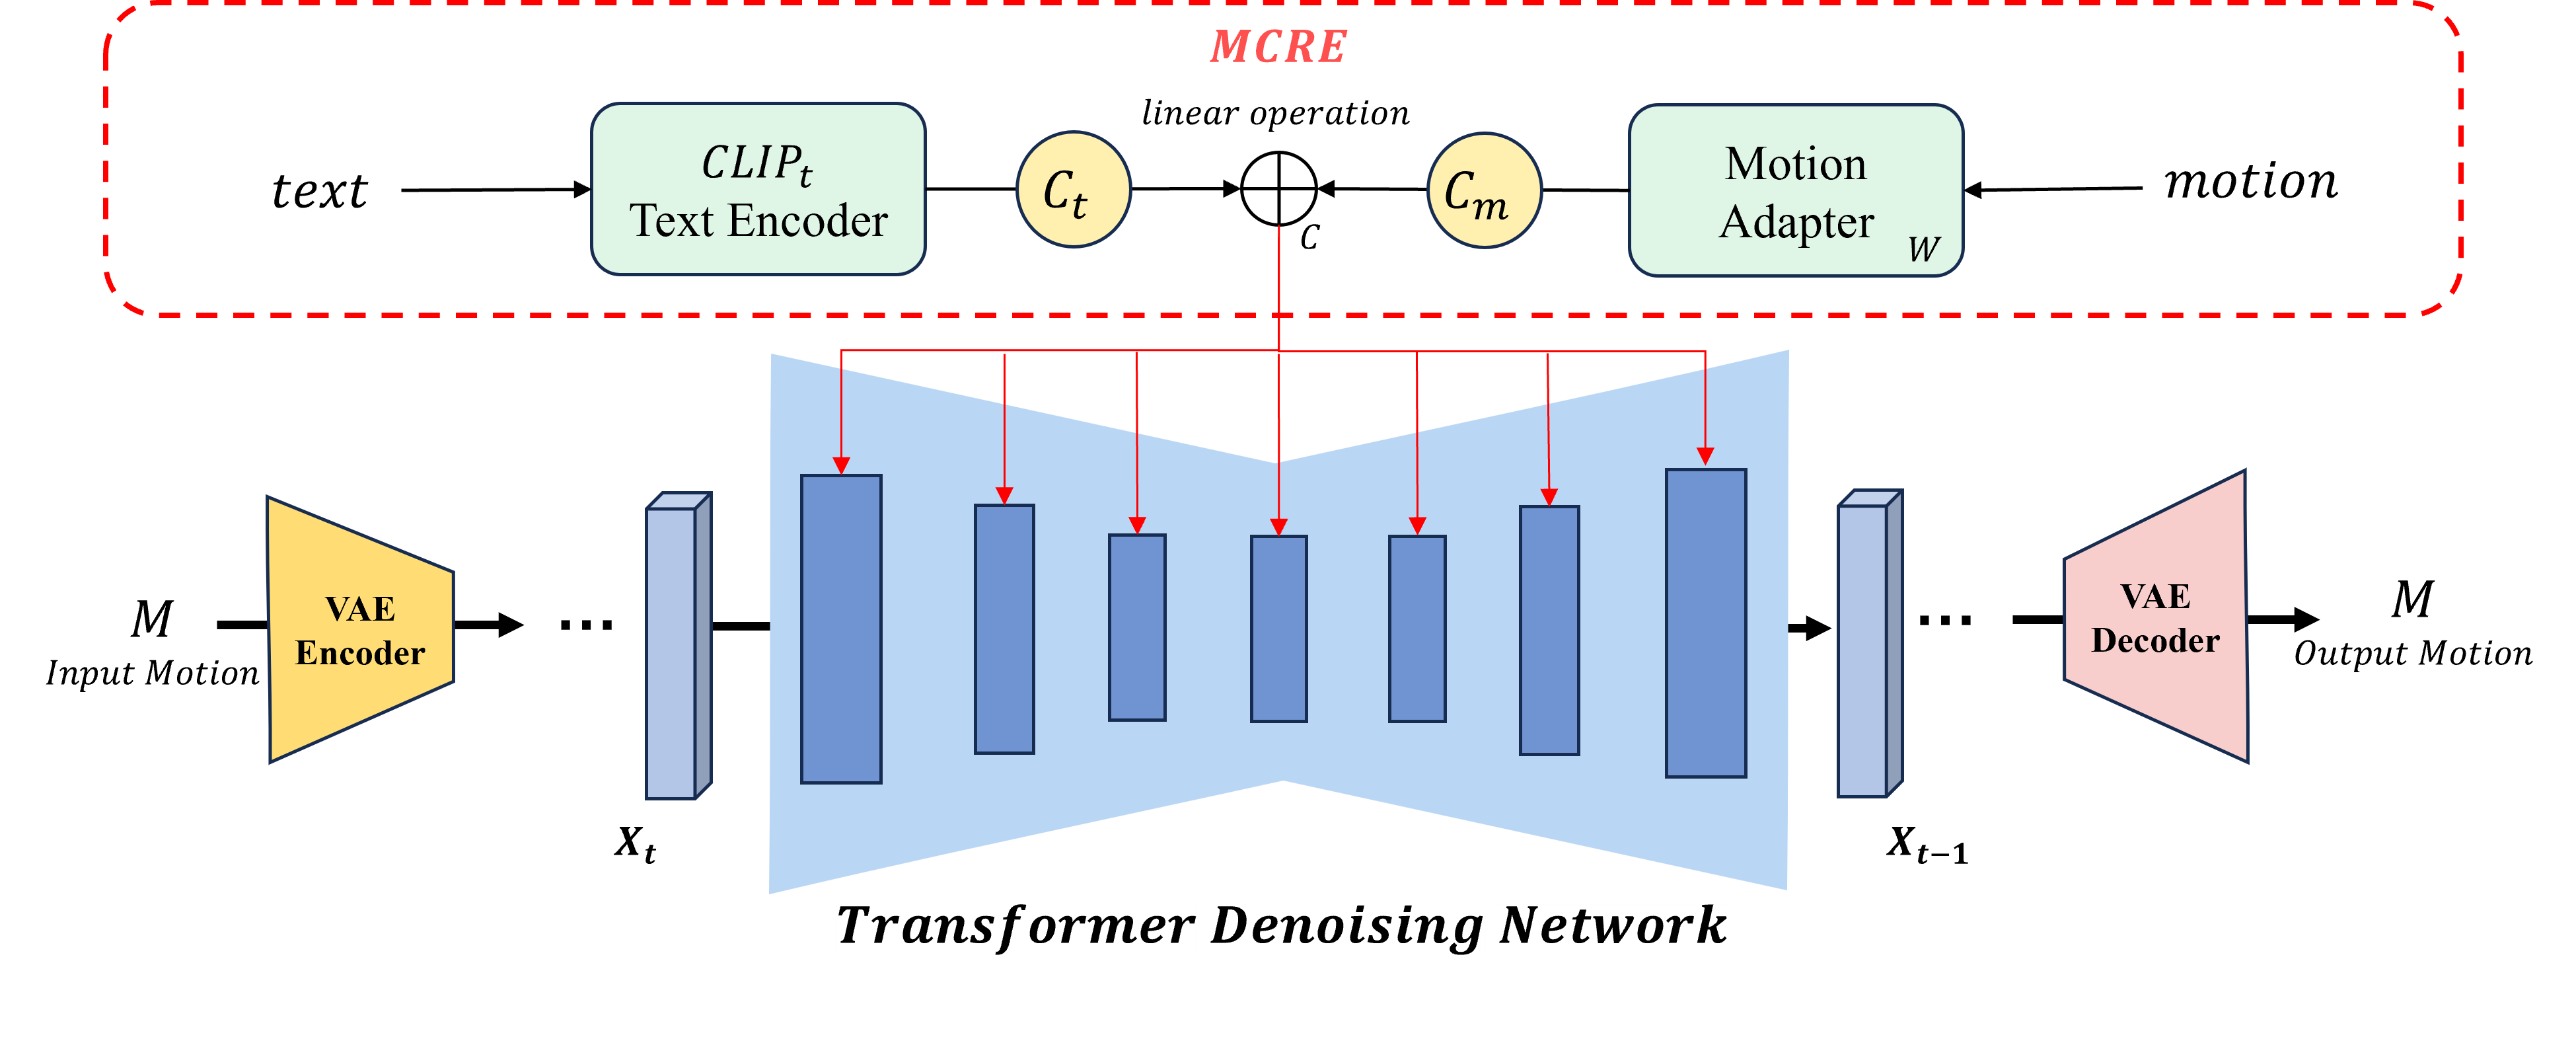
\includegraphics[width=\textwidth]{figs/whole_framework.png}
    \caption{Overview of the proposed MCRE framework for multimodal 3D motion generation.}
    \label{fig:whole_framework}
\end{figure}

\begin{figure}[t]
    \centering
    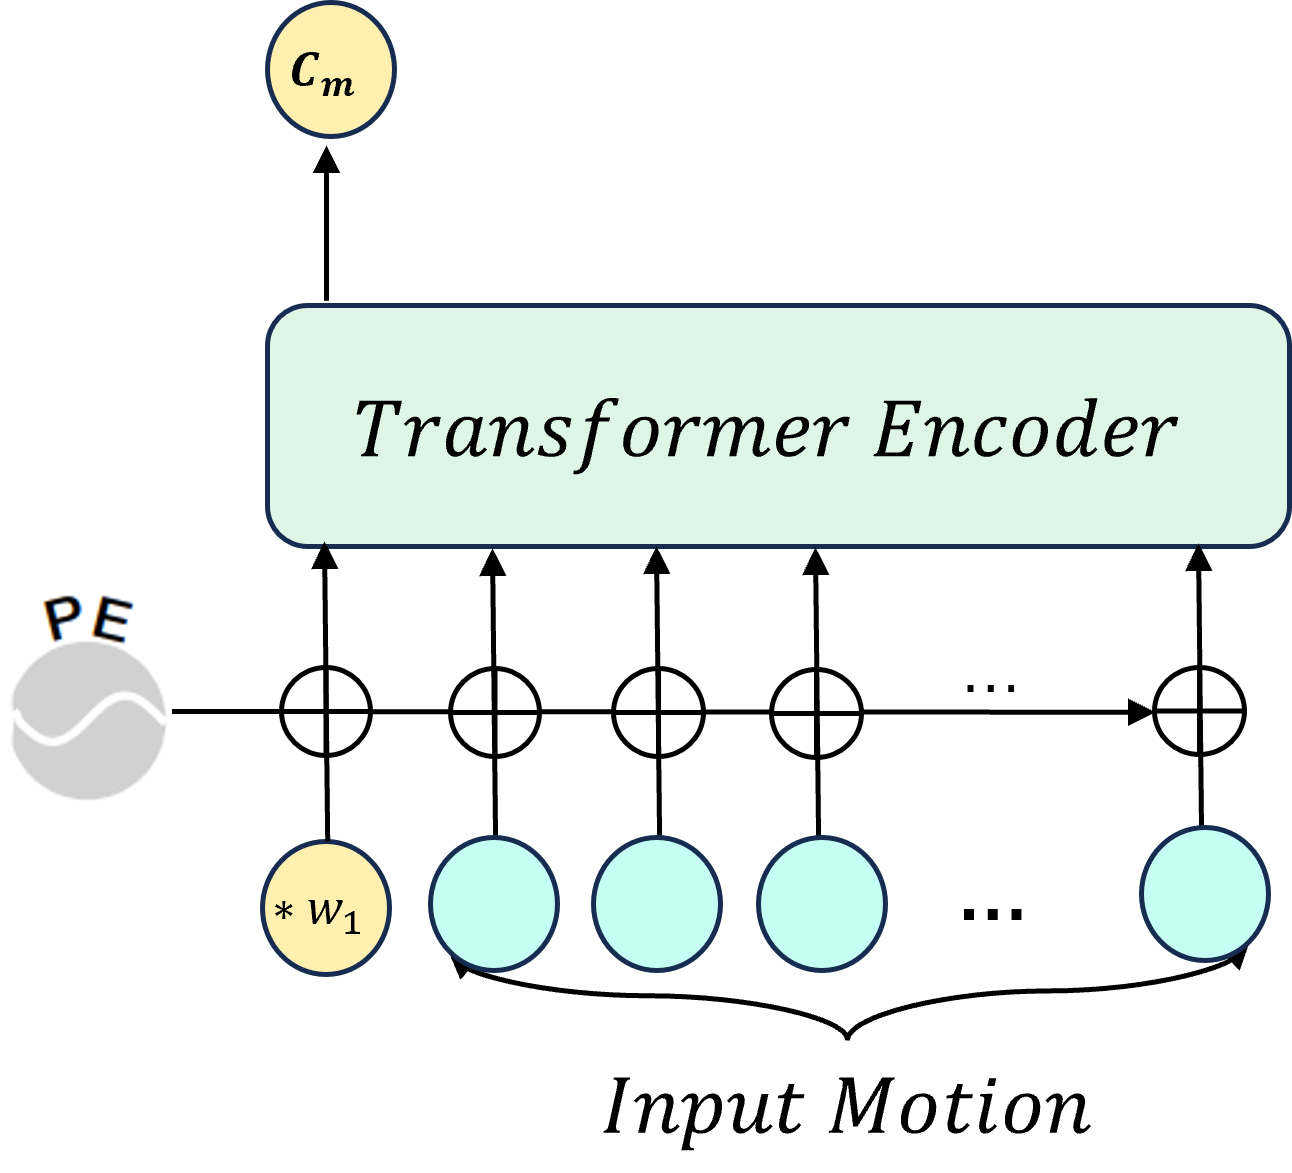
\includegraphics[width=0.45\textwidth]{figs/motion adapter.png}
    \caption{Lightweight transformer module for aligning motion data to the CLIP representation space.}
    \label{fig:motion_adapter}
\end{figure}

\paragraph{Architecture}
As sketched in Fig.~\ref{fig:whole_framework}, text conditions are encoded with a frozen CLIP text encoder,
\begin{equation}
c_t = \mathrm{CLIP}_t(I_t^{c}) \in \mathbb{R}^{1 \times 512},
\end{equation}
and motion conditions are projected into the same space via a lightweight transformer adapter \(W\) (Fig.~\ref{fig:motion_adapter}). The adapter consumes a sequence of poses and a learnable token and outputs a pooled representation
\begin{equation}
c_m = W(I_m^{c}) \in \mathbb{R}^{1 \times 512}.
\end{equation}
The adapter follows a standard encoder stack with self-attention and feed-forward blocks, with a small parameter budget to keep training stable and portable.

\paragraph{Training objective and data}
Given paired text–motion samples \((I_t^{c}, I_m^{c})\), the adapter is trained to align motion embeddings with their textual counterparts using cosine similarity:
\begin{equation}
\mathcal{L}_{\mathrm{align}} = 1 - \cos\big(\mathrm{CLIP}_t(I_t^{c}),\, W(I_m^{c})\big).
\end{equation}
Training uses HumanML3D pairs as the primary supervision, with the CLIP encoder frozen and only the motion adapter updated. Optimization employs Adam with a moderate learning rate and mini-batches sized to fully utilize a single high-end GPU. % 细节与数值可在实现节补充，与9月报告一致。

\paragraph{Interface to generation}
During this period the module was used as a representation component rather than a full control pathway. The unified embedding \(c\) can be exported to downstream generators as a conditioning vector alongside text, or used standalone for retrieval-style diagnostics. A text-only fallback is naturally available by omitting the motion branch.

\paragraph{Editing directions: offline analysis}
The aligned space admits linear directions of the form
\begin{equation}
c_{\mathrm{edit}} = c + \Delta c_{\mathrm{edit}},
\end{equation}
where \(\Delta c_{\mathrm{edit}}\) is computed from differences between target and source conditions in the shared space. In the first nine months this was investigated as an \emph{offline} feasibility analysis on embeddings and visualized motion proxies. A full editing/control pipeline integrated into the generator was not implemented in this period and is planned for subsequent stages. % 与前文“尚未实现控制”的表述一致。

\paragraph{Diagnostics and proxy metrics}
To probe whether the embedding geometry reflects desired semantics, I used retrieval precision and a proxy consistency score computed in the shared space. The latter compares distances between embeddings produced by text targets and embeddings produced by adapter-encoded motions after synthetic composition. These diagnostics are intended to complement distributional and retrieval metrics used later for generation. % 将具体数值移至实验节或附录，避免方法节堆砌表格。

\paragraph{Summary and lessons}
Learning a compact motion adapter aligned to a strong frozen text encoder yields a stable, fast-to-train conditional space that is easy to export to downstream models and analysis tools. The approach preserves a clean text-only path, and the embedding geometry supports linear composition analyses. The main limitation at this stage is the absence of an integrated control/editing pathway during inference; enabling such pathways and extending conditioning to short reference videos motivates the next stage of the project. % 为后续小节过渡。

\subsection{Video-Prior Enhanced Generation}
%==================== 3.2.1 ====================
% 说明：总览本阶段方法与训练/推理流程；强调控制尚未在前9个月实现，将在本阶段完成

% In the first nine months of this PhD, our work focused on establishing a multimodal conditional editing framework (MCRE) that unified text and motion signals in a shared space for controllable generation. While effective for text-driven editing, this framework lacked the ability to directly incorporate spatio-temporal priors from raw video inputs, which are abundant, semantically rich, and naturally aligned with human motion. This gap limited fine-grained control, temporal precision, and robustness under open-domain prompts. To address these limitations, we extend our baseline latent diffusion pipeline with video priors, aiming to combine the semantic expressiveness of textual inputs with the structural accuracy of video guidance. This leads to \textit{MotionDirector}, a multimodal framework that augments generation with video–text dual conditioning, distribution-aware alignment, and adaptive guidance.


% To augments the existing latent-diffusion baseline with video priors while keeping the editing hook in the shared condition space, We present MotionDirector, a novel multimodal framework for human motion synthesis that seamlessly integrates video and textual inputs to generate realistic, semantically coherent, and controllable motions. Fig. \ref{fig:motiondirector} shows an overview of the proposed framework. By leveraging a dual-conditioning paradigm, it combines video-driven spatio-temporal precision with text-guided semantic expressiveness. 
% Our framework comprises three key components: a conditional degradation-based guidance mechanism for efficient and controllable generation, DASH Loss for aligning generated motions with real-world distributions, and DUET, a unified multimodal encoder for cross-modal representation learning. In the following sections, we first describe the overall architecture and guidance mechanism, then formally derive the DASH Loss formulation, and finally provide a comprehensive description of DUET's design.

\textbf{Motivation and Relation to 9-Month Work.}
In the first nine months of this PhD, I developed the Multimodal Conditional Representation and Editing (MCRE) framework, which unified text and motion signals in a shared condition space for controllable editing. While MCRE was effective for text-driven editing, it did not directly exploit spatio-temporal priors from raw videos, which are abundant, semantically rich, and naturally aligned with human motion. Building on this foundation, I extend the latent-diffusion pipeline with video priors obtained from video foundation encoders such as VideoMAE~\cite{wang2023videomae}, thereby combining the semantic expressiveness of text with the structural accuracy of video guidance. This extension leads to MotionDirector, a multimodal framework that performs video–text dual conditioning, distribution-aware alignment, and adaptive guidance for high-fidelity and controllable motion synthesis.

\textbf{Backbones and my Extensions.}
The proposed framework relies on established components while extending them to the motion generation domain:
\begin{itemize}
    \item \textbf{Auto Guidance.} The method follows the idea introduced in Guiding a Diffusion Model with a Bad Version of Itself \cite{karras2024guiding} in Image generation. I adapt this principle to human motion generation by extrapolating between clean and degraded condition predictions during inference, thereby stabilizing guidance and improving temporal coherence.
    \item \textbf{Dual Conditioning Backbone.} For vision and text I employ pretrained encoders (VideoMAE for videos; CLIP for text) and fuse them into a unified condition through the DUET module. While standard fusion strategies are based on concatenation or cross-attention, our extension introduces adaptive and reliability-aware fusion (DMM) together with complementary frequency- and geometry-based branches.
    \item \textbf{Distribution-aware Alignment.} Beyond contrastive, triplet, or optimal transport objectives, I augment the standard MLD denoising loss with DASH Loss, which regularizes token-wise similarity and pairwise structural consistency between motion latents and video features. This formulation is specifically designed for motion–video alignment within diffusion.
\end{itemize}

% \textbf{Contributions.}
% The contributions of this work beyond the 9-month MCRE baseline are as follows:
% \begin{enumerate}
%     \item MotionDirector pipeline: a video–text dual-conditioning extension of a latent motion diffusion baseline that preserves the MCRE editing hook while incorporating video priors for spatio-temporal control.
%     \item Auto Guidance for motion: a domain-specific adaptation of clean–degraded extrapolation to replace unconditional CFG in motion generation, improving balance and temporal stability without additional training.
%     \item Feature-space conditional perturbation: a training-free guidance tuning strategy that perturbs fused condition embeddings with dropout or Gaussian noise to simulate weak conditions and enable discrete search over guidance weights with reduced instability.
%     \item DASH Loss: a distribution-aware alignment loss combining token-level semantic margins and pairwise structural consistency between denoiser hidden states and VideoMAE features.
%     \item DUET module: a multimodal fusion block with Dynamic Mask Mechanism for reliability-aware feature selection, an FFT branch for global periodicity, and a local convolutional branch for spatial refinement, combined with residual connections for stability.
% \end{enumerate}


\subsubsection{Auto-Guided Dual Conditioning}

MotionDirector employs a dual-conditioning paradigm, simultaneously leveraging both video and textual inputs to guide motion generation. Video inputs provide explicit spatio-temporal trajectory control, while textual inputs deliver essential semantic guidance.


\paragraph{Vision and Text Conditioning}
To provide multimodal guidance, I employ two pretrained encoders: a VideoMAE-based Vision Transformer $\mathcal{E}_{\text{Vim}}$ \cite{wang2023videomae} for video input and a CLIP Text Encoder $\mathcal{E}_{\text{CLIP}}$ for textual prompts. Given an input video $I \in \mathbb{R}^{C \times L \times H \times W}$ and a text prompt $\mathbf{t}$, I obtain the visual feature sequence $\mathbf{V} = \mathcal{E}_{\text{Vim}}(I)$ and the text embedding $\mathbf{T} = \mathcal{E}_{\text{CLIP}}(\mathbf{t})$, which are jointly used for conditioning downstream modules.

\paragraph{Multimodal Fusion with Auto Guidance}

Traditionally, CFG applies separate weights to each modality to control their influence during inference, e.g.,

\begin{equation}
\nabla \log p(\mathbf{x}_t \mid \mathbf{V}, \mathbf{T}) \approx \omega_{\text{v}} \nabla \log p(\mathbf{x}_t \mid \mathbf{V}) \\ 
+ \omega_{\text{t}} \nabla \log p(\mathbf{x}_t \mid \mathbf{T}),
\end{equation}

where $\omega_{\text{v}}$ and $\omega_{\text{t}}$ are manually tuned weights for the vision and text conditions, respectively.

To enable joint modeling of modalities, I employ a fusion module $\mathcal{F}_{\text{DUET}}$ during training to encode visual and textual inputs into a unified representation:
\begin{equation} \label{eqn:F}
\mathbf{H} = \mathcal{H}_{\text{DUET}}(\mathbf{V}, \mathbf{T}).
\end{equation}
This design treats $\mathbf{V}$ and $\mathbf{T}$ as correlated signals governed by a joint distribution \( p(\mathbf{x}_t \mid \mathbf{V}, \mathbf{T}) \), allowing the model to learn their mutual dependencies and internal balancing.

At inference time, the model will apply a unified CFG weight over the fused representation $\mathbf{H}$:
\begin{equation}
% \small
\nabla \log p(\mathbf{x}_t \mid \mathbf{H}) \approx (1 \!+\! \omega) \nabla \log p(\mathbf{x}_t \mid \mathbf{H}) \!-\! \omega \nabla \log p(\mathbf{x}_t),
\end{equation}
However, such CFG-based strategies suffer from sensitivity to manually tuned weights, often leading to suboptimal balance and unstable gen. Moreover, they lack an internal correction mechanism to compensate for degraded outputs.


To address these limitations, I introduce Auto Guidance, which refines clean predictions \(\mathcal{M}_1\) by incorporating degraded predictions during inference. Specifically, I utilize degraded models, \(\mathcal{M}_2\), each configured with reduced conditioning strength. During training, the model is trained with full conditioning. During inference, the final denoising result is computed as:
\begin{equation}
M_{\text{auto}}(\mathbf{x}_t; \sigma, \mathbf{V}, \mathbf{T}) = M_1(\mathbf{x}_t; \sigma, \mathbf{V}, \mathbf{T}) \\
+ \omega \left( M_1(\mathbf{x}_t; \sigma, \mathbf{V}, \mathbf{T}) - M_2(\mathbf{x}_t; \sigma, \mathbf{V}, \mathbf{T}) \right).
% \tag{4}
\end{equation}
where \( \omega \) is a fixed extrapolation factor, the symbol $\sigma$ denotes the diffusion \emph{noise level} (i.e., the standard deviation of the Gaussian noise at the current timestep). Unlike conventional CFG, this approach does not rely on an unconditional model and avoids manual weight selection. We treat the clean condition as a semantic anchor, enabling the model to interpret the deviation  as a meaningful correction direction. 




\begin{figure}[t]
    \centering
    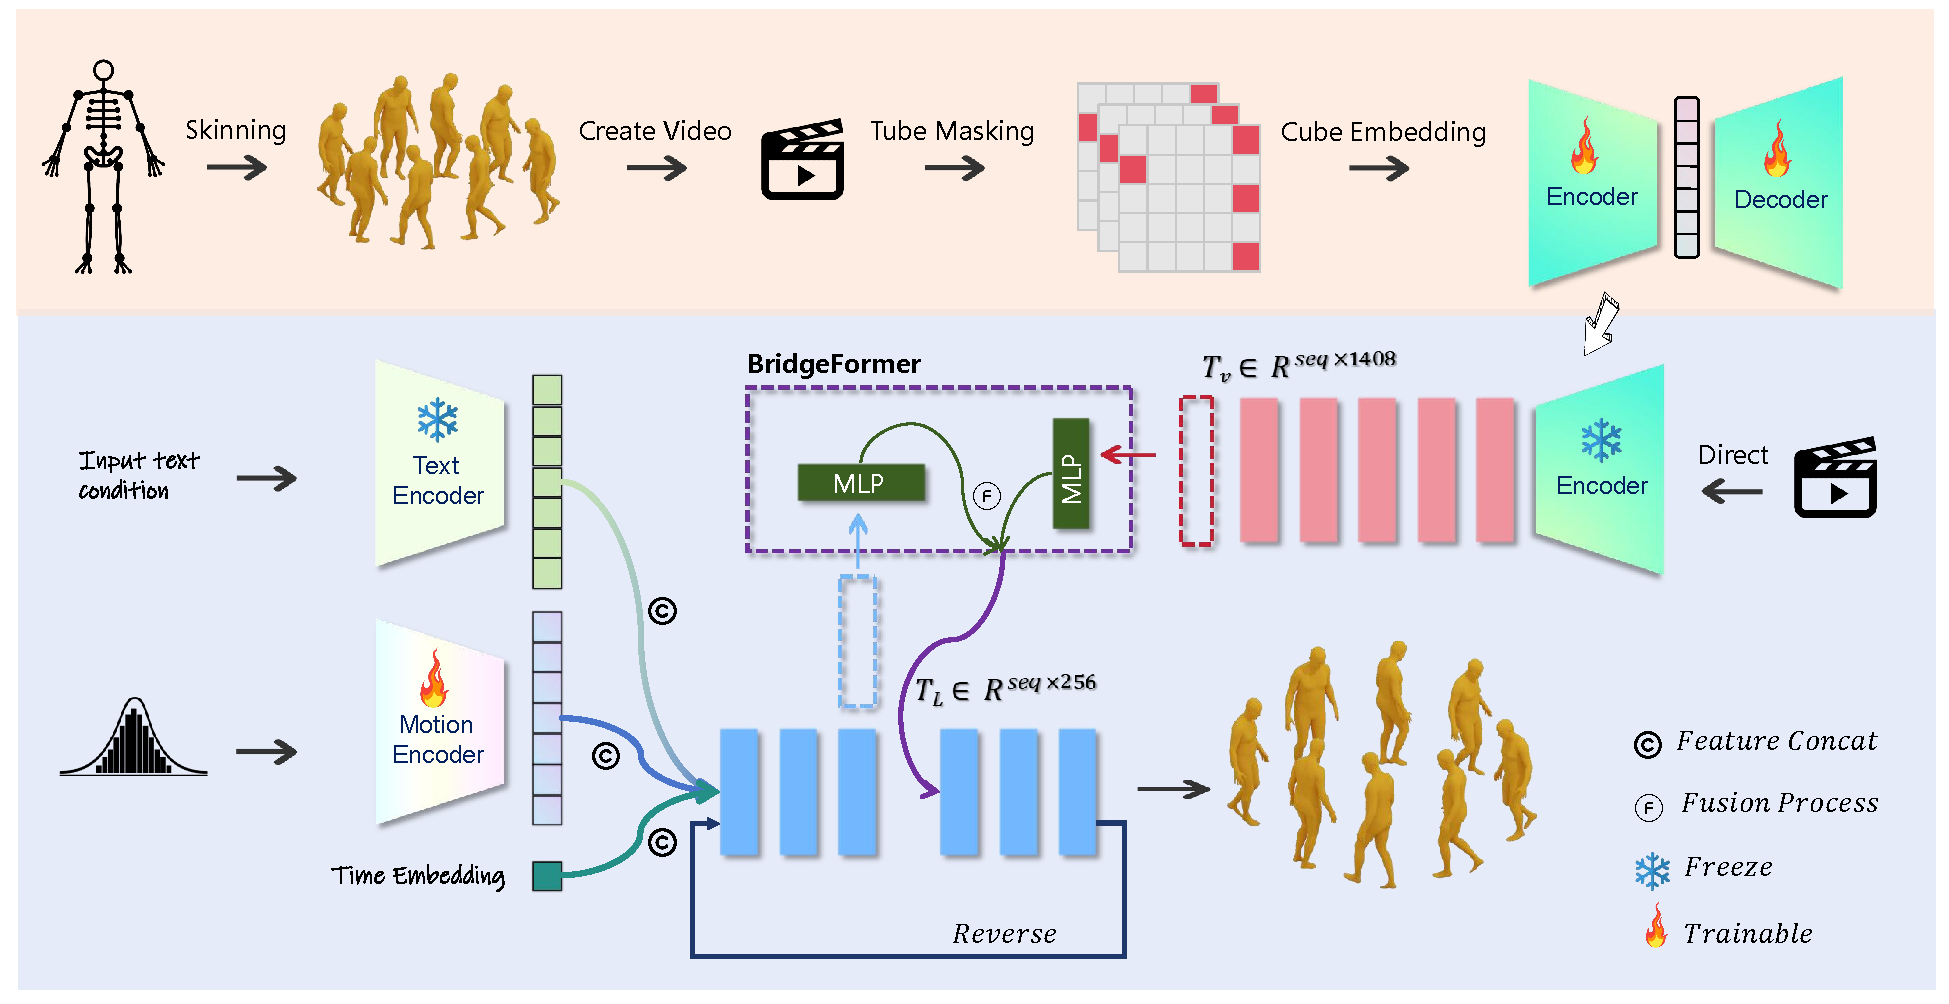
\includegraphics[width=\textwidth]{fig_motion_Director/MotionDir_new.pdf}
    \caption{MotionDirector framework overview. It primarily consists of three key steps: 1) fine-tuning video motion dataset based on a pre-trained model and freezing the weights to focus on inference (orange background); 2) proposing a dual-stream control mechanism combined with auto-guidance mechanism to integrate video and text inputs, effectively guiding motion generation (blue background); and 3) utilizing the DUET module (purple dashed box) combined with DASH Loss to align and fuse multimodal information, enhancing overall information processing capabilities.}
    \label{fig:motiondirector}
\end{figure}

\subsubsection{Auto Guidance via Feature-Space Conditional Perturbation}

To enable adaptive dual-conditioning in multimodal diffusion without retraining or manual tuning, I propose a lightweight guidance optimization strategy based on feature-space conditional perturbation. Unlike prior works~\cite{karras2024guiding} that simulate weak conditions via input masking or model degradation, I directly perturb the fused representation $\mathbf{H}$ in feature space. This approach preserves the pretrained model weights and enables efficient guidance optimization without architecture changes, while accounting for the inherent structural differences across modalities: text embeddings are dense and semantically fragile, whereas video features exhibit high spatial-temporal redundancy and are more tolerant to perturbations.

\paragraph{Feature-Space Perturbation}
Given the fused embedding $\mathbf{H}$ (\textit{cf.} Eq.~\eqref{eqn:F}), I simulate degraded conditions using two forms of perturbation:

\begin{itemize}
    \item \textbf{Dropout Perturbation ($\mathcal{D}$):} Randomly zeros a proportion $p$ of feature dimensions:
    \begin{equation}
        \tilde{\mathbf{H}}^{(\mathcal{D})} = \text{Dropout}(\mathbf{H}; \mathcal{D}).
    \end{equation}

    \item \textbf{Gaussian Noise Perturbation ($\sigma$):} Adds isotropic Gaussian noise:
    \begin{equation}
        \tilde{\mathbf{H}}^{(\sigma)} = \mathbf{H} + \epsilon, \quad \epsilon \sim \mathcal{N}(0, \sigma^2).
    \end{equation}
\end{itemize}

These operations simulate weaker or noisier conditions in latent space without altering the model architecture or requiring retraining.

\paragraph{Auto Guidance with Perturbed Features}
Instead of relying on clean and null conditions as in classifier-free guidance, I guide the generation using a clean embedding and its degraded counterpart with controlled noise, denoted as $\tilde{\mathbf{H}}^{\text{strong}}$ and $\tilde{\mathbf{H}}^{\text{weak}}$. The final output is computed as:
\begin{equation}
\hat{\mathbf{x}}_t = (1 + \omega) \cdot \hat{\mathbf{x}}_t^{\text{strong}} - \omega \cdot \hat{\mathbf{x}}_t^{\text{weak}},
\end{equation}
where $\hat{\mathbf{x}}_t^{\text{strong}}$ and $\hat{\mathbf{x}}_t^{\text{weak}}$ are predictions conditioned on the corresponding clean and degraded features.

This formulation preserves the consistency of the latent space while enabling gradient-free guidance tuning. It eliminates the need for an unconditional path, reduces sampling instability, and avoids distortions caused by overconfident guidance weights.

I perform a discrete search over $\omega$ using fixed degradation levels and select the optimal $\omega^*$ based on val metrics including motion realism, semantic fidelity, and FID.

\subsubsection{Multimodal Denoising Objective}

MotionDirector adopt a denoising objective inspired by the MLD paradigm \cite{chen2023executing}, which formulates motion generation as a conditional diffusion process guided by multimodal contexts. Given a clean motion sequence $\mathbf{x}_0$ and its noisy version $\mathbf{x}_t$ at diffusion timestep $t$, the model learns to obtain the predicted latent $\hat{\mathbf{z}}_t$ using multimodal condition $\mathbf{c} = (\mathbf{V}, \mathbf{T})$ (which contains text and video embeddings extracted by frozen encoders), i.e.,
$
\hat{\mathbf{z}}_t = \mathcal{D}_\theta(\mathbf{x}_t, t, \mathbf{c}),
$
where $\mathcal{D}_\theta$ is the denoising network (a Transformer-based decoder).
%
The training objective minimizes the mean squared error between the predicted latent $\hat{\mathbf{z}}_t$ and the diffusion target  $\mathbf{z}_{\text{target},t}$, i.e.,
\begin{equation}
\mathcal{L}_{\text{MLD}} = \mathbb{E}_{\mathbf{x}_0, t, \boldsymbol{\epsilon}} \left[ \left\| \hat{\mathbf{z}}_t - \mathbf{z}_{\text{target},t} \right\|^2 \right].
\end{equation}

This serves as the primary supervision signal for motion generation, with additional guidance losses applied on latent representations as detailed below.

\subsubsection{Distribution-aware Training with DASH Loss}

To bridge the distributional gap between generated latent motions and real video-conditioned embeddings, I propose the \textbf{DASH} \textbf{Loss}. Established objectives such as \textit{Contrastive Loss}~\cite{radford2021learning}, \textit{Triplet Loss}~\cite{schroff2015facenet}, and \textit{Optimal Transport Loss}~\cite{peyre2019computational}, which mainly emphasize global matching or rigid structural mappings, often overlook fine-grained token-level misalignments and lack explicit structural regularization. Consequently, they may fail to capture nuanced correspondences and lead to unstable training dynamics. Our DASH loss regularizes the learned motion representations by enforcing both \emph{token-level similarity} and \emph{structural consistency} with the video-conditioned features.
%
Specifically, I extract:
\begin{itemize}
    \item Motion feature tokens \(\hat{\mathbf{z}}_{t,\text{d}}\), denoting the hidden representation extracted from the \textit{d}-th layer of our denoising transformer network at diffusion timestep \(t\), which captures rich intermediate-level structural cues. The network input is composed of motion latents, text, and temporal embeddings.
    \item Video reference features \(\mathbf{V}\) from the VideoMAE encoder (\textit{cf.} Eq.~(\ref{eqn:F})), which encode spatial-temporal dynamics from video inputs.
\end{itemize}

Here, each sample point \(i = 1, \dots, N\) corresponds to a matched pair \((\hat{z}_{t,\text{d},i}, v_i)\), representing aligned motion and video tokens within the same temporal segment.

\paragraph{Token-wise Margin Loss}
I first align individual latent tokens to their video-conditioned counterparts using a margin-based cosine similarity loss, i.e.,
% \begin{equation}
% \mathcal{L}_{\text{token}} = \frac{1}{N} \sum_{i=1}^{N} \text{ReLU} \left( 1 - m_{\text{cos}} - \cos(\hat{z}_i, f_i) \right),
% \end{equation}
\begin{equation}
\mathcal{L}_{\text{token}} = \frac{1}{N} \sum_{i=1}^{N} \text{ReLU} \left( 1 - m_{\text{cos}} - \cos(\hat{z}_{t,\text{d},i}, v_i) \right),
\end{equation}
where $\cos(\cdot,\cdot)$ denotes the cosine similarity, and $m_{\text{cos}}$ is a predefined margin. This loss penalizes only those token pairs whose similarity falls below the margin, promoting semantic alignment without over-constraining well-matched pairs.

% \subsubsection{Pairwise Structure Alignment.}
\paragraph{Pairwise Structure Alignment}
To preserve the global structure of the feature space, I introduce a structural consistency loss that aligns the pairwise similarity between token pairs within each modality, i.e.,
\begin{equation}
\mathcal{L}_{\text{pair}} = \frac{1}{N^2}\sum_{i,j=1}^{N} \text{ReLU} \big( | \cos(\hat{z}_{t,\text{d},i}, \hat{z}_{t,\text{d},j}) - \cos(v_i, v_j) | - m_{\text{pair}} \big),
\end{equation}
% \begin{equation}
% \mathcal{L}_{\text{pair}} = \frac{1}{N^2} \sum_{i,j=1}^{N} \text{ReLU} \left( \left| \cos(\hat{z}_i, \hat{z}_j) - \cos(f_i, f_j) \right| - m_{\text{pair}} \right),
% \end{equation}
where $m_{\text{pair}}$ is a margin threshold. This formulation encourages the relative structure of the motion latent space to mirror that of the video-conditioned embedding space.


% \subsubsection{Overall Loss Formulation.}
\paragraph{Overall Loss Formulation}
The full DASH loss is given by a weighted sum of the two objectives, i.e.,
\begin{equation}
\mathcal{L}_{\text{DASH}} = \mathcal{L}_{\text{token}} + \mathcal{L}_{\text{pair}}.
\end{equation}

% where $\lambda_{\text{token}}$ and $\lambda_{\text{pair}}$ are hyperparameters controlling the balance between local and global alignment.

Finally, the total training loss combines the latent diffusion reconstruction objective $\mathcal{L}_{\text{MLD}}$ with our proposed alignment regularizer, i.e.,
\begin{equation}
\mathcal{L} = \mathcal{L}_{\text{MLD}} + \lambda_{\text{DASH}} \mathcal{L}_{\text{DASH}}.
\end{equation}
%
This distribution-aware training scheme enhances both semantic fidelity and structural coherence of the generated motions, enabling more expressive and controllable motion synthesis across modalities.


\begin{figure}[t]
    \centering  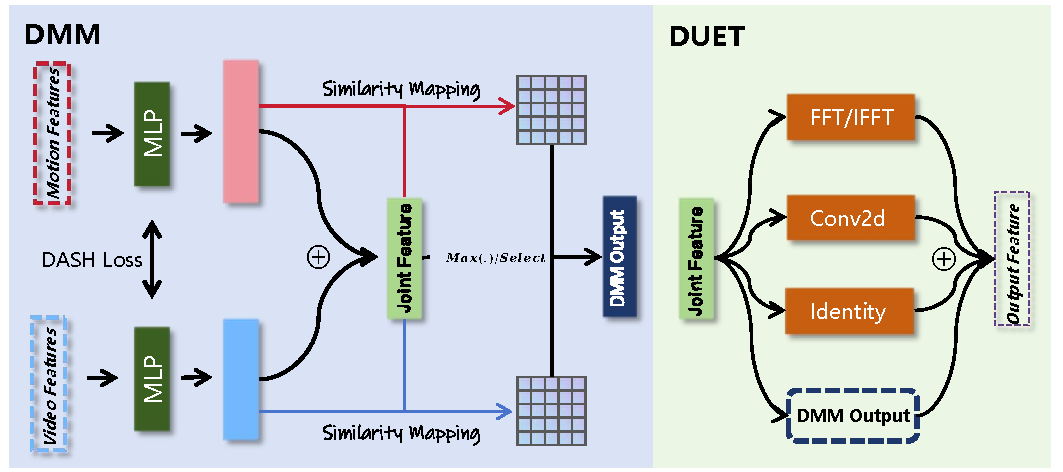
\includegraphics[width=1.05\linewidth]{fig_motion_Director/submodule.pdf}
    \caption{Illustration of the overall DUET multimodal fusion architecture. DUET consists of DMM for adaptive alignment, an FFT-based branch for global frequency encoding, residual connections to preserve fine details, and a local convolutional for spatial refinement.}
    % \xc{The label is the same as the label used in Figure 1, which is not right. Also, this figure is not introduced in the main text?}}
    \label{fig:DUET}
\end{figure}

\subsubsection{DUET: Dual-stream Unified Encoding and Transformation}
Common fusion strategies such as element-wise addition, concatenation, and cross-modal attention are widely adopted in multi-modal learning due to their simplicity and generality. However, these methods typically treat all modalities uniformly, ignoring potential variations in quality or informativeness across inputs. When one modality is noisy or unreliable, such naive aggregation can introduce interference and degrade the overall performance.

The design of DUET was driven by a series of empirical observations made throughout our research. 
In earlier work on multimodal conditional generation task, we found that simple fusion strategies (e.g., element-wise addition, concatenation, or cross-attention) often struggled to maintain semantic consistency when one modality was degraded or noisy. 
This problem became more evident when extending to video–motion fusion in MotionDirector, where a significant proportion of automatically rendered videos exhibited artifacts, and annotation errors (see Appendix~\ref{Automated Video Data Cleaning}). 
These inconsistencies motivated the introduction of a mechanism that could adaptively suppress unreliable modality features while preserving informative ones.

To further enhance representational richness, DUET integrates four complementary branches: the FFT branch captures global periodicity and temporal regularities; the convolutional branch focuses on geometric representations and local spatial refinement; the Dynamic Mask Mechanism (DMM) adaptively selects semantically aligned and reliable features across modalities; and the residual connection helps preserve original information and stabilize the fusion process. This synergy ensures that both global structure and local details are preserved, while noisy or inconsistent inputs are effectively suppressed, as illustrated in Fig.~\ref{fig:DUET}.

By integrating all four components, DUET provides both robustness to noisy conditions and enriched representational capacity, as confirmed in the ablation study (Table~\ref{tab:fusion_strategies}), where the full module consistently outperforms its reduced variants.


\paragraph{Fast Fourier Transform}
Human motions inherently exhibit periodic or quasi-periodic structures, particularly in locomotion and other repetitive behaviors such as walking, running, and marching. These temporal patterns are especially prominent in video inputs, which naturally encode rich spatio-temporal cues and sequential dynamics. Such patterns are compactly expressed in the frequency domain, where they can be effectively disentangled from noise.

 The input fused feature say $R \in \mathbb{R}^{B \times T \times D}$ is first transformed into the frequency domain via FFT, i.e., $\mathcal{F}(R)$. Rewriting
\begin{equation}
\mathcal{F}(R) = \hat{R}_{\rm real} + j \hat{R}_{\rm im},
\end{equation}

where $\hat{R}_{\rm real}$ and $\hat{R}_{\rm im} \in \mathbb{R}^{B \times T \times D}$ are the real and imaginary components, respectively. These are concatenated and modulated using a depthwise $1 \times 1$ convolution for frequency-wise filtering, i.e.,
\begin{equation}
    [\hat{R}_{\rm real}', \hat{R}_{\rm im}'] = \text{Conv1x1}([\hat{R}_{\rm real}, \hat{R}_{\rm im}]).
\end{equation}
The enhanced representation is reconstructed via inverse FFT, i.e., $ \small F = \mathcal{F}^{-1}(\hat{R}_{\rm real}' + j \hat{R}_{\rm im}'), $ where $F \in \mathbb{R}^{B \times T \times D}$ denotes the frequency-aware output.


\paragraph{Dynamic Mask Mechanism}
% FFT 关注的运动的频率，Conv 几何表征，dmm特征之间的信息
During the visualization of video inputs, I observed that some samples suffer from noticeable quality issues (see \ref{Automated Video Data Cleaning}). As the primary source of guidance for motion generation, these low-quality videos can introduce noise and undermine the overall fusion performance. To address the inconsistency in modality quality, I proposed Dynamic Mask Mechanism(DMM) which enables the model to automatically identify and retain modality-specific features that are more semantically consistent and informative. This selective fusion strategy helps improve the coherence and robustness of motion generation.

Given two input modality features, we aim to dynamically select more reliable information based on their semantic alignment with a shared latent representation. To initiate cross-modal interaction, we compute an initial fused representation via element-wise addition, i.e.,
\begin{equation}
    \mathbf{R} = \hat{\mathbf{z}}_{t,\text{d}} + \mathbf{V},
\end{equation}
where \(\mathbf{R}\) serves as the preliminary modality-integrated representation. This fused vector encodes shared spatial and semantic information across both modalities, and is subsequently refined by the DMM to adaptively emphasize more reliable features based on their alignment with a latent guidance signal.

To enhance semantic consistency across modalities, the DMM inter-modal similarity by projecting the fused features into a compact latent space using a feedforward network, followed by reconstruction via a lightweight decoder. This process spatially aligns features from both conditional branches within a shared target space, enabling precise and coherent output generation. We use the Euclidean distance between the two as a measure of similarity, i.e.,
\begin{equation}
\text{Dist}_{\hat{\mathbf{z}}_{t,\text{d}}} = \left\| \mathbf{R} - \hat{\mathbf{z}}_{t,\text{d}} \right\|_2,
\text{Dist}_{\mathbf{V}} = \left\| \mathbf{R} - \mathbf{V} \right\|_2.
\end{equation}

The selection of features is determined based on the relative values of the similarity map. Specifically, the features that are more similar to the shared representation are retained, while those that are less similar are discarded. The selection rule is defined as
\begin{equation}
    \text{Mask} =
\begin{cases}
0, & \text{if } \text{Dist}_{\hat{\mathbf{z}}_{t,\text{d}}} \geq \text{Dist}_{\mathbf{V}}, \\
1, & \text{if } \text{Dist}_{\hat{\mathbf{z}}_{t,\text{d}}} < \text{Dist}_{\mathbf{V}}.
\end{cases}
\end{equation}

The FFT and conv branches are implemented in parallel rather than sequentially after DMM, as DMM may suppress informative regions and limit subsequent receptive fields.




\newpage

%==================== 3.3 ====================
\subsection{Hierarchical One-Pass Autoregressive Generation (Infinite-Length)}
% In the 9-month report, one of the identified limitations was the restricted temporal horizon of existing text-to-motion models, which are typically confined to short clips (around 10–12 seconds). This constraint hinders applications such as virtual avatars, gaming, or long-form animation, where continuous and coherent motion over extended durations is critical. As outlined in the future work plan, the second year of this PhD focuses on developing a framework capable of \emph{infinite-length generation}. To address this, we developed \textbf{MOGO}, a purely autoregressive framework that leverages hierarchical residual quantization and causal decoding to produce semantically consistent motions at arbitrary lengths, while also remaining compatible with real-time continuation and prompt switching.

% Our proposed framework, MOGO, as showned in Fig.~\ref{fig:architechure1}, consists of four key components designed for efficient and expressive text-to-motion generation. First, MoSA-VQ discretizes motion sequences into multi-level latent tokens using hierarchical residual quantization with adaptive scaling. Second, RQHC-Transformer autoregressively decodes the quantized representations with a stack of level-aligned transformer blocks. Third, MOGO supports infinite-length generation via seamless autoregressive extension. Lastly, we introduce TCA to enhance generalization to real-world prompts. We elaborate on each component in the following subsections.

In the 9-month report, one of the identified limitations was the restricted temporal horizon of existing text-to-motion models, which are typically confined to short clips (around 10--12 seconds). This constraint hinders applications such as virtual avatars, gaming, or long-form animation, where continuous and coherent motion over extended durations is critical. As planned for the second year, this PhD focuses on developing a framework capable of infinite-length generation. This subsection reports a joint academia–industry effort conducted with VLC lab colleague \textbf{Pengcheng Fang} and our industry collaborator \textbf{Dongjie Fu}. My primary responsibility was the design and implementation of the MoSA-VQ inference pathway for infinite-length continuation. In addition, together with Pengcheng and Dongjie, I co-led the implementation of the RQHC-Transformer and the TCA inference enhancement.

We developed MOGO, a purely autoregressive framework that leverages hierarchical residual quantization and causal decoding to produce semantically consistent motions at arbitrary lengths, while also remaining compatible with real-time continuation and prompt switching.

Our proposed framework, MOGO, as shown in Fig.~\ref{fig:architechure1}, consists of four key components designed for efficient and expressive text-to-motion generation. First, MoSA-VQ discretizes motion sequences into multi-level latent tokens using hierarchical residual quantization with adaptive scaling. Second, RQHC-Transformer autoregressively decodes the quantized representations with a stack of level-aligned transformer blocks. Third, MOGO supports infinite-length generation via seamless autoregressive extension. Lastly, MOGO introduce TCA to enhance generalization to real-world prompts. We elaborate on each component in the following subsections.



\begin{figure*}[!t] % 使用 figure 环境来处理图片
    \centering
    % 按照屏幕宽度自适应，高度保持比例填充
    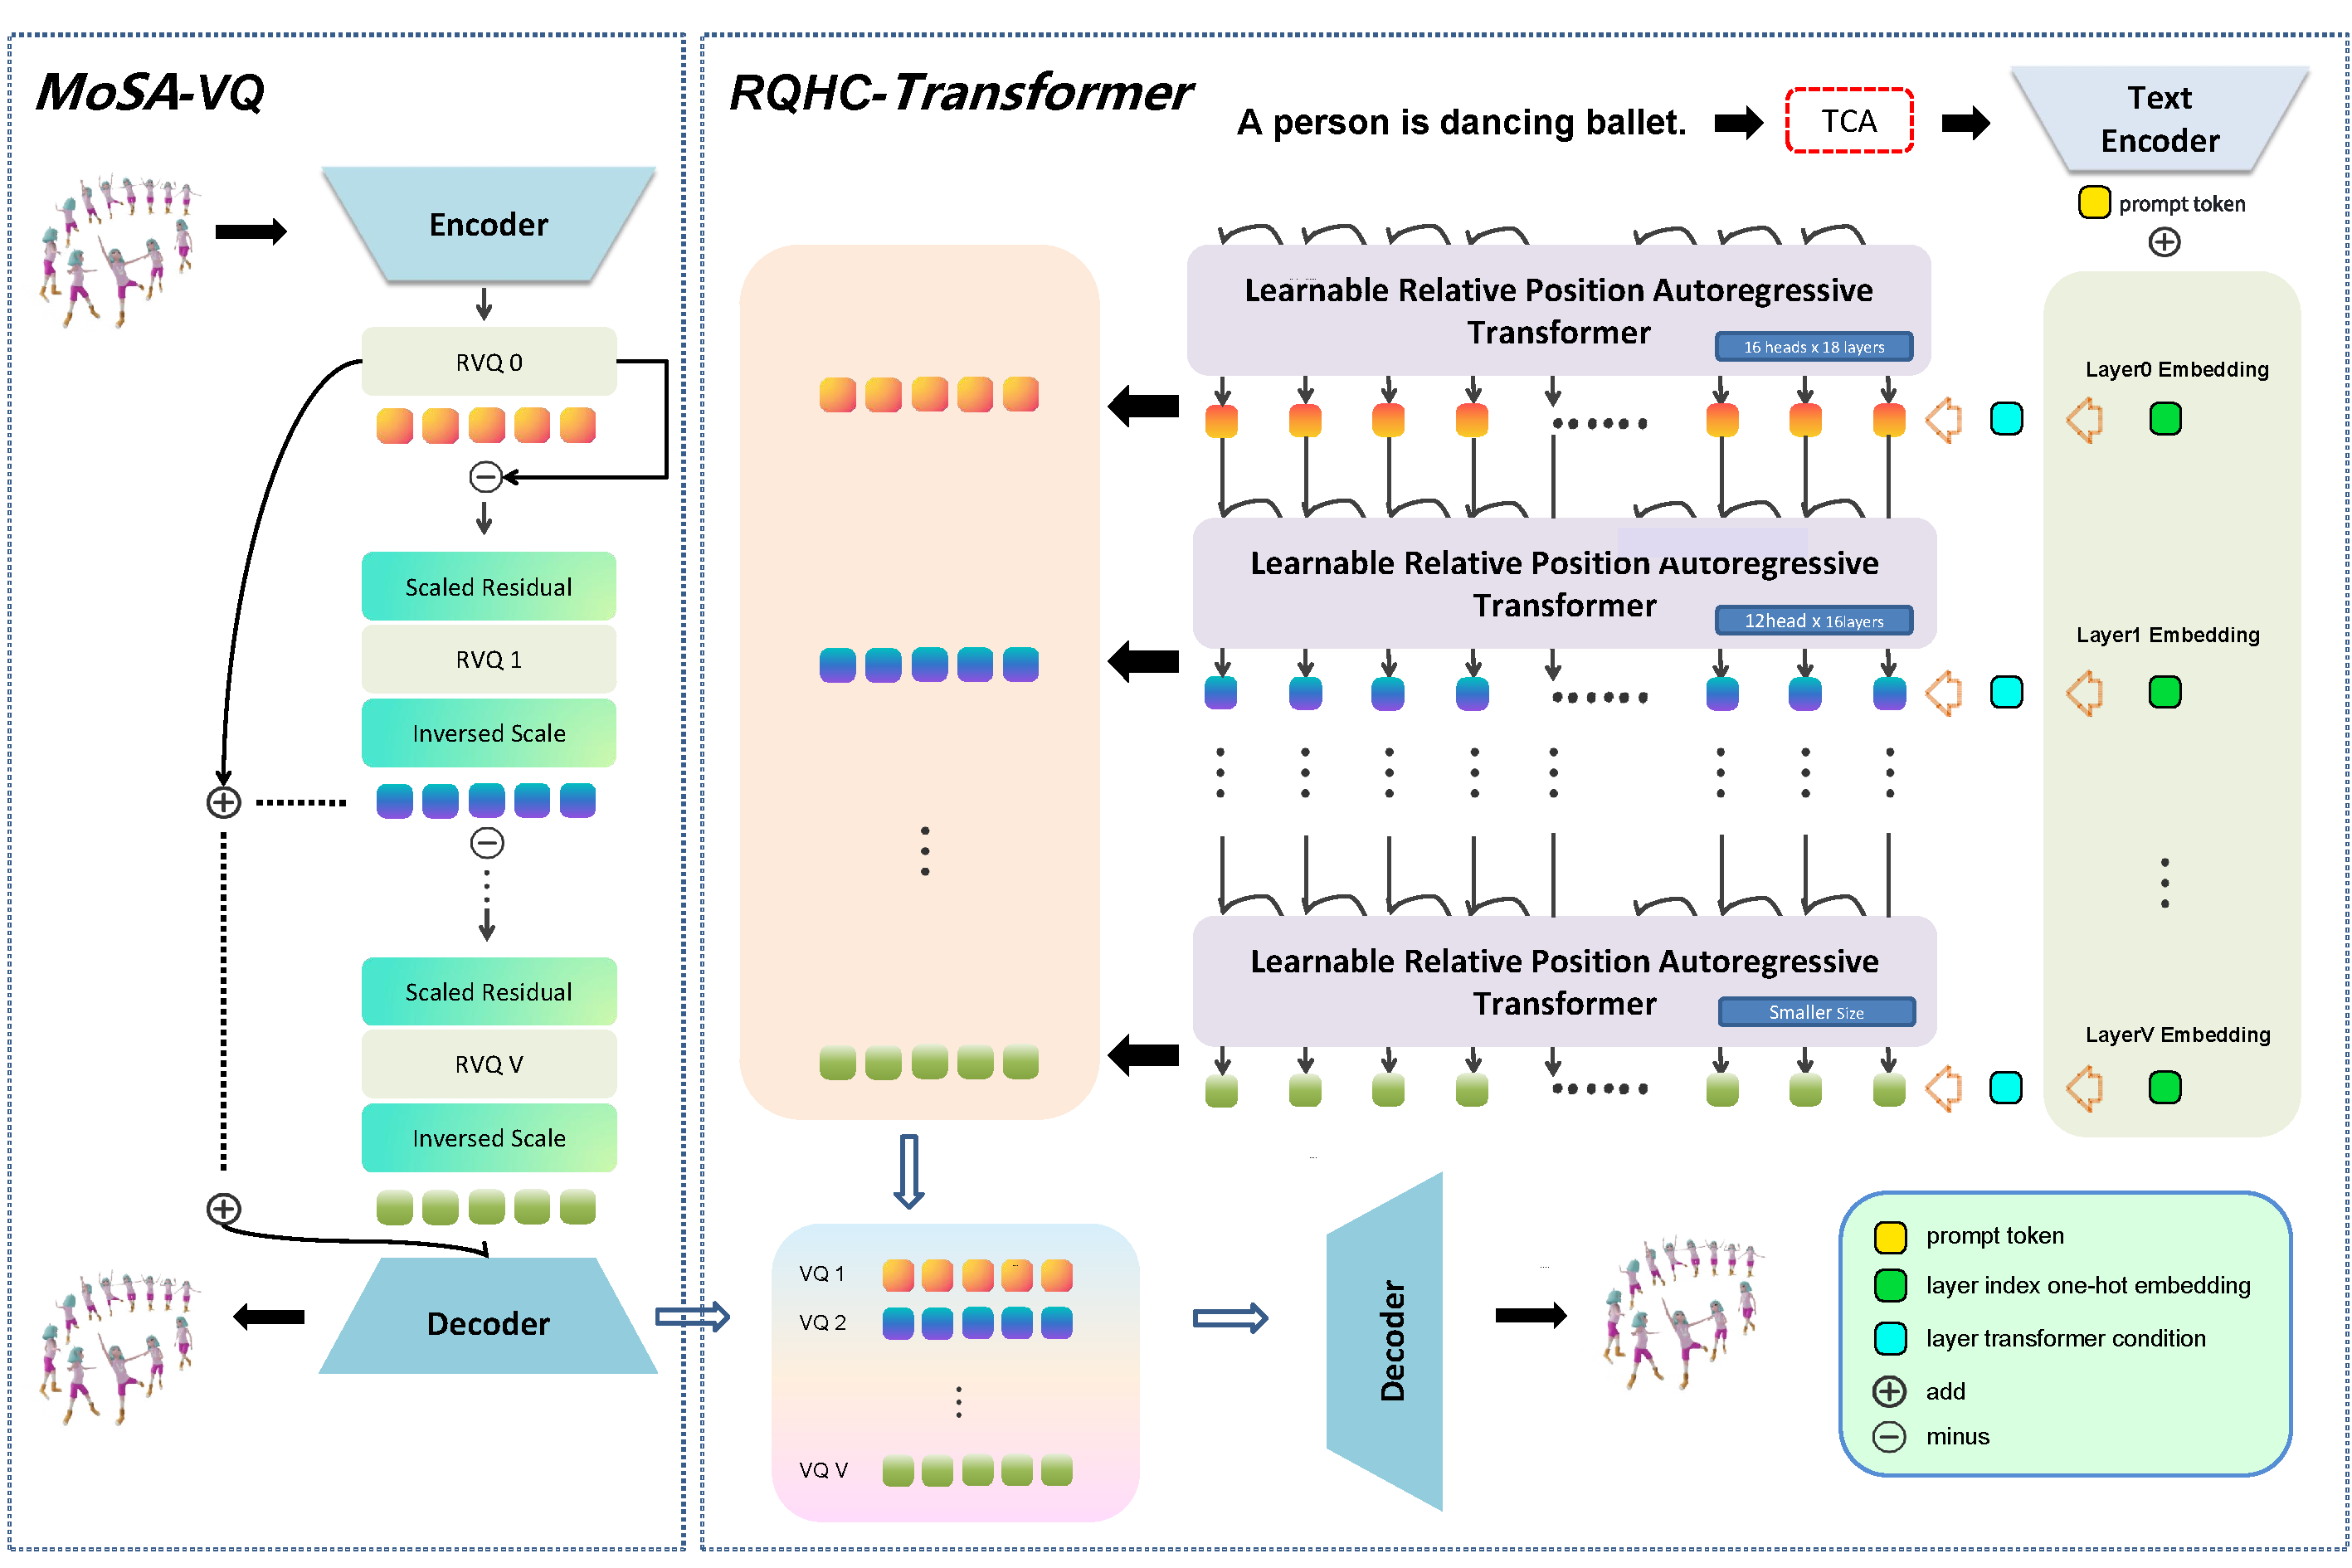
\includegraphics[width=0.98\textwidth]{fig_mogo/Mogo_main.pdf}
    \caption{Overview of the proposed MOGO framework. \textit{Left}: We first encode the motion sequence using a hierarchical MoSA-VQ module with learnable feature scaling, indexing a multi-level codebook. \textit{Right}: Then, tokens are autoregressively generated by a RQHC-Transformer with relative positional attention. Finally, the predicted token sequence is quantized and decoded into a full 3D human motion sequence.}

    \label{fig:architechure1} % 添加图片标签
\end{figure*}

\subsubsection{Hierarchical Tokenization}
\label{sec:rvqvae}
To transform continuous human motion into discrete representations suitable for autoregressive generation, I build upon residual vector quantized variational autoencoders (RVQ-VAEs) and propose MoSA-VQ. While standard RVQ-based approaches~\cite{guo2024momask, zhong2023attt2m} hierarchically encode motion features through fixed-stage quantization, they often rely on manually tuned feature ranges and static scaling behavior, which limit their adaptability and quantization efficiency—especially in the presence of diverse and complex motions.

\paragraph{Adaptive Hierarchical Quantization}
To address these limitations, I introduce a learnable feature scaling mechanism into each quantization level. Specifically, each level is equipped with its own learnable scale and bias parameters, which dynamically adjust the amplitude and offset of the input residual features before quantization. This adaptive design allows each level to allocate representational capacity where needed, resulting in more effective codebook usage and higher reconstruction accuracy without the need for handcrafted calibration.


At each hierarchical quantization level \( l \in \{0, 1, \ldots, L\} \), the residual vector is first transformed using a learnable affine mapping, which denoted as:
\begin{equation}
\mathbf{q}^l = \mathcal{Q}(\mathbf{W}^l \mathbf{r}^l + \mathbf{b}^l), \quad 
\boldsymbol{\phi}^l = (\mathbf{W}^l)^{-1} (\mathbf{q}^l - \mathbf{b}^l),
\end{equation}
where \( \mathbf{W}^l \in \mathbb{R}^{d \times d} \) is a diagonal scaling matrix, \( \mathbf{b}^l \in \mathbb{R}^d \) is a learnable bias vector, \( \mathcal{Q}(\cdot) \) denotes nearest-neighbor quantization via a codebook, and \( \boldsymbol{\phi}^l \) represents the decoded contribution at level \( l \).


This hierarchical quantization scheme enables progressive residual refinement. Unlike conventional residual vector quantization (RVQ) frameworks that apply uniform scaling across all levels, this design introduces level-specific adaptive modulation through learnable parameters \( \mathbf{W}^l \) and \( \mathbf{b}^l \). This flexibility allows coarse levels to capture global structure, while deeper layers focus on subtle motion or spatial details. The inverse affine transformation ensures consistent feature recovery, and stride-1 convolutions in both encoder and decoder maintain temporal continuity without aliasing artifacts. We have
\begin{equation}
\mathbf{r}^{l+1} = \mathbf{r}^l - \boldsymbol{\phi}^l, \quad
\hat{\mathbf{z}} = \sum_{l=0}^{L} \boldsymbol{\phi}^l.
\end{equation}


\paragraph{Training Objective}
The full training objective combines four terms: motion reconstruction, codebook commitment, lightweight modulation regularization, and a novel cross-level decorrelation loss.

I adopt an $\ell_1$ reconstruction loss to ensure accurate motion recovery, and a standard commitment loss to encourage the encoder residuals $\mathbf{r}^l$ to remain close to their quantized counterparts $\boldsymbol{\phi}^l$. A mild regularization is also applied to the per-layer scaling and bias parameters $(\mathbf{W}^l, \mathbf{b}^l)$, following prior work on stable quantization with learnable modulation.

Additionally, I introduce a cross-level decorrelation loss, which explicitly penalizes statistical redundancy between the quantized vector $\boldsymbol{\phi}^l$ and the subsequent residual $\mathbf{r}^{l+1}$:
\begin{equation}
\label{eq:decoLa}
\mathcal{L}_{\text{decor}} = \sum_{l=0}^{L-1} \left\| \mathrm{Cov}\left(\boldsymbol{\phi}^l, \mathbf{r}^{l+1} \right) \right\|_F^2.
\end{equation}
This loss is motivated by the principle that, in an ideal residual quantization hierarchy, each level should encode novel information orthogonal to what has already been captured. A nonzero covariance between $\boldsymbol{\phi}^l$ and $\mathbf{r}^{l+1}$ indicates overlapping representation subspaces, leading to inefficient coding and excessive reliance on deeper quantizers. By minimizing their batch-wise covariance, we enforce an approximate statistical orthogonality between levels, which encourages disentangled information flow and hierarchical efficiency.

From an information-theoretic perspective, this decorrelation loss can be viewed as promoting minimal mutual information between consecutive encoding layers, thus maximizing the effective bit utilization of each quantized token. Empirically, I find this regularization yields more compact latent codes and improves reconstruction quality under constrained codebook budgets. The final loss function is:
\begin{align}
\mathcal{L}_{\mathrm{vq}} =\ 
& \gamma \sum_{l=0}^{L} \underbrace{\left( \left\| \mathbf{W}^l \!-\! \mathbf{I} \right\|_F^2 \!+\! \left\| \mathbf{b}^l \right\|_2^2 \right)}_{\text{modulation reg.}} \!+\!
\beta \sum_{l=0}^{L} \underbrace{\left\| \mathbf{r}^l \!-\! \mathrm{sg}[\boldsymbol{\phi}^l] \right\|_2^2}_{\text{commitment}} \nonumber \\
& + \lambda \sum_{l=0}^{L-1} \underbrace{\left\| \mathrm{Cov}\left(\boldsymbol{\phi}^l, \mathbf{r}^{l+1} \right) \right\|_F^2}_{\text{cross-level decorrelation}} +
\underbrace{\| \mathbf{m} - \hat{\mathbf{m}} \|_1}_{\text{reconstruction}}.
\end{align}

where $\mathbf{W}^l$ and $\mathbf{b}^l$ are the learnable scaling and bias at level $l$, 
$\mathbf{r}^l$ denotes the residual input to that level, and $\boldsymbol{\phi}^l$ is its quantized output. 
The operator $\mathrm{sg}[\cdot]$ indicates a stop-gradient, and $\mathrm{Cov}(\cdot,\cdot)$ computes the 
batch-wise covariance between its arguments. The Frobenius norm $\|\cdot\|_F$ measures the squared 
sum of matrix entries, while $\|\cdot\|_1$ denotes the element-wise $\ell_1$ norm. 
Altogether, the objective balances modulation stability, codebook commitment, hierarchical 
decorrelation, and motion reconstruction, with $\gamma$, $\beta$, and $\lambda$ weighting each term.

\subsubsection{Residual-Quantized Hierarchical Causal Transformer}
\label{sec:trainHMT}


To fully leverage the high-quality hierarchical representations produced by MoSA-VQ, we propose the Residual Quantized Hierarchical Causal Transformer (RQHC-Transformer), an autoregressive decoder structurally aligned with the residual quantization process. In contrast to single-resolution or per-layer decoding approaches, RQHC jointly models all quantization levels in a residual-aware and level-aware manner. Moreover, we adopt a causal Transformer design, which—compared to bidirectional transformers, LLM-style decoders, or iterative diffusion models—offers efficient one-pass inference, supports streamable generation, and naturally enables long-horizon synthesis. The coarse-to-fine decoding progression preserves structural semantics, mitigates token interference, and promotes stable, coherent motion generation with improved interpretability.

This hierarchical causal architecture progressively refines coarse motion structures, preserving semantic consistency across abstraction levels and reducing token-level interference. Crucially, its design is structurally aligned with the residual quantization process of MoSA-VQ, enabling stable information flow across layers. Together, this synergy allows MOGO to extend motion from any given frame with temporal continuity and semantic fidelity, laying the foundation for real-time, controllable infinite-length generation.

\paragraph{Hierarchical Causal Generation} 
To generate the token sequence at quantization level \( l \), we construct an input sequence \( \mathbf{s}^l \) that conditions on both the textual prompt and the residual context from lower levels:
\begin{equation}
\mathbf{s}^l = [\mathbf{p} + \mathbf{q}_{\text{emb}}, \mathbf{t}_{l}^{1:n}],
\end{equation}
where $\mathbf{p}$ is the CLIP-based text prompt embedding, and $\mathbf{q}_{\text{emb}}$ is the embedding representing the current quantization level. The sequence $\mathbf{t}_l^{1:n}$ is computed by aggregating token embeddings across all previous levels at each position:
\begin{equation}
\mathbf{t}_{l}^{1:n} = \left[ \text{Embed}(t_{l}^{1}),\ \text{Embed}(t_{l}^{2}),\ \ldots,\ \text{Embed}(t_{l}^{n}) \right].
\end{equation}
Here, \( n \) denotes the number of motion tokens (i.e., temporal steps) in the sequence. Each \( t_{l}^{i} \) is the \( i \)-th quantized token at layer \( l \), and \( \text{Embed}(\cdot) \) maps each token to its corresponding embedding vector.

\textbf{Relative Positional Encodings.} To effectively handle long motion sequences, we incorporate a relative positional encoding scheme into our causal attention layers. Compared to absolute positional encodings, this approach better preserves attention consistency for varying sequence lengths and enhances the model’s ability to capture long-range dependencies.

Given an input token sequence, the attention score between token $i$ and token $j$ is computed as:
\begin{equation}
\mathbf{A}^{\text{rel}}_{i,j} = \mathbf{q}_i^\top \mathbf{k}_j + \mathbf{q}_i^\top \mathbf{\phi}_{i-j} + u^\top \mathbf{k}_j + v^\top \mathbf{\phi}_{i-j},
\end{equation}
where $\mathbf{q}_i$ and $\mathbf{k}_j$ are the query and key embeddings at position $i$ and $j$, and $\mathbf{\phi}_{i-j}$ is a learned relative position embedding, and $u$ and $v$ are learnable global bias vectors. The final output of the self-attention is:
\begin{equation}
\mathbf{a}_l^n = \text{Softmax}(\mathbf{A}_l^n) \mathbf{V}_l^n,
\end{equation}
where \( \mathbf{A}_l^n \) is the attention score matrix incorporating relative positional encoding at layer \( n \) of the \( l \)-th quantization level. \( \mathbf{V}_l^n \) denotes the value matrix at the same layer. 


\paragraph{Training Objective}
To learn temporally coherent and hierarchically consistent token generation, we adopt a multi-layer autoregressive training objective defined over all quantization levels. The loss function is written as:
\begin{equation}
\mathcal{L}_{\text{ce}} = -\mathbb{E}_{(\mathbf{t}, c) \sim \mathcal{D}} \left[ \sum_{l=1}^{L} \log p_\theta(\mathbf{t}^l \mid \mathbf{t}_{<}^l, c) \right],
\end{equation}
where \( \mathcal{L}_{\text{ce}} \) denotes the total cross-entropy loss computed over all quantization levels. The training data \( \mathcal{D} \) consists of pairs \((\mathbf{t}, c)\), where \( \mathbf{t} = \{ \mathbf{t}^1, \ldots, \mathbf{t}^L \} \) is the set of discrete motion token sequences across \(L\) quantization levels, and \( c \) is the global conditioning signal derived from the input text and the residual context from coarser levels. Each sequence \( \mathbf{t}^l = (t_1^l, t_2^l, \ldots, t_T^l) \) corresponds to the motion tokens at level \( l \), with \( T \) being the number of time steps. The term \( \mathbf{t}_{<}^l \) denotes the causal context of \( \mathbf{t}^l \), i.e., all tokens preceding the current position. The model \( p_\theta \), parameterized by weights \( \theta \), is trained to predict each token autoregressively based on its past tokens and the shared condition \( c \). This objective encourages consistent hierarchical structure and smooth temporal evolution across all levels.


\subsubsection{Infinite-Length Generation}
\label{sec:infinitegen}
By leveraging MoSA-VQ’s temporally discrete codes and RQHC’s autoregressive decoding, our framework naturally supports infinite-length motion generation from arbitrary time steps. During extension, the model conditions on previously generated tokens (excluding the original prompt embedding), while allowing the text prompt to be substituted dynamically—enabling seamless continuation under updated instructions.

\paragraph{Flexible Continuation with Prompt Switching}
At any generation step \( n \), given an existing motion token sequence \( \mathbf{t}_l^{1:n-1} = (t_l^1, t_l^2, \ldots, t_l^{n-1}) \) at quantization level \( l \), we continue autoregressive generation from step \( n \) onward using the RQHC-Transformer. To support runtime intervention, we allow prompt switching by replacing the original text condition \( \mathbf{p}_{\text{old}} \) with a new prompt \( \mathbf{p}_{\text{new}} \), yielding an updated conditioning vector \( c = \mathbf{p}_{\text{new}} + \mathbf{q}_{\text{emb}} \).

While the previous tokens \( \mathbf{t}_l^{1:n-1} \) are preserved, the updated prompt influences subsequent decoding. At each step \( n \), RQHC predicts the next token \( t_l^n \) based on the causal context and the new condition:
\begin{equation}
t_l^n \sim p_\theta(t_l^n \mid \mathbf{t}_l^{1:n-1}, c), \quad \forall n > n{-}1.
\end{equation}
This per-step decoding continues autoregressively and can be extended to arbitrary lengths, enabling real-time motion continuation from any point. Crucially, the updated prompt takes effect immediately from step \( n \), without requiring regeneration of prior tokens. Only after completing the desired generation (of any length) do we perform motion decoding to reconstruct full-body trajectories. This design enables flexible, prompt-controllable extension with temporal coherence and efficient computation.

\paragraph{Why This Works}
This flexible and prompt-adaptive generation capability stems from the close architectural synergy between MoSA-VQ and RQHC-Transformer. MoSA-VQ’s residual quantization provides a structured representation where coarse global motion is captured in early levels and finer dynamics are encoded hierarchically. This layered encoding ensures stability during long-horizon generation, as new content naturally extends existing motion without disrupting overall structure. Moreover, RQHC’s hierarchical causal structure enables prompt substitution at any point by conditioning future generation on preserved prior tokens, ensuring smooth semantic transitions. Together, these properties support real-time extension, runtime editing, and infinite-length motion generation under evolving conditions.


\subsubsection{Text Condition Alignment for Improved Motion Decoding}

Real-world user prompts for motion generation often deviate from the structured annotations seen during training, varying in style, verbosity, and semantic complexity. Notably, many instructions contain abstract or composite motions that are difficult to execute when treated as a single condition, posing a fundamental challenge to robust generation.

To bridge this gap, we propose TCA, an inference-time strategy that leverages a pretrained large language model \( \mathcal{T} \) to enhance both interpretability and executability of free-form prompts—without modifying model parameters. TCA performs two key functions: (1) \textit{style normalization}, aligning user input with the model’s linguistic prior, and (2) \textit{instruction decomposition}, splitting complex intents into atomic motion steps.

Formally, given an arbitrary user prompt \( \mathbf{c}_{\text{raw}} \in \mathbb{U} \), TCA first produces a normalized instruction \( \mathbf{c}_{\text{norm}} \in \mathbb{S} \), then applies Chain-of-Thought prompting over \( \mathcal{T} \) to decompose it as:
\begin{equation}
[\mathbf{c}^{(1)}, \mathbf{c}^{(2)}, \ldots, \mathbf{c}^{(K)}] = \mathcal{T}(\mathbf{c}_{\text{norm}} \mid \Psi_{\text{CoT}}),
\end{equation}
where \( \Psi_{\text{CoT}} \) encodes few-shot exemplars and reasoning patterns.

Each \( \mathbf{c}^{(k)} \) denotes a semantically atomic sub-instruction, enabling the motion model to synthesize sequences in a stepwise or joint manner with improved controllability, precision, and temporal coherence.

By externally structuring complex instructions into executable units, TCA enhances generation quality across both seen and unseen prompts—without requiring any fine-tuning or additional supervision. It relies on a \emph{single} LLM call whose prompt is carefully engineered to yield:
(i)~a normalized, imperative restatement of the user request,
(ii)~a line-separated sequence of atomic motion steps, and
(iii)~a final rewritten instruction that merges all atomic actions into a
fluent, single-sentence command with an explicit subject
(e.g., ``A person lifts both arms, swings them forward in an arc, and returns to a standing position'').
The design combines several complementary techniques:

\subparagraph{Role \& Goal Priming} We begin with an explicit role declaration: \emph{``You are an instruction rewriter for a motion-generation robot.''} This is immediately followed by a goal statement: \emph{``Transform the user request into a concise command (\texttt{Normalized}), a numbered list of executable steps (\texttt{Steps}), and a final rewritten instruction combining all actions into a single fluent sentence with a human subject.''} This dual priming has two effects: (1)~it reduces style drift across diverse user inputs, and (2)~it biases the LLM toward a structured, imperative language style aligned with the motion decoder's text prior.

\subparagraph{Chain-of-Thought (CoT) Cueing — Two-Stage Least-to-Most Prompting}
To obtain reliable, atomic motion commands without revealing the LLM’s private reasoning,
we implement a lightweight \emph{Least-to-Most} (LtM) procedure.
The complete CoT~\cite{NEURIPS2022_9d560961} prompt is executed within a \textbf{single} API call
but is conceptually divided into two internal stages:


     \textbf{Intent Decomposition.}  
          The model is first instructed:  
          \emph{``\underline{Think step by step}. Rewrite the user request as one concise
          imperative sentence, then list the minimal executable actions, one
          per line, and finally output a single-sentence rewritten instruction beginning with
          'A person ...' that combines all the actions. Do not reveal your reasoning.''}  
          This stage encourages hidden chain-of-thought while enforcing a deterministic,
          three-part output schema~\cite{kojima2022large}.

     \textbf{Self-Verification \& Refinement.}  
          Immediately after producing the draft list, the prompt appends:  
          \emph{``Verify that every step can be executed in isolation by a humanoid
          motion agent. If any step is composite or ambiguous, split it further
          and rewrite the entire list and the final sentence accordingly.''}  
          The model then overwrites its own answer before the final stop token,
          yielding a refined set of atomic steps and a natural-language instruction that
          summarizes them with an explicit subject.



\subparagraph{Few-Shot Curriculum (In-Context Learning)}
To equip the LLM with a prior on how free-form descriptions in our dataset
should be reformulated into structured commands, we perform a lightweight
\emph{in-context learning} (ICL) setup. Specifically, we prepend
three demonstration pairs to every query, sampled directly from our
training corpus and rewritten into the target schema (Normalized + Steps + Final instruction).
These demonstrations jointly span diverse~\cite{wang2022self}
\emph{syntax}—casual narration, imperative clause, and run-on sentence—and
heterogeneous \emph{semantics}—dance, locomotion, and object interaction.
The curriculum is designed to:

\begin{itemize}
    \item expose the model to prompts consistent with the training data distribution, encouraging
          flexible segmentation into 2--5 atomic steps;
    \item illustrate how varied tense and verbosity in raw captions can be
          normalized into concise imperative commands and rewritten human-centric instructions;
    \item include both prompts with and without implicit pauses, teaching the
          model to insert explicit \emph{hold} actions when necessary.
\end{itemize}

Action verbs in the demonstrations are drawn from the motion model’s training
vocabulary, ensuring lexical consistency between the rewritten instructions and
the downstream decoder, while requiring \emph{no} parameter modifications.
This ICL design narrows the style gap between descriptive captions in the dataset
and real user prompts, improving controllability during TCA inference.


\newpage

% =========================================================
% 4. Experiments
% =========================================================
\section{Experiments}

% In this section, I conduct comprehensive experiments to validate the effectiveness of the proposed framework across multiple benchmarks and settings. I first introduce the datasets used for training and evaluation, covering both large-scale motion-language corpora and open-domain resources. I then describe the evaluation metrics adopted to assess generation quality, semantic alignment, and diversity. Baseline methods are included for quantitative and qualitative comparison, highlighting the advantages of the hierarchical autoregressive design over diffusion-based and prior VQ–transformer approaches. Finally, I provide ablation studies and analysis to examine the contribution of each module, such as the adaptive residual quantization, cross-level decorrelation, and the text condition alignment strategy.
In this section, comprehensive experiments are conducted to validate the effectiveness of the proposed framework across multiple benchmarks and settings. The datasets used for training and evaluation are first introduced, covering both large-scale motion–language corpora and open-domain resources. The evaluation metrics adopted to assess generation quality, semantic alignment, and diversity are then described. Baseline methods are included for quantitative and qualitative comparison, highlighting the advantages of the hierarchical autoregressive design over diffusion-based and prior VQ–transformer approaches. Finally, ablation studies and analyses are presented to examine the contribution of each module, such as adaptive residual quantization, cross-level decorrelation, and the text condition alignment strategy.

\subsection{Datasets and Evaluation Metrics}
\label{sec:exp_data}

\subsubsection{Datasets} 
Training and evaluation are conducted on multiple benchmarks to comprehensively assess motion quality, text alignment, and generalization ability.

\paragraph{HumanML3D}
HumanML3D~\cite{Guo_2022_CVPR} is a large-scale text-motion benchmark built upon HumanAct12~\cite{guo2020action2motion} and AMASS~\cite{AMASS:2019}. It contains $14,616$ motion clips covering daily activities, sports, acrobatics, and artistic performances. Each motion sequence is paired with $3$–$4$ textual descriptions collected via Amazon Mechanical Turk, resulting in a total of $44,970$ sentences with an average length of $12$ words and a vocabulary size of $5,371$ unique tokens. Motion sequences are downsampled to $20$ fps, with durations ranging from $2$ to $10$ seconds (average $7.1$ s), amounting to $28.59$ hours of annotated data. Following T2M~\cite{guo2022generating}, we adopt the standard train/validation/test splits.

\paragraph{KIT-ML}
KIT Motion-Language (KIT-ML)~\cite{plappert2016kitkit} is another widely used benchmark, providing paired text and motion annotations for everyday human actions. We follow the preprocessing and split protocol of T2M~\cite{guo2022generating} to ensure comparability with prior works.

\paragraph{CMP}
To test out-of-distribution generalization, we evaluate zero-shot performance on CMP~\cite{yihaoanimationgpt}, a collection of non-daily, combat-style and artistic motions. Unlike HumanML3D and KIT-ML, CMP contains prompts and motions with substantially different distributions. For fairness, no prompt engineering or dataset-specific tuning is applied during CMP evaluation.

\subsubsection{Evaluation Metrics}
To evaluate MOGO framework, standard metrics are used in prior text-to-motion literature~\cite{guo2022generating}, complemented with additional breakdowns for quality, diversity, and conditional matching.

\paragraph{Motion Quality}
Fréchet Inception Distance (\textbf{FID}) quantifies the similarity between generated and real motions in the feature space of a pretrained motion encoder. Lower scores indicate more realistic generation. FID serves as our primary quality indicator.

\paragraph{Generation Diversity}
Diversity (DIV) measures the variance of features across generated motions, reflecting overall variety in synthesis~\cite{guo2022generating}. \textbf{Multimodality (MM)} evaluates intra-prompt diversity, i.e., the variance of motions generated from the same text input, which captures the model’s ability to produce diverse but semantically consistent outcomes.

\paragraph{Conditional Matching}
R-Precision (R Acc) measures text-motion alignment by computing retrieval accuracy at Top-1, Top-2, and Top-3 ranks. A higher score indicates better semantic correspondence. Multimodal Distance(MM Dist) computes the feature-space distance between generated motions and their paired text embeddings, providing a continuous measure of alignment quality.

\noindent In all experiments, the above metrics are reported following the protocol in T2M~\cite{guo2022generating}, ensuring direct comparability with baseline methods. For CMP zero-shot evaluation, metrics are reported without prompt engineering to reflect true out-of-distribution performance.



\subsection{Training Details}

\paragraph{MotionDirector}
The pretrained VideoMAEv2 ViT-G model is fine-tuned on the motion video dataset using 8 NVIDIA Tesla A800-80GB GPUs, requiring about one week to converge. The VAE component is trained separately for one week on a single A800-80GB GPU. After feature extraction, all video representations are inferred and integrated into the training pipeline. This final integration stage is executed on two NVIDIA H100-80GB GPUs with a total runtime of approximately 24 hours. For optimization, AdamW with a fixed learning rate of $1\times10^{-4}$ is adopted. The batch size is set to 256 for both the VAE and diffusion training stages. The VAE is trained for 6,000 epochs, the diffusion model for 3,000 epochs, and the VideoMAE is fine-tuned for 28 epochs. All experiments are conducted on the HumanML3D dataset to ensure consistency and comparability with previous work.


\paragraph{MOGO}
The codebook is configured with size $8192 \times 128$ and 6 quantization layers, implemented with stride-1 convolutions and a dropout probability of 0.2. Training is performed with AdamW (learning rate $2\times10^{-4}$, batch size 512) for 2000 iterations on an NVIDIA RTX 4090 GPU. The RQHC-Transformer consists of 6 hierarchical sub-modules aligned with the residual quantization layers, with attention head counts $[16, 12, 6, 2, 2, 2]$, transformer block counts $[18, 16, 8, 4, 2, 2]$, and a hidden dimension of 1024. For HumanML3D, the model is trained on an A800-80GB GPU with cosine learning rate decay from $2.5\times10^{-5}$ to $3\times10^{-6}$ and a batch size of 32 for 1500 epochs. For KIT-ML, training is carried out on a V100-32GB GPU with learning rate decaying from $3\times10^{-5}$ to $3\times10^{-6}$ and a batch size of 48.

\subsection{MotionDirector}
MotionDirector is evaluated on the HumanML3D dataset, with additional zero-shot tests conducted on unseen real-world videos. Following prior work, Frechet Inception Distance (FID), R-Precision, Multimodality (MM), Diversity (DIV), and Multimodal Distance (MM-Dist) are adopted as evaluation metrics.


\subsubsection{Experiment Results}
\begin{table*}[t]
\centering
\scriptsize
\setlength{\tabcolsep}{2.5pt}
\renewcommand{\arraystretch}{0.9}
\begin{tabular}{l|ccc|c|c|c|c}
\toprule
\multirow{2}{*}{\textbf{Method}} & \multicolumn{3}{c|}{\textbf{R Precision ↑}} & \multirow{2}{*}{\textbf{FID ↓}} & \multirow{2}{*}{\textbf{MM Dist ↓}} & \multirow{2}{*}{\textbf{Diversity →}} & \multirow{2}{*}{\textbf{MM ↑}} \\
 & Top 1 & Top 2 & Top 3 &  &  &  & \\
\midrule
Real             & $0.511^{\pm.003}$ & $0.703^{\pm.003}$ & $0.797^{\pm.003}$ & $0.002^{\pm.000}$ & $2.974^{\pm.008}$ & $9.503^{\pm.000}$ & --- \\ \midrule
% Seq2Seq \cite{plappert2018learning} & $0.180^{\pm.002}$ & $0.300^{\pm.003}$ & $0.396^{\pm.002}$ & $11.75^{\pm.035}$ & $5.529^{\pm.061}$ & $6.223^{\pm.058}$ & --- \\
LJ2P \cite{ahuja2019language2pose}  & $0.246^{\pm.001}$ & $0.387^{\pm.002}$ & $0.486^{\pm.002}$ & $11.02^{\pm.046}$ & $7.676^{\pm.008}$ & $6.409^{\pm.058}$ & --- \\
T2G \cite{bhattacharya2021text2gestures} & $0.165^{\pm.001}$ & $0.267^{\pm.002}$ & $0.345^{\pm.002}$ & $7.664^{\pm.030}$ & $6.030^{\pm.008}$ & $6.409^{\pm.058}$ & --- \\
Hier \cite{ghosh2021synthesis}   & $0.301^{\pm.002}$ & $0.425^{\pm.002}$ & $0.552^{\pm.004}$ & $6.532^{\pm.024}$ & $5.012^{\pm.018}$ & $8.332^{\pm.042}$ & --- \\
% TEMOS \cite{petrovich2022temos} & $0.424^{\pm.002}$ & $0.612^{\pm.002}$ & $0.722^{\pm.004}$ & $3.734^{\pm.024}$ & $3.703^{\pm.008}$ & $8.973^{\pm.071}$ & $0.368^{\pm.018}$ \\
TM2T  \cite{guo2022tm2t}  & $0.424^{\pm.002}$ & $0.618^{\pm.003}$ & $0.729^{\pm.004}$ & $1.501^{\pm.017}$ & $3.467^{\pm.011}$ & $8.589^{\pm.076}$ & $2.424^{\pm.093}$ \\
T2M  \cite{Guo_2022_CVPR}  & $0.457^{\pm.002}$ & $0.639^{\pm.003}$ & $0.740^{\pm.004}$ & $1.067^{\pm.024}$ & $3.340^{\pm.008}$ & 
$9.188^{\pm.002}$ & $2.090^{\pm.018}$ \\
MDM \cite{tevet2022human} & $0.320^{\pm.005}$ & $0.498^{\pm.004}$ & $0.611^{\pm.004}$ & $0.544^{\pm.024}$ & $5.566^{\pm.027}$ & $9.559^{\pm.086}$ &\bm{$2.799^{\pm.018}$}  \\
Fg-T2M \cite{wang2023fg} & $0.492^{\pm.002}$ & $0.683^{\pm.003}$ & $0.783^{\pm.004}$ & $0.243^{\pm.024}$ & $3.109^{\pm.007}$ & $9.278^{\pm.072}$ & $1.614^{\pm.049}$  \\
MotionDiffuse  \cite{zhang2024motiondiffuse}  & $0.491^{\pm.001}$ & $0.681^{\pm.001}$ & $0.782^{\pm.001}$ & $0.630^{\pm.024}$ & $3.113^{\pm.001}$ & $9.410^{\pm.059}$ & $1.553^{\pm.042}$ \\
MotionGPT \cite{jiang2024motiongpt} & $\mathit{0.492^{\pm.002}}$  & $0.681^{\pm.003}$ & $0.778^{\pm.004}$ & $0.232^{\pm.024}$ &  $\mathit{3.096^{\pm.024}}$ & 
$9.602^{\pm.071}$ & $2.008^{\pm.071}$ \\ 
CrossDiff \cite{ren2024realistic} & $0.447^{\pm.002}$ & $0.629^{\pm.003}$ & $0.730^{\pm.004}$ & $0.216^{\pm.024}$ & $3.358^{\pm.024}$ & 
 $\mathit{9.577^{\pm.071}}$ & \underline{\textbf{$2.620^{\pm.071}$}}  \\ 
MoMask \cite{guo2024momask} & \bm{$0.504^{\pm.002}$} & \bm{$0.699^{\pm.003}$}  & \bm{$0.797^{\pm.004}$}& \underline{\textbf{$0.082^{\pm.024}$}}  & \underline{\textbf{ $3.050^{\pm.024}$}} & \underline{\textbf{ $9.549^{\pm.071}$}}
 & $1.241^{\pm.071}$ \\ 
MMM \cite{pinyoanuntapong2024mmm} &  \bm{$0.504^{\pm.002}$} & $\mathit{0.696^{\pm.002}}$ & $\mathit{0.794^{\pm.002}}$  & \bm{$0.080^{\pm.005}$} & \bm{$2.998^{\pm.007}$}  & $9.411^{\pm.050}$ & $1.164^{\pm.035}$ \\ \midrule
MLD \cite{chen2023executing}  & $0.481^{\pm.003}$ & $0.673^{\pm.003}$ & $0.772^{\pm.002}$ & $0.473^{\pm.013}$ & $3.196^{\pm.010}$ & $9.724^{\pm.082}$ & $2.413^{\pm.079}$  \\ \midrule
Our       & \underline{\textbf{$0.497^{\pm.003}$}} & \underline{\textbf{$0.698^{\pm.003}$}}   & \underline{\textbf{$0.795^{\pm.003}$}} &  $\mathit{0.179^{\pm 0.024}}$  & $3.154^{\pm.010}$  & \bm{$9.532^{\pm.080}$} &  $\mathit{2.496^{\pm.018}}$  \\ \midrule
% Our*       & $0.495^{\pm.003}$ & $0.686^{\pm.003}$ & $0.795^{\pm.003}$ & $0.193^{\pm.024}$ & $3.156^{\pm.010}$ & $9.565^{\pm.071}$ & $2.496^{\pm.018}$ \\ \midrule
Real-filtering    & $0.490^{\pm.003}$ & $0.684^{\pm.003}$ & $0.772^{\pm.002}$ & $0.002^{\pm.000}$ & $2.954^{\pm.010}$ & $9.492^{\pm.002}$ & -- \\ \midrule
% Our-filtering    & $0.460^{\pm.003}$ & $0.648^{\pm.003}$ & $0.754^{\pm.003}$ & $0.102^{\pm.012}$ & $3.135^{\pm.010}$ & $9.555^{\pm.071}$ & $2.532^{\pm.071}$ \\
Our-filtering   & $0.474^{\pm.003}$ & $0.668^{\pm.003}$ & $0.764^{\pm.003}$ & $0.084^{\pm.012}$ & $3.089^{\pm.010}$ & $9.527^{\pm.071}$ & $2.576^{\pm.071}$ \\
\bottomrule
\end{tabular}
\caption{
Performance comparison of various methods on the HumanML3D dataset. 
$\uparrow$ indicates higher is better, $\downarrow$ indicates lower is better, and $\rightarrow$ indicates closer is better.
'Filtering' denotes that data cleaning has been applied to the HumanML3D dataset to remove noisy or low-quality samples. A blank entry under the 'MM' column indicates that the method does not support diverse generation. We highlight the top three results in each column with 
\textbf{bold} (best) ,
\underline{underline} (second), and \textit{italic} (third)}
\label{tab:comparison}
\end{table*}


\paragraph{Quantitative Results}

\subparagraph{Video Used as Guidance during test}
As shown in Table~\ref{tab:comparison}, strong performance is achieved across all metrics. In particular, an R-Precision Top-3 of 0.795 is reached, closely approaching the best reported value, while the FID is significantly reduced to 0.179, indicating improved visual realism. Other metrics, including diversity and MM scores, also show consistent gains, demonstrating the overall effectiveness of the approach in generating accurate and diverse text-conditioned motions.



\subparagraph{No Video Used as Guidance during test}

\begin{table*}[t]
\centering
\scriptsize
\setlength{\tabcolsep}{2.5pt}
\renewcommand{\arraystretch}{1}
\begin{tabular}{l|ccc|c|c|c|c}
\toprule
\multirow{2}{*}{\textbf{Method}} & \multicolumn{3}{c|}{\textbf{R Precision ↑}} & \multirow{2}{*}{\textbf{FID ↓}} & \multirow{2}{*}{\textbf{MM Dist ↓}} & \multirow{2}{*}{\textbf{Diversity →}} & \multirow{2}{*}{\textbf{MM ↑}} \\
 & Top 1 & Top 2 & Top 3 &  &  &  & \\
\midrule

% Real             & $0.511^{\pm.003}$ & $0.703^{\pm.003}$ & $0.797^{\pm.003}$ & $0.002^{\pm.000}$ & $2.974^{\pm.008}$ & $9.503^{\pm.000}$ & --- \\ 
MLD (Baseline)   & $0.481^{\pm.003}$ & $0.673^{\pm.003}$ & $0.772^{\pm.002}$ & $0.473^{\pm.013}$ & $3.196^{\pm.010}$ & $9.724^{\pm.082}$ & $2.413^{\pm.079}$ \\ 
Our$\dag$     & $0.488^{\pm.003}$ & $0.683^{\pm.003}$ & $0.783^{\pm.003}$ & $0.283^{\pm.024}$ & $3.176^{\pm.010}$ & $9.540^{\pm.071}$ & $2.464^{\pm.018}$ \\ 
% Real-filtering    & $0.490^{\pm.003}$ & $0.684^{\pm.003}$ & $0.772^{\pm.002}$ & $0.002^{\pm.000}$ & $2.954^{\pm.010}$ & $9.492^{\pm.081}$ & -- \\ \midrule
Our-filtering$\dag$    & $0.460^{\pm.003}$ & $0.648^{\pm.003}$ & $0.754^{\pm.003}$ & $0.102^{\pm.012}$ & $3.135^{\pm.010}$ & $9.555^{\pm.071}$ & $2.860^{\pm.071}$ \\

\bottomrule
\hline
\end{tabular}
\caption{Quantitative experiments on no video is used as guidance during test. 
$\uparrow$ indicates higher is better, $\downarrow$ indicates lower is better, and $\rightarrow$ indicates closer is better. $\dag$ indicates that during testing, no video was used as guidance, the motion was generated solely based on text. 
}
\label{tab:comparison_without_video}
\end{table*}

To more comprehensively demonstrate robustness and effectiveness, an additional set of experiments is introduced building upon Table~\ref{tab:comparison}. In this newly added experiment, video input is deliberately excluded during both validation and testing phases, requiring reliance solely on textual descriptions as the guiding condition, as shown in Table~\ref{tab:comparison_without_video}. This setup is designed to evaluate the ability to generate high-quality results in the absence of visual cues, thereby highlighting generalization capability and performance in purely text-driven scenarios.


\paragraph{Qualitative result}
A series of visualized motion results generated by the proposed method is presented to further evaluate performance in real-world generation scenarios.

\subparagraph{Comparison with others on T2M Generation without video input}
\begin{figure*}[t]
    \centering
    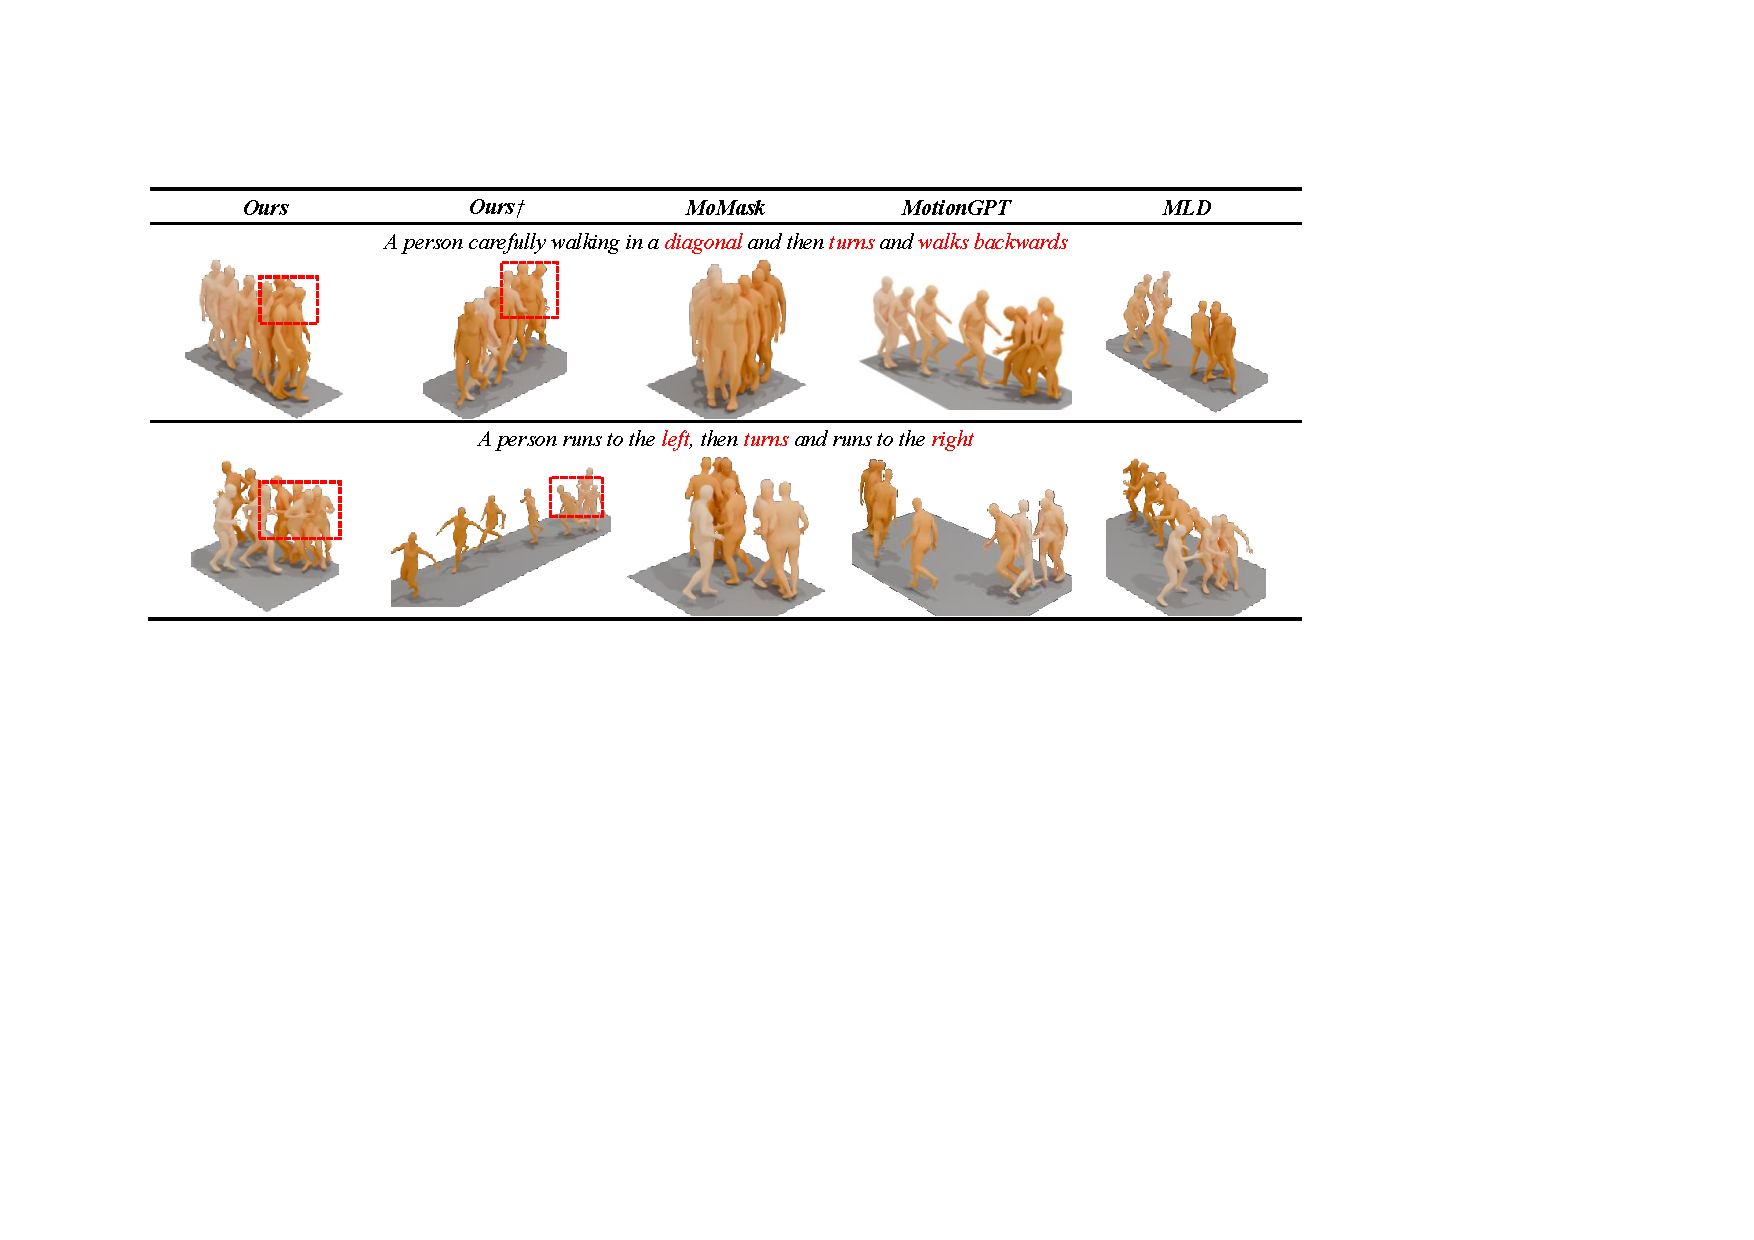
\includegraphics[width=0.95\linewidth]{fig_motion_Director/vis_7.pdf}
    \caption{Comparison results with other SOTA methods are provided. MotionDirector demonstrates a markedly superior capability in perceiving motion direction compared to other approaches. In the first sequence (row one), the diagonal walk, turn, and backward movement are captured with high fidelity. In the second sequence (row two), coordination is improved compared to MLD, and accuracy and temporal coherence surpass those of MoMask and MotionGPT. Our${\dag}$ denotes that video guidance was not provided during inference, and motion generation relied solely on the text input.
}
    \label{fig:Qualitative experimental on text-to-motion_MotionDirector.}
\end{figure*}
A further comparison is conducted between MotionDirector and recent text-to-motion methods including MoMask, MotionGPT, and MLD in the absence of video guidance. As shown in Fig.~\ref{fig:Qualitative experimental on text-to-motion_MotionDirector.}, MotionDirector produces motions that are more faithful and coherent, better reflecting directional and temporal cues described in the text. The results display smoother motion trajectories and finer-grained alignment with the textual instructions, while also surpassing MLD in coordination and continuity.

% These results highlight MotionDirector’s superior capacity to understand spatial directionality and motion order even when relying solely on text input, confirming the robustness of our DUET fusion and DASH loss design.



\subparagraph{Qualitative Evaluation on Text to Motion Generation}
\begin{figure}[htbp]
    \centering
    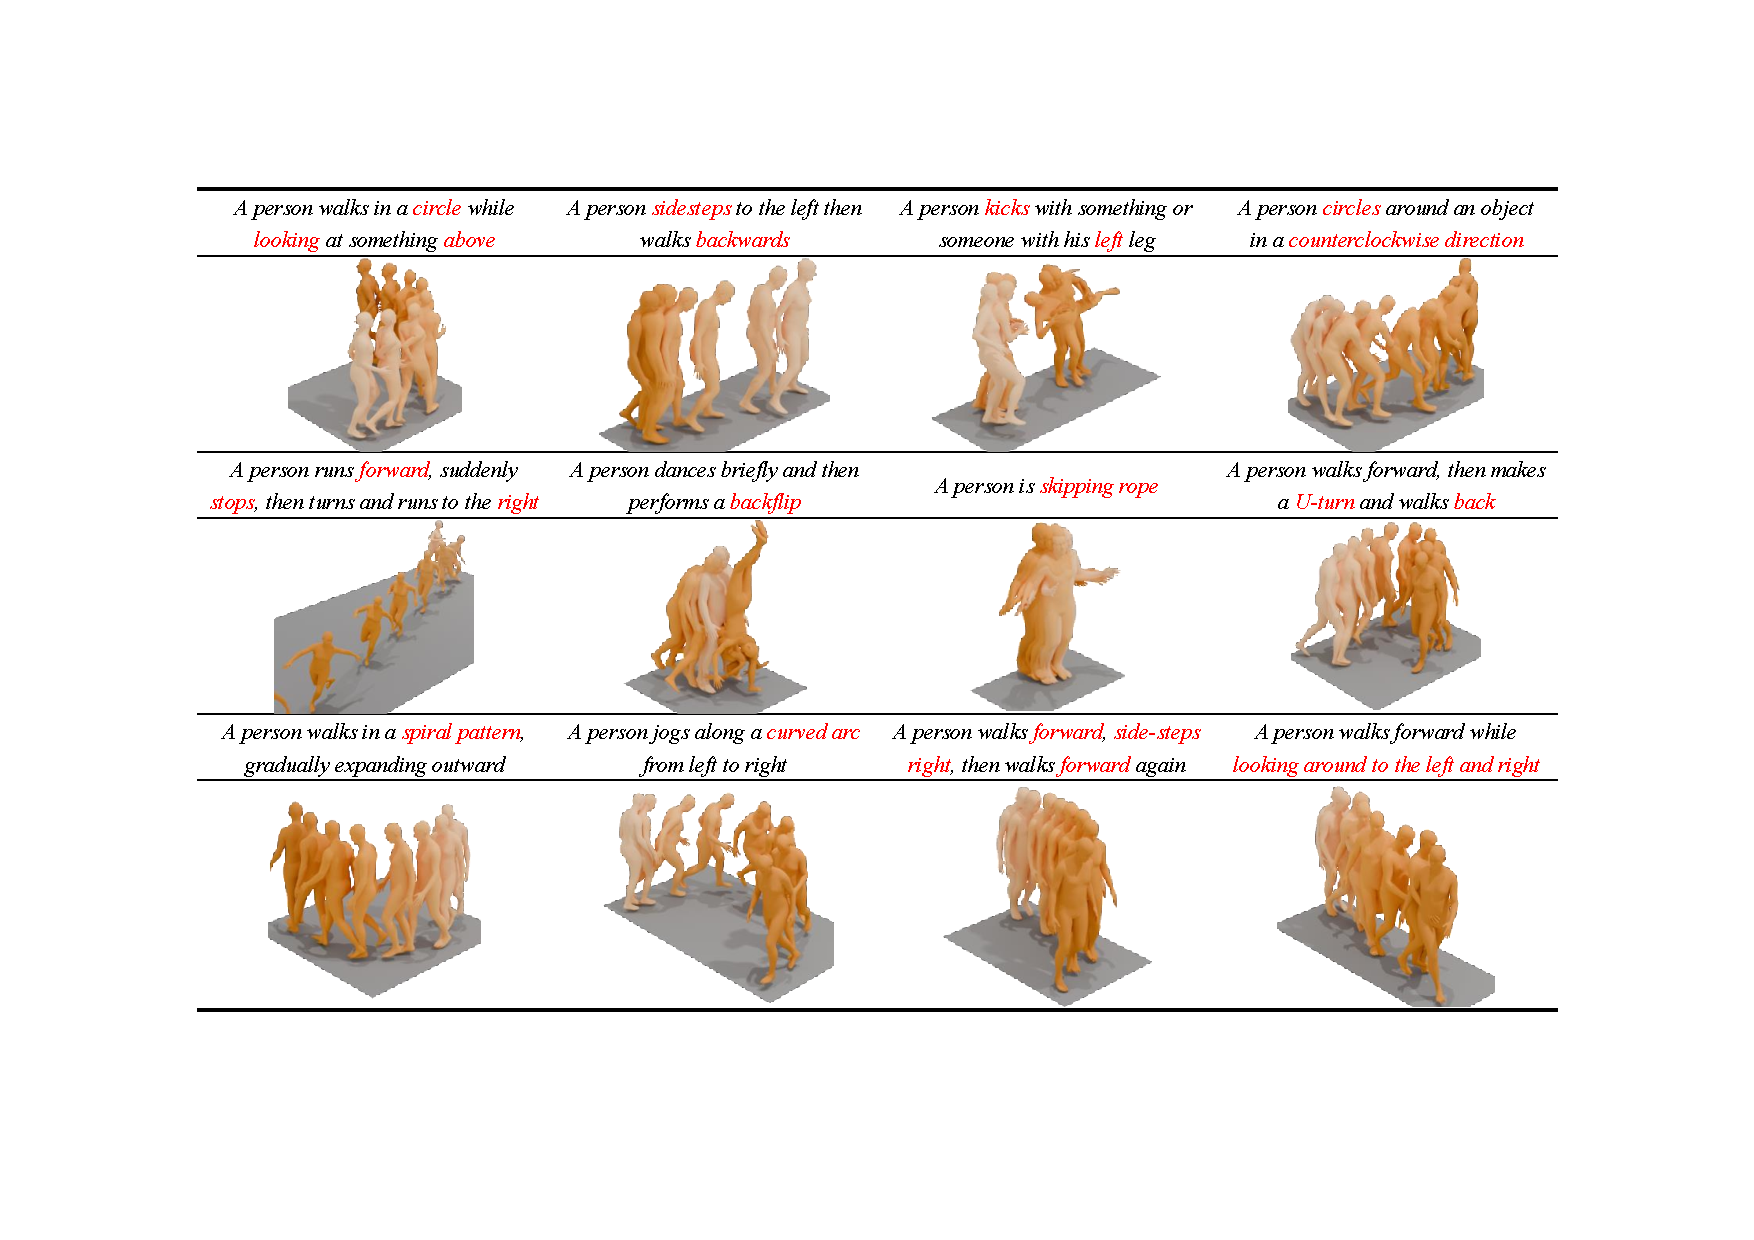
\includegraphics[width=1\linewidth]{fig_motion_Director/visual.pdf}
    \caption{More qualitative experimental results on MotionDirector. These examples cover a variety of challenging textual descriptions, involving complex action compositions and directional changes. MotionDirector is capable of generating motion sequences at a rate of approximately 199.61 poses per second during inference.}
    \label{fig:Qualitative Experimental Results}
\end{figure}
These examples cover a variety of challenging textual descriptions, involving complex action compositions and directional changes, see Fig.~\ref{fig:Qualitative Experimental Results}. By directly comparing the input text with the corresponding generated motion sequences, we can clearly observe the model’s capability to understand semantic intent, capture motion details, and maintain temporal coherence. These visual results not only demonstrate the model’s precise response to natural language instructions but also highlight its strength in producing natural, coherent, and semantically consistent human motions.


% \subparagraph{Qualitative Ablation on Video-Guided Motion Generation.}

\subparagraph{Evaluation of Generalization on Unseen Real-World Videos}
To rigorously evaluate real-world applicability and generalization ability, real-life videos are selected from the reference \cite{dong2020motion}, none of which appear during training or are included in the dataset. These videos are preprocessed and carefully trimmed into the input format required by MotionDirector. The selected samples feature several representative and high-difficulty actions, such as ballet spins, baseball pitching, hitting an incoming baseball with a bat, and golf swings (see Fig.~\ref{fig:real-world videos involving complex actions}). This evaluation serves as a strong qualitative test of the ability to handle complex real-world motion scenarios.


In the golf swing sequence, the generated motion precisely captures the smooth and continuous rotation of the torso, faithfully reflecting the arc of movement characteristic of a real swing. In the baseball throwing action, the model vividly illustrates the dynamic coordination between body rotation and arm extension, effectively conveying the power and fluidity of the throwing motion. When simulating the action of hitting a baseball with a bat, the model successfully reproduces the complete process, including lifting the bat overhead, swinging it clockwise, and making contact with the ball. In the case of the ballet turn, the model demonstrates a clear understanding of the structural subtleties of the movement, accurately portraying the dancer’s posture as they balance on one foot and rotate their body with grace. These results collectively highlight the model’s capability to generate realistic, coherent, and diverse human motions across a wide range of complex actions.

\begin{figure}[t]
    \centering
    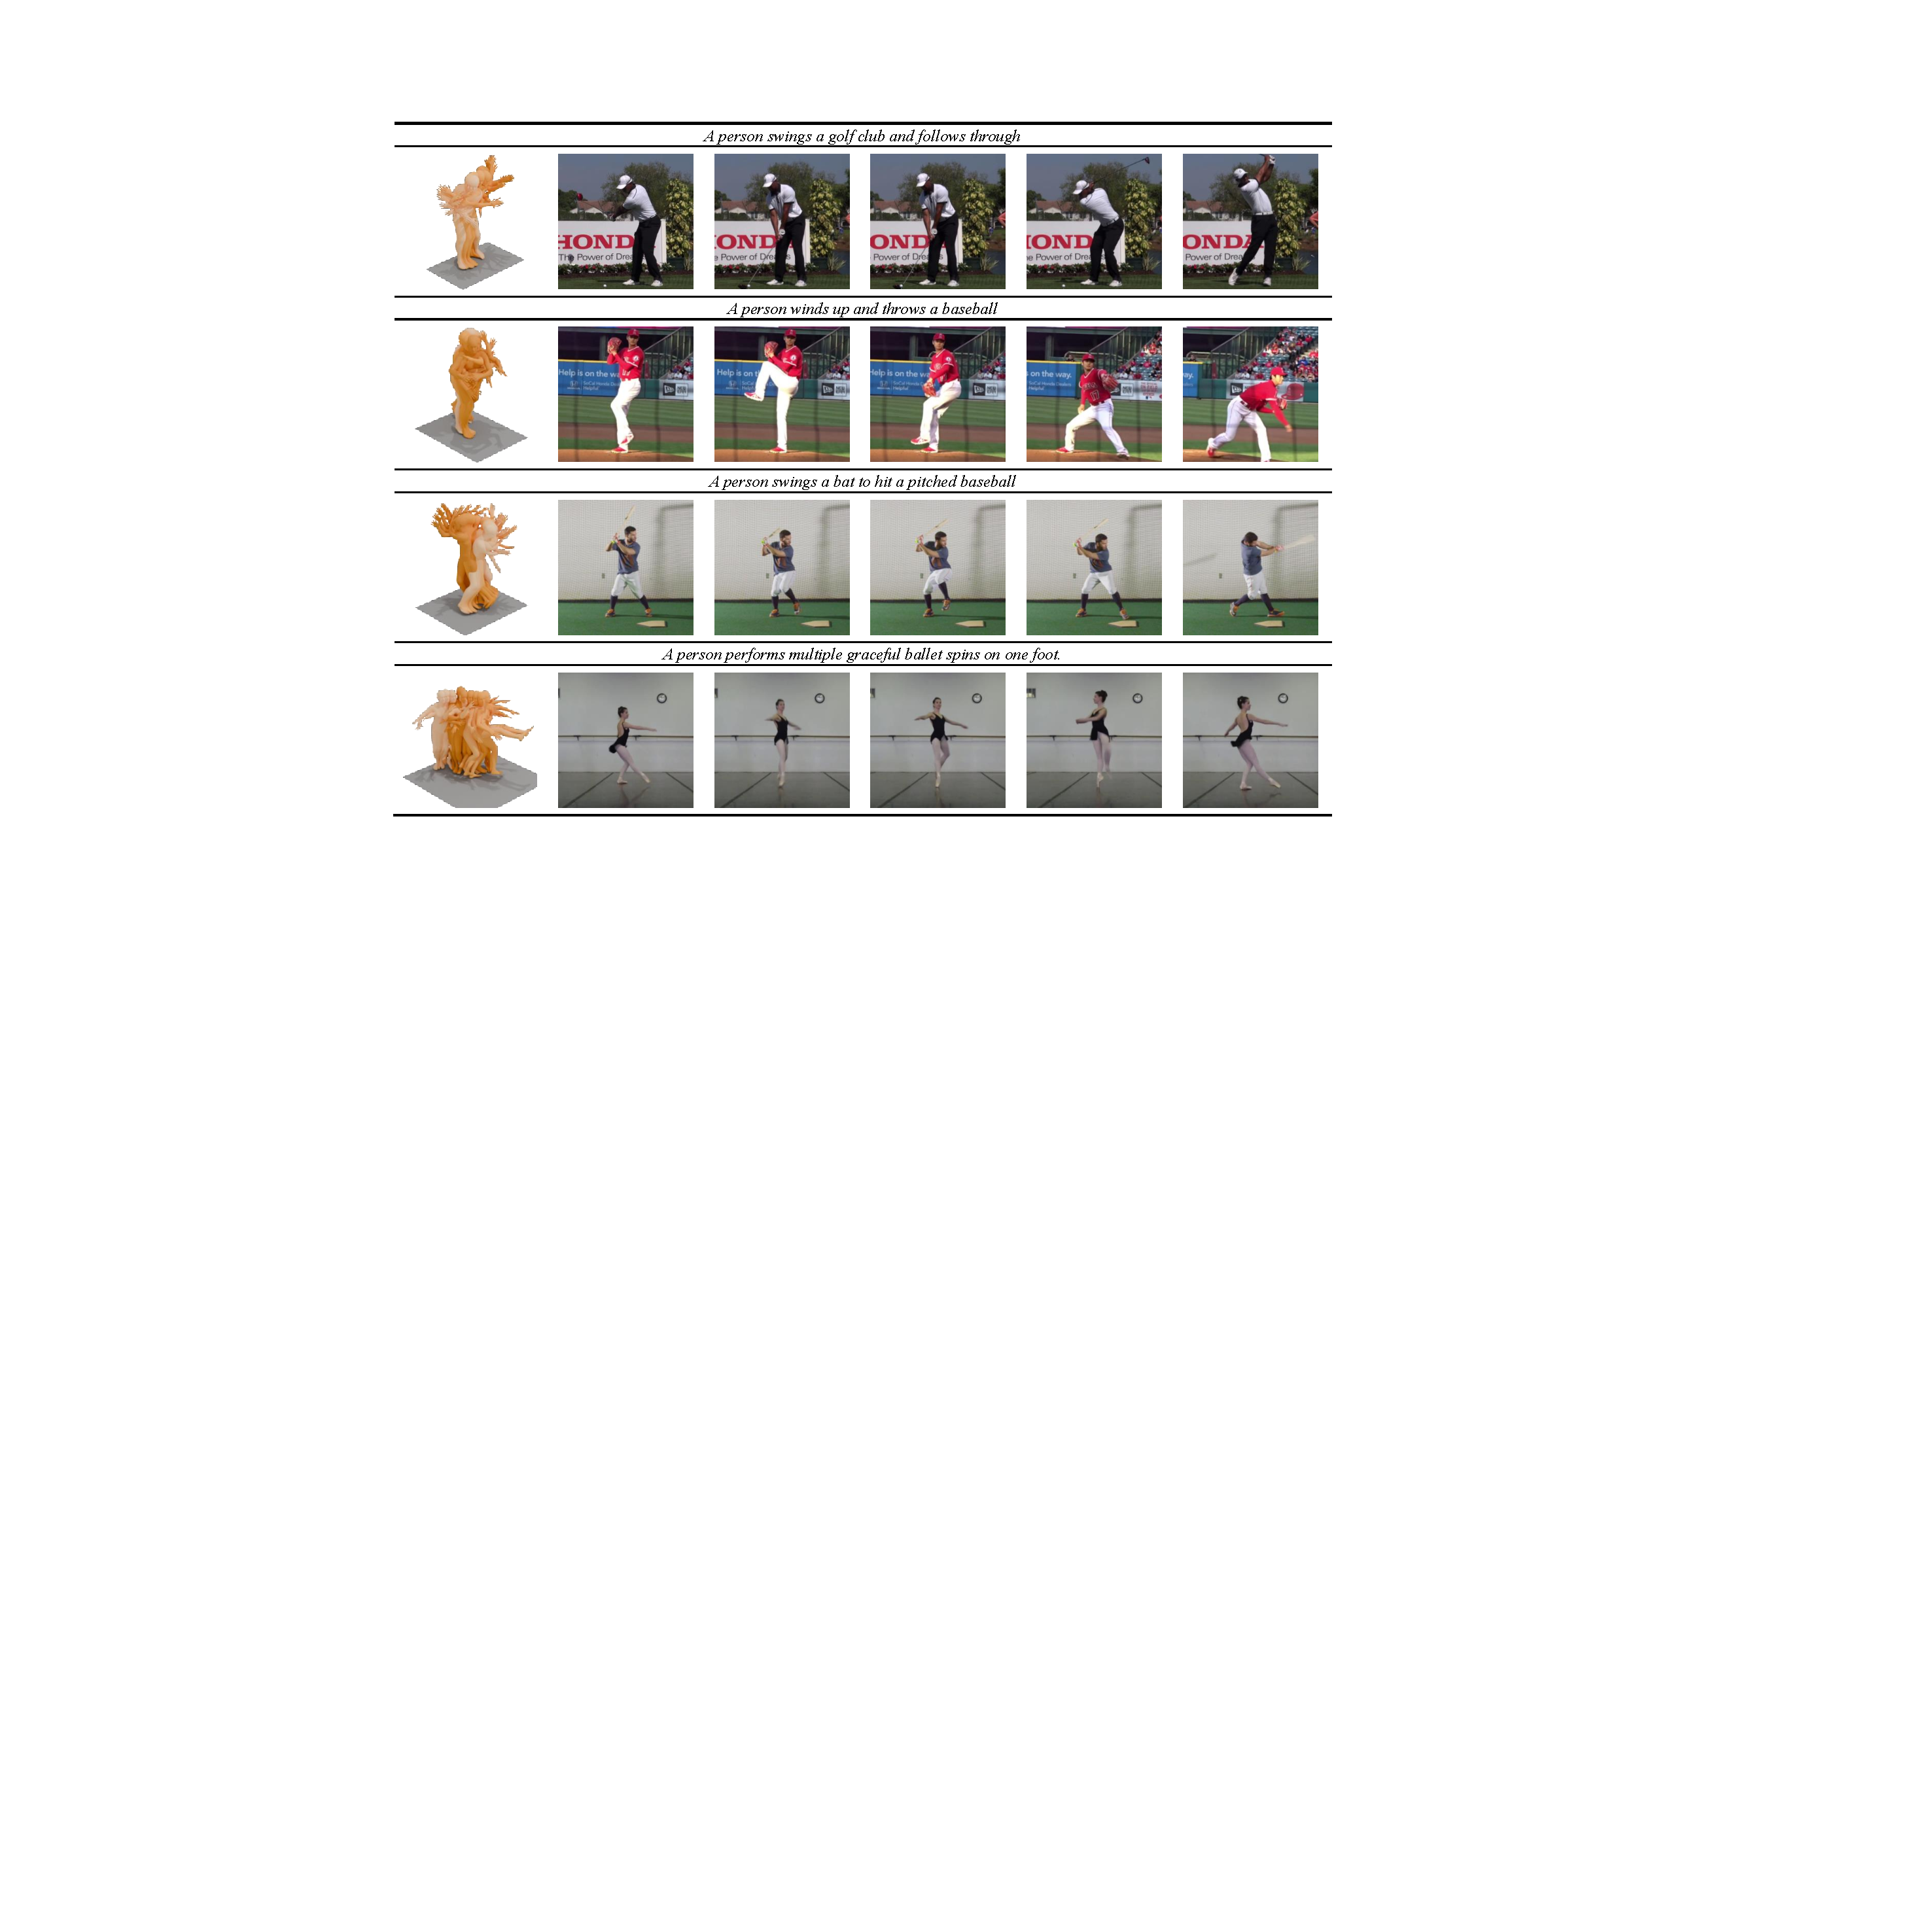
\includegraphics[width=1\linewidth]{fig_motion_Director/unseen_videos.pdf}
    \caption{Qualitative results of model-generated motions for real-world videos involving complex actions. The examples include ballet spins, baseball pitching, hitting an incoming baseball with a bat, and golf swings. Although the model was never exposed to these specific videos during training, it successfully produces semantically consistent and physically plausible motions, demonstrating its ability to generalize to unseen real-world inputs.}
    \label{fig:real-world videos involving complex actions}
\end{figure}

In the table, the first column presents the motion sequences generated by our model. The accompanying text above each sequence is a manually written description based on the corresponding video content. The remaining five columns display the reference frames, which are sampled from the original real-life video at evenly spaced intervals.

\subsubsection{Ablation Studies}

\begin{table}[t]
\centering
\scriptsize
\setlength{\tabcolsep}{4pt}  % 稍微放宽列距
\renewcommand{\arraystretch}{0.6}
\begin{tabular}{l|c|c|c}
\toprule
\textbf{Method} & \textbf{R-Top 3 ↑} & \textbf{FID ↓} & \textbf{MM Dist ↓} \\
\midrule
Real-filtering    & $0.772^{\pm.002}$ & $0.002^{\pm.000}$ & $2.954^{\pm.010}$ \\ \midrule
Concat      & $0.742^{\pm.003}$ & $0.192^{\pm.012}$ & $3.296^{\pm.010}$ \\
\hspace*{1em} + Cross-Attn   & $0.684^{\pm.002}$ & $0.707^{\pm.024}$ & $3.652^{\pm.010}$ \\ \midrule
Concat       & $0.742^{\pm.003}$ & $0.192^{\pm.012}$ & $3.296^{\pm.010}$ \\
\hspace*{1em} + FFT         & $0.726^{\pm.003}$ & $0.364^{\pm.012}$ & $3.392^{\pm.010}$ \\ \midrule
Concat       & $0.742^{\pm.003}$ & $0.192^{\pm.012}$ & $3.296^{\pm.010}$ \\
\hspace*{1em} + DMM   & $0.749^{\pm.002}$ & $0.131^{\pm.024}$ & $3.132^{\pm.010}$ \\ \midrule
Concat      & $0.742^{\pm.003}$ & $0.192^{\pm.012}$ & $3.296^{\pm.010}$ \\
\hspace*{1em} + Self-Attn    & $0.714^{\pm.003}$ & $0.222^{\pm.012}$ & $3.314^{\pm.010}$ \\ 
\hspace*{2em} + DMM      & $0.721^{\pm.003}$ & $0.228^{\pm.012}$ & $3.320^{\pm.010}$ \\ \midrule
Hadamard Product           & $0.741^{\pm.003}$ & $0.243^{\pm.012}$ & $3.219^{\pm.010}$ \\
\hspace*{1em} + FFT         & $0.743^{\pm.003}$ & $0.292^{\pm.012}$ & $3.226^{\pm.010}$ \\
\hspace*{2em} + DMM      & $0.727^{\pm.003}$ & $0.280^{\pm.012}$ & $3.311^{\pm.010}$ \\  \midrule
Element-Wise Add       & $0.747^{\pm.003}$ & $0.168^{\pm.012}$ & $3.388^{\pm.010}$ \\
\hspace*{1em} + FFT         & $0.743^{\pm.003}$ & $0.204^{\pm.012}$ & $3.256^{\pm.010}$ \\ \midrule
Element-Wise Add       & $0.747^{\pm.003}$ & $0.168^{\pm.012}$ & $3.388^{\pm.010}$ \\
\hspace*{1em}+ DMM         & $0.750^{\pm.003}$ & $0.204^{\pm.012}$ & $3.256^{\pm.010}$ \\ 
\hspace*{2em} + FFT & $0.744^{\pm.003}$ & $0.254^{\pm.012}$ & $3.299^{\pm.010}$ \\ \midrule
Element-Wise Add       & $0.747^{\pm.003}$ & $0.168^{\pm.012}$ & $3.388^{\pm.010}$ \\
\hspace*{1em}+ DMM         & $0.750^{\pm.003}$ & $0.204^{\pm.012}$ & $3.256^{\pm.010}$ \\ 
\hspace*{1em}+ FFT & $0.750^{\pm.003}$ & $0.163^{\pm.012}$ & $3.178^{\pm.010}$ \\ 
\hspace*{1em}+ Identity     & $0.752^{\pm.003}$ & $0.147^{\pm.012}$ & $3.124^{\pm.010}$ \\ 
\hspace*{1em}+ Conv (DUET)  & \bm{$0.755^{\pm.003}$} & \bm{$0.101^{\pm.024}$} & \bm{$3.087^{\pm.010}$} \\
\bottomrule
\end{tabular}
\caption{Performance comparison of different multimodal fusion strategies. Table indentation denotes the sequential integration of modules, with each indented block representing a component appended downstream within the overall architecture. The top results in each column are highlighted with 
\textbf{bold}.}
\label{tab:fusion_strategies}
\end{table}

\begin{table}[t]
\centering
\footnotesize
\setlength{\tabcolsep}{4pt}  % 稍微放宽列距
\renewcommand{\arraystretch}{0.7}
\begin{tabular}{l|c|c|c}
\toprule
\textbf{} & \textbf{R-Top 3 ↑} & \textbf{FID ↓} & \textbf{MM Dist ↓} \\
\midrule
Real             & $0.797^{\pm.003}$ & $0.002^{\pm.000}$ & $2.974^{\pm.008}$ \\
\midrule
Baseline         & $0.772^{\pm.002}$ & $0.473^{\pm.024}$ & $3.196^{\pm.010}$ \\
+ Filtering      & $0.734^{\pm.002}$ & $0.396^{\pm.024}$ & $3.156^{\pm.010}$ \\
\midrule
Real-filtering   & $0.772^{\pm.002}$ & $0.002^{\pm.000}$ & $2.954^{\pm.010}$ \\
\midrule
+ Video          & $0.742^{\pm.003}$ & $0.192^{\pm.012}$ & $3.296^{\pm.010}$ \\
+ DUET           & $0.755^{\pm.003}$ & $0.101^{\pm.024}$ & \bm{$3.087^{\pm.010}$} \\
+ DASH Loss          & \bm{$0.764^{\pm.003}$} & \bm{$0.084^{\pm.012}$} & $3.089^{\pm.010}$ \\
\bottomrule
\end{tabular}
\caption{Evaluation on each component. The best results per column are highlighted in \textbf{Bold}.}
\label{tab:ablation_no_mm}
\end{table}


\paragraph{Evaluation on Multimodal Fusion Strategies}
This section presents a quantitative comparison of various multimodal fusion strategies, as shown in Table~\ref{tab:fusion_strategies}. To isolate the effects of the core components, experiments are conducted on the filtered HumanML3D dataset, with the DASH Loss intentionally excluded from the training objective at this stage. Several commonly used fusion strategies are first evaluated, and element-wise addition is found to consistently achieve superior performance across multiple metrics.

Subsequently, serial compositions are explored by sequentially appending modules such as Cross-Attention, FFT, and Similarity guidance. However, the results indicate that most of these combinations fail to deliver performance gains. A possible explanation is that such serial structures may lead the model to overemphasize one modality or information stream while neglecting others. Motivated by this observation, a novel design is proposed that builds upon element-wise addition by introducing four parallel branches, each focusing on a distinct type of supplementary information. The final fusion module, DUET, demonstrates clear advantages over existing methods, achieving an R-Precision Top-3 of 0.755 and an FID of 0.101, thereby validating the effectiveness of the proposed fusion architecture in integration quality.


\paragraph{Evaluation on Each Component}
This section outlines the ablation study process, as shown in Table~\ref{tab:ablation_no_mm}. A video-based motion dataset is first constructed, in which various issues such as motion inconsistency and severe action errors are observed. To address these problems, a data cleaning strategy is designed, which is detailed in the Appendix. Using the cleaned dataset, the baseline model is re-evaluated and notable improvements are observed across several metrics. 

For conditioning, prior work is followed and concatenation-based modality fusion~\cite{chen2023executing} is adopted. This yields consistent improvements in R-Precision (Top-1/2/3), with an average increase of approximately 3.8\%, and a significant 51.52\% reduction in FID. The proposed multimodal fusion module, DUET, is then integrated into the framework, replacing the concatenation-based fusion used in earlier experiments. This results in a 47.40\% reduction in FID.

Building upon the previous experimental stages, the DASH Loss is incorporated into the training procedure. To further refine performance, Auto Guidance is applied, with the optimal configuration selected via dropout or noise search. The model achieves a final FID of 0.088, marking an order-of-magnitude improvement over baseline components. These results validate the effectiveness of the incremental design and demonstrate the additive value contributed by each module.



\paragraph{Qualitative Ablation on Video-Guided Motion Generation}

\begin{figure}[t]
    \centering
    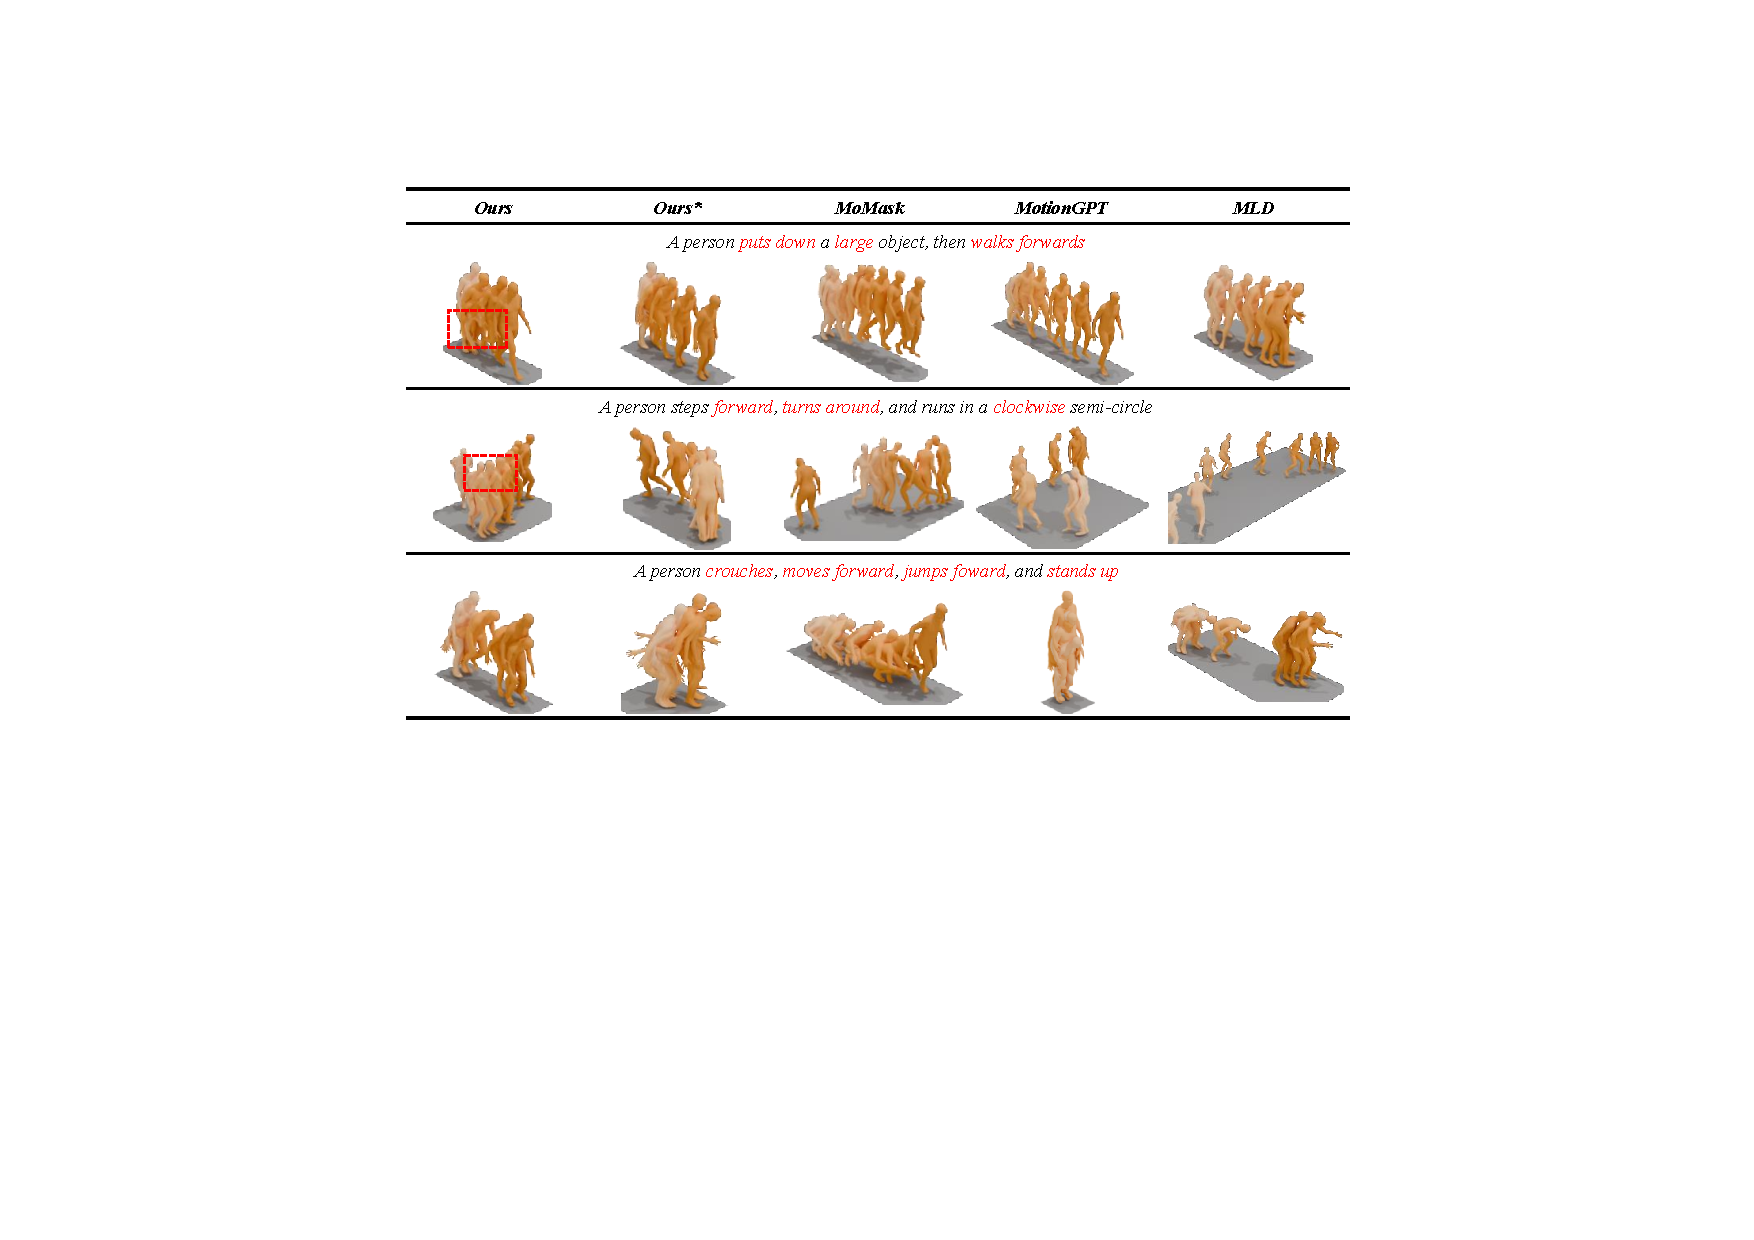
\includegraphics[width=\linewidth]{fig_motion_Director/vis_6.pdf}
    \caption{Comparison of qualitative experimental results. A qualitative comparison of MotionDirector with three methods—MoMask, MotionGPT, and MLD—is conducted. Compared to previous methods, MotionDirector generates more realistic and coherent motions, with better alignment to fine-grained language instructions such as “puts down a large object”, “turn around”, and “crouches and jumps forward”. Our* denotes an ablation variant in which video inputs are excluded during training to validate their contribution to model performance. As video information is unavailable in this setting, the DASH Loss is removed accordingly, while the other components of the DUET module, excluding DMM, are retained.
}
    \label{fig:Comparison of Qualitative Experimental Results}
\end{figure}

To deepen this comparison and isolate the contribution of video inputs, an ablation study is performed in which video inputs are excluded during training. As a result, the DASH Loss is removed due to its reliance on video information, while the remaining components of the DUET module, except for DMM, are preserved to ensure a consistent and fair evaluation. In addition, qualitative evaluations of the generated motion sequences are conducted across a diverse set of textual prompts to further assess the effectiveness of the proposed method. As shown in Fig.~\ref{fig:Comparison of Qualitative Experimental Results}, MotionDirector excels at generating realistic and semantically aligned human motions in response to complex natural language descriptions.


\paragraph{Evaluation of Hyperparameters $\lambda_{\text{DASH}}$}

\begin{table*}[t]
\centering
\scriptsize
\renewcommand{\arraystretch}{1}
\begin{tabular}{c|ccc|c|c|c|c}
\toprule
\multirow{2}{*}{\textbf{$\lambda_{\text{DASH}}$}} & \multicolumn{3}{c|}{\textbf{R Precision ↑}} & \multirow{2}{*}{\textbf{FID ↓}} & \multirow{2}{*}{\textbf{MM Dist ↓}} & \multirow{2}{*}{\textbf{Diversity →}} & \multirow{2}{*}{\textbf{MM ↑}} \\
 & Top 1 & Top 2 & Top 3 &  &  &  & \\
\midrule
Real-filtering    & $0.490^{\pm.003}$ & $0.684^{\pm.003}$ & $0.772^{\pm.002}$ & $0.002^{\pm.000}$ & $2.954^{\pm.010}$ & $9.492^{\pm.002}$ & -- \\ \midrule
0.1        & $0.474^{\pm.003}$ & $0.668^{\pm.003}$ & $0.764^{\pm.003}$ & $0.084^{\pm.012}$ & $3.089^{\pm.010}$ & $9.527^{\pm.071}$ & $2.576^{\pm.071}$ \\
0.3       & $0.466^{\pm.003}$ & $0.657^{\pm.003}$ & $0.752^{\pm.002}$ & $0.143^{\pm.024}$ & $3.169^{\pm.010}$ & $9.532^{\pm.071}$ & $2.453^{\pm.018}$ \\
0.5    & $0.469^{\pm.003}$ & $0.645^{\pm.003}$ & $0.745^{\pm.002}$ & $0.186^{\pm.024}$ & $3.280^{\pm.010}$ & $9.810^{\pm.071}$ &$2.456^{\pm.018}$ \\ 
0.7    & $0.452^{\pm.003}$ & $0.647^{\pm.003}$ & $0.743^{\pm.002}$ & $0.237^{\pm.024}$ & $3.311^{\pm.010}$ & $9.314^{\pm.071}$ & $2.412^{\pm.018}$ \\ 
0.9            & $0.443^{\pm.003}$ & $0.632^{\pm.003}$ & $0.734^{\pm.003}$ & $0.294^{\pm.012}$ & $3.324^{\pm.010}$ & $9.277^{\pm.071}$ & $2.427^{\pm.018}$ \\
1    & $0.433^{\pm.003}$ & $0.638^{\pm.003}$ & $0.732^{\pm.003}$ & $0.427^{\pm.024}$ & $3.322^{\pm.010}$ & $9.212^{\pm.071}$ & $2.563^{\pm.018}$ \\
50    & $0.345^{\pm.003}$ & $0.525^{\pm.003}$ & $0.635^{\pm.003}$ & $1.438^{\pm.024}$ & $3.997^{\pm.010}$ & $8.653^{\pm.071}$ & $2.672^{\pm.018}$ \\
100   & $0.310^{\pm.003}$ & $0.474^{\pm.003}$ & $0.600^{\pm.003}$ & $2.500^{\pm.012}$ & $4.275^{\pm.010}$ & $8.731^{\pm.071}$ & $2.654^{\pm.018}$ \\
200   & $0.159^{\pm.003}$ & $0.278^{\pm.003}$ & $0.369^{\pm.003}$ & $8.676^{\pm.012}$ & $5.660^{\pm.010}$ & $7.369^{\pm.071}$ & $2.684^{\pm.018}$ \\
300   & $0.039^{\pm.003}$ & $0.058^{\pm.003}$ & $0.099^{\pm.003}$ & $14.676^{\pm.012}$ & $7.320^{\pm.010}$ & $5.832^{\pm.071}$ & $2.953^{\pm.018}$ \\
\bottomrule
\end{tabular}
\caption{Parameter Study on $\lambda_{\text{DASH}}$. $\uparrow$ indicates higher is better, and $\downarrow$ indicates lower is better.}
\label{tab:Hyperparameters_1}
\end{table*}


A detailed analysis and discussion on the range of values for the hyperparameter $\lambda_{\text{DASH}}$ is conducted to understand its influence on model performance, as shown in Table~\ref{tab:Hyperparameters_1}. Experimental results reveal a clear trend: while introducing the DASH Loss with a moderate weight can effectively improve the quality and consistency of motion generation, setting $\lambda_{\text{DASH}}$ too high leads to a noticeable performance degradation. This is likely because an excessively strong DASH Loss may overpower other learning signals, causing the model to overfit to the video features and thereby reducing its generalization ability, especially when video inputs are unavailable at inference time.


\paragraph{Study on Auto-Guidance Mechanism Weights $\omega$}
Automatic guidance identifies and corrects potential errors by measuring the discrepancy between the predictions of a strong model and a weaker one, thereby amplifying adjustments in a more favorable direction. When the two models produce similar outputs, the perturbation is negligible; however, when they diverge, the difference serves as an approximate signal toward a better sample distribution~\cite{karras2024guiding}. To investigate the effectiveness of Auto Guidance under multimodal settings, an ablation study is conducted on two key factors: the modality-specific influence weights $\omega$ and the perturbation strategies—dropout and input noise. Specifically, three groups of settings are evaluated:

\begin{itemize}
    \item \textbf{Dropout-only} configurations: $\mathcal{D}_1$ and $\mathcal{D}_2$ represent feature-level dropout rates (e.g., $5\%$ and $10\%$) applied post-hoc to the base model. The guidance model operates using these degraded features to mimic a weaker model variant.
    
    \item \textbf{Noise-only} configurations: $\epsilon_1$ and $\epsilon_2$ indicate different levels of Gaussian noise (e.g., standard deviation increments of $5\%$ and $10\%$) added to the input embeddings. This simulates corrupted conditions to encourage robust generation.
    
    % \item \textbf{Combined perturbation} configurations: Dropout and noise are jointly applied to construct $\mathcal{D}_1 + \epsilon_1$ and $\mathcal{D}_2 + \epsilon_2$, enabling complementary exploration of feature and embedding-level degradation.
\end{itemize}

\begin{table*}[t]
\centering
\scriptsize
\renewcommand{\arraystretch}{1}
\begin{tabular}{cc|ccc|c|c|c|c}
\toprule
\multirow{2}{*}{\textbf{$\mathcal{D}_1$}}& \multirow{2}{*}{\textbf{$\omega$}} & \multicolumn{3}{c|}{\textbf{R Precision ↑}} & \multirow{2}{*}{\textbf{FID ↓}} & \multirow{2}{*}{\textbf{MM Dist ↓}} & \multirow{2}{*}{\textbf{Diversity →}} & \multirow{2}{*}{\textbf{MM ↑}} \\
& & Top 1 & Top 2 & Top 3 &  &  &  & \\
\midrule
Real-filtering   & -- & $0.490^{\pm.003}$ & $0.684^{\pm.003}$ & $0.772^{\pm.002}$ & $0.002^{\pm.000}$ & $2.954^{\pm.010}$ & $9.492^{\pm.002}$ & -- \\ \midrule
\multirow{5}{*}{\textbf{5\%}}
& 0.75  & $0.462^{\pm.005}$ & $0.651^{\pm.006}$ & $0.742^{\pm.005}$ & $0.121^{\pm.022}$ & $3.095^{\pm.014}$ & $9.320^{\pm.077}$ & $2.543^{\pm.065}$ \\
& 1.00 & $0.469^{\pm.004}$ & $0.657^{\pm.004}$ & $0.744^{\pm.003}$ & $0.142^{\pm.018}$ & $3.082^{\pm.009}$ & $9.355^{\pm.069}$ & $2.580^{\pm.073}$ \\
& 1.25  & $0.474^{\pm.003}$ & $0.668^{\pm.003}$ & $0.764^{\pm.003}$ & $0.084^{\pm.012}$ & $3.089^{\pm.010}$ & $9.527^{\pm.071}$ & $2.576^{\pm.071}$ \\
& 1.50  & $0.463^{\pm.005}$ & $0.654^{\pm.005}$ & $0.745^{\pm.005}$ & $0.102^{\pm.024}$ & $3.100^{\pm.015}$ & $9.310^{\pm.073}$ & $2.598^{\pm.068}$ \\
& 1.75 & $0.469^{\pm.004}$ & $0.657^{\pm.004}$ & $0.749^{\pm.003}$ & $0.097^{\pm.018}$ & $3.082^{\pm.009}$ & $9.355^{\pm.069}$ & $2.513^{\pm.073}$ \\
\midrule

\multirow{2}{*}{\textbf{$\mathcal{D}_2$}}& \multirow{2}{*}{\textbf{$\omega$}} & \multicolumn{3}{c|}{\textbf{R Precision ↑}} & \multirow{2}{*}{\textbf{FID ↓}} & \multirow{2}{*}{\textbf{MM Dist ↓}} & \multirow{2}{*}{\textbf{Diversity →}} & \multirow{2}{*}{\textbf{MM ↑}} \\
& & Top 1 & Top 2 & Top 3 &  &  &  & \\
\midrule

\multirow{5}{*}{\textbf{10\%}} 
& 0.75  & $0.468^{\pm.004}$ & $0.662^{\pm.003}$ & $0.755^{\pm.004}$ & $0.102^{\pm.020}$ & $3.090^{\pm.012}$ & $9.480^{\pm.075}$ & $2.572^{\pm.068}$ \\
& 1.0 & $0.473^{\pm.003}$ & $0.666^{\pm.003}$ & $0.758^{\pm.003}$ & $0.132^{\pm.019}$ & $3.082^{\pm.011}$ & $9.503^{\pm.070}$ & $2.579^{\pm.071}$ \\
& 1.25  & $0.474^{\pm.003}$ & $0.668^{\pm.003}$ & $0.760^{\pm.003}$ & $0.153^{\pm.018}$ & $3.089^{\pm.010}$ & $9.510^{\pm.072}$ & $2.580^{\pm.069}$ \\
& 1.50 & $0.471^{\pm.004}$ & $0.663^{\pm.003}$ & $0.756^{\pm.004}$ & $0.113^{\pm.022}$ & $3.088^{\pm.011}$ & $9.495^{\pm.071}$ & $2.575^{\pm.070}$ \\
& 1.75  & $0.469^{\pm.003}$ & $0.661^{\pm.004}$ & $0.753^{\pm.003}$ & $0.323^{\pm.021}$ & $3.085^{\pm.010}$ & $9.485^{\pm.073}$ & $2.570^{\pm.068}$ \\
\midrule

\multirow{2}{*}{\textbf{$\epsilon_1$}}& \multirow{2}{*}{\textbf{$\omega$}} & \multicolumn{3}{c|}{\textbf{R Precision ↑}} & \multirow{2}{*}{\textbf{FID ↓}} & \multirow{2}{*}{\textbf{MM Dist ↓}} & \multirow{2}{*}{\textbf{Diversity →}} & \multirow{2}{*}{\textbf{MM ↑}} \\
& & Top 1 & Top 2 & Top 3 &  &  &  & \\
\midrule

\multirow{5}{*}{\textbf{5\%}} 
& 0.75  & $0.458^{\pm.005}$ & $0.645^{\pm.005}$ & $0.735^{\pm.004}$ & $0.102^{\pm.023}$ & $3.095^{\pm.013}$ & $9.315^{\pm.074}$ & $2.727^{\pm.069}$ \\
& 1.00 & $0.464^{\pm.004}$ & $0.650^{\pm.004}$ & $0.740^{\pm.004}$ & $0.132^{\pm.022}$ & $3.090^{\pm.012}$ & $9.345^{\pm.070}$ & $2.575^{\pm.070}$ \\
& 1.25  & $0.467^{\pm.004}$ & $0.653^{\pm.003}$ & $0.743^{\pm.003}$ & $0.231^{\pm.020}$ & $3.088^{\pm.011}$ & $9.355^{\pm.071}$ & $2.576^{\pm.068}$ \\
& 1.50 & $0.466^{\pm.004}$ & $0.654^{\pm.004}$ & $0.745^{\pm.004}$ & $0.173^{\pm.021}$ & $3.090^{\pm.011}$ & $9.350^{\pm.069}$ & $2.573^{\pm.071}$ \\
& 1.75  & $0.462^{\pm.004}$ & $0.648^{\pm.004}$ & $0.737^{\pm.004}$ & $0.152^{\pm.023}$ & $3.092^{\pm.012}$ & $9.338^{\pm.072}$ & $2.571^{\pm.070}$ \\ \midrule

\multirow{2}{*}{\textbf{$\epsilon_1$}}& \multirow{2}{*}{\textbf{$\omega$}} & \multicolumn{3}{c|}{\textbf{R Precision ↑}} & \multirow{2}{*}{\textbf{FID ↓}} & \multirow{2}{*}{\textbf{MM Dist ↓}} & \multirow{2}{*}{\textbf{Diversity →}} & \multirow{2}{*}{\textbf{MM ↑}} \\
& & Top 1 & Top 2 & Top 3 &  &  &  & \\
\midrule

\multirow{5}{*}{\textbf{10\%}} 
& 0.75  & $0.446^{\pm.005}$ & $0.643^{\pm.005}$ & $0.726^{\pm.004}$ & $0.143^{\pm.023}$ & $3.135^{\pm.013}$ & $9.853^{\pm.074}$ & $2.767^{\pm.069}$ \\
& 1.00 & $0.461^{\pm.004}$ & $0.643^{\pm.004}$ & $0.737^{\pm.004}$ & $0.134^{\pm.022}$ & $3.103^{\pm.012}$ & $9.338^{\pm.070}$ & $2.687^{\pm.070}$ \\
& 1.25  & $0.465^{\pm.004}$ & $0.646^{\pm.003}$ & $0.739^{\pm.003}$ & $0.253^{\pm.020}$ & $3.132^{\pm.011}$ & $9.285^{\pm.071}$ & $2.523^{\pm.068}$ \\
& 1.50 & $0.461^{\pm.004}$ & $0.649^{\pm.004}$ & $0.742^{\pm.004}$ & $0.198^{\pm.021}$ & $3.138^{\pm.011}$ & $9.380^{\pm.069}$ & $2.543^{\pm.071}$ \\
& 1.75  & $0.454^{\pm.004}$ & $0.643^{\pm.004}$ & $0.737^{\pm.004}$ & $0.182^{\pm.023}$ & $3.132^{\pm.012}$ & $9.398^{\pm.072}$ & $2.592^{\pm.070}$ \\

\bottomrule
\end{tabular}
\caption{Parameter Study on $\omega$ and Dropout. $\uparrow$ indicates higher is better, and $\downarrow$ lower is better.}
\label{tab:Hyperparameters_2}
\end{table*}

Across all groups, the weighting parameter $\omega$ is systematically swept to determine optimal influence magnitudes for each degraded condition, as shown in Table~\ref{tab:Hyperparameters_2}. Dropout-only perturbation is observed to lead to more stable training compared to noise-based alternatives. This is likely because dropout removes a subset of the conditional inputs while preserving the semantic consistency of the remaining tokens. In contrast, noise injection distorts the content of the condition embeddings, potentially introducing semantic ambiguity and interfering with effective supervision. Moreover, dropout provides a natural curriculum for gradually increasing conditional strength, which is more conducive to stable convergence.

\paragraph{Evaluation of Loss Function}
A comparative study is conducted between the proposed DASH Loss and the infoNCE loss to evaluate their impact on motion generation quality. While cosine loss encourages alignment between motion and video features at the token level, it lacks explicit structural regularization and fails to preserve the internal relationships within each modality. In contrast, DASH Loss incorporates both token-level similarity and pairwise structural consistency, promoting better semantic grounding and distribution alignment. As shown in Table~\ref{tab:comparison_loss}, improved performance across all key metrics is achieved, demonstrating the effectiveness of DASH Loss in bridging the modality gap and enhancing generation quality.


\begin{table*}[t]
\centering
\scriptsize
\renewcommand{\arraystretch}{1}
\setlength{\tabcolsep}{4.5pt}  % 稍微放宽列距
\begin{tabular}{l|ccc|c|c|c|c}
\toprule
\multirow{2}{*}{\textbf{Method}} & \multicolumn{3}{c|}{\textbf{R Precision ↑}} & \multirow{2}{*}{\textbf{FID ↓}} & \multirow{2}{*}{\textbf{MM Dist ↓}} & \multirow{2}{*}{\textbf{Diversity →}} & \multirow{2}{*}{\textbf{MM ↑}} \\
 & Top 1 & Top 2 & Top 3 &  &  &  & \\
\midrule
Real-filtering    & $0.490^{\pm.003}$ & $0.684^{\pm.003}$ & $0.772^{\pm.002}$ & $0.002^{\pm.000}$ & $2.954^{\pm.010}$ & $9.492^{\pm.002}$ & -- \\ \midrule
infoNCE loss       & $0.458^{\pm.003}$ & $0.642^{\pm.003}$ & $0.746^{\pm.003}$ & $1.773^{\pm.012}$ & $3.131^{\pm.010}$ & $9.583^{\pm.071}$ & $2.632^{\pm.071}$ \\ 
Token-wise Margin Loss       & $0.473^{\pm.003}$ & $0.665^{\pm.003}$ & $0.756^{\pm.003}$ & $0.096^{\pm.012}$ & $3.102^{\pm.010}$ & $9.534^{\pm.071}$ & $2.535^{\pm.071}$ \\ \midrule
DASH Loss       & $0.474^{\pm.003}$ & $0.668^{\pm.003}$ & $0.762^{\pm.003}$ & $0.084^{\pm.012}$ & $3.089^{\pm.010}$ & $9.527^{\pm.071}$ & $2.576^{\pm.071}$ \\ 

\bottomrule
\end{tabular}
\caption{ 
Evaluation of Loss Function. $\uparrow$ indicates higher is better, $\downarrow$ indicates lower is better, and $\rightarrow$ indicates closer is better. 
}
\label{tab:comparison_loss}
\end{table*}

\paragraph{Multimodal Fusion Strategies}
The complete results of the ablation studies on multimodal fusion strategies are provided for reference, as shown in Table~\ref{tab:fusion_strategies_full}. These supplementary results offer a more comprehensive understanding of how different fusion methods perform under various conditions and further support the analysis of the sources contributing to performance improvements.


\begin{table*}[t]
\centering
\tiny
\renewcommand{\arraystretch}{0.8}
\begin{tabular}{l|ccc|c|c|c|c}
\toprule
\multirow{2}{*}{\textbf{Method}} & \multicolumn{3}{c|}{\textbf{R Precision ↑}} & \multirow{2}{*}{\textbf{FID ↓}} & \multirow{2}{*}{\textbf{MM Dist ↓}} & \multirow{2}{*}{\textbf{Diversity →}} & \multirow{2}{*}{\textbf{MM ↑}} \\
 & Top 1 & Top 2 & Top 3 &  &  &  & \\
\midrule
Real-filtering    & $0.490^{\pm.003}$ & $0.684^{\pm.003}$ & $0.772^{\pm.002}$ & $0.002^{\pm.000}$ & $2.954^{\pm.010}$ & $9.492^{\pm.002}$ & -- \\ \midrule
Concat      & $0.463^{\pm.003}$ & $0.652^{\pm.003}$ & $0.742^{\pm.003}$ & $0.192^{\pm.012}$ & $3.296^{\pm.010}$ & $9.687^{\pm.071}$ & $2.412^{\pm.071}$ \\
\hspace*{1em} + Cross-Attn   & $0.380^{\pm.002}$ & $0.568^{\pm.002}$ & $0.684^{\pm.002}$ & $0.707^{\pm.024}$ & $3.652^{\pm.010}$ & $9.308^{\pm.071}$ & \bm{$3.276^{\pm.018}$} \\ \midrule
Concat       & $0.463^{\pm.003}$ & $0.652^{\pm.003}$ & $0.742^{\pm.003}$ & $0.192^{\pm.012}$ & $3.296^{\pm.010}$ & $9.687^{\pm.071}$ & $2.412^{\pm.071}$ \\
\hspace*{1em} + FFT         & $0.430^{\pm.003}$ & $0.626^{\pm.003}$ & $0.726^{\pm.003}$ & $0.364^{\pm.012}$ & $3.392^{\pm.010}$ & $9.703^{\pm.071}$ & $2.640^{\pm.071}$ \\ \midrule
Concat       & $0.463^{\pm.003}$ & $0.652^{\pm.003}$ & $0.742^{\pm.003}$ & $0.192^{\pm.012}$ & $3.296^{\pm.010}$ & $9.687^{\pm.071}$ & $2.412^{\pm.071}$ \\
\hspace*{1em} + DMM   & $0.466^{\pm.002}$ & $0.651^{\pm.002}$ & $0.749^{\pm.002}$ & $0.131^{\pm.024}$ & $3.132^{\pm.010}$ & $9.643^{\pm.071}$ & $2.346^{\pm.018}$ \\ \midrule
Concat      & $0.463^{\pm.003}$ & $0.652^{\pm.003}$ & $0.742^{\pm.003}$ & $0.192^{\pm.012}$ & $3.296^{\pm.010}$ & $9.687^{\pm.071}$ & $2.412^{\pm.071}$ \\
\hspace*{1em} + Self-Attn    & $0.433^{\pm.003}$ & $0.622^{\pm.003}$ & $0.714^{\pm.003}$ & $0.222^{\pm.012}$ & $3.314^{\pm.010}$ & $9.763^{\pm.071}$ & $2.380^{\pm.071}$ \\ 
\hspace*{2em} + DMM      & $0.432^{\pm.003}$ & $0.613^{\pm.003}$ & $0.721^{\pm.003}$ & $0.228^{\pm.012}$ & $3.320^{\pm.010}$ & $9.737^{\pm.071}$ & $2.390^{\pm.071}$ \\ \midrule
Hadamard Product           & $0.441^{\pm.003}$ & $0.636^{\pm.003}$ & $0.741^{\pm.003}$ & $0.243^{\pm.012}$ & $3.219^{\pm.010}$ & $9.393^{\pm.071}$ & $2.370^{\pm.071}$ \\
\hspace*{1em} + FFT         & $0.443^{\pm.003}$ & $0.661^{\pm.003}$ & $0.743^{\pm.003}$ & $0.292^{\pm.012}$ & $3.226^{\pm.010}$ & $9.319^{\pm.071}$ & $2.434^{\pm.071}$ \\
\hspace*{2em} + DMM      & $0.438^{\pm.003}$ & $0.623^{\pm.003}$ & $0.727^{\pm.003}$ & $0.280^{\pm.012}$ & $3.311^{\pm.010}$ & $9.901^{\pm.071}$ & $2.347^{\pm.071}$ \\  \midrule
Element-Wise Addition       & $0.452^{\pm.003}$ & $0.632^{\pm.003}$ & $0.747^{\pm.003}$ & $0.168^{\pm.012}$ & $3.388^{\pm.010}$ & $9.617^{\pm.017}$ & $2.321^{\pm.071}$ \\
\hspace*{1em} + FFT         & $0.435^{\pm.003}$ & $0.634^{\pm.003}$ & $0.743^{\pm.003}$ & $0.204^{\pm.012}$ & $3.256^{\pm.010}$ & $9.430^{\pm.017}$ & $2.352^{\pm.071}$ \\ \midrule
Element-Wise Addition       & $0.452^{\pm.003}$ & $0.632^{\pm.003}$ & $0.747^{\pm.003}$ & $0.168^{\pm.012}$ & $3.388^{\pm.010}$ & $9.617^{\pm.017}$ & $2.321^{\pm.071}$ \\
\hspace*{1em}+ DMM         & $0.451^{\pm.003}$ & $0.643^{\pm.003}$ & $0.750^{\pm.003}$ & $0.204^{\pm.012}$ & $3.256^{\pm.010}$ & $9.445^{\pm.017}$ & $2.402^{\pm.071}$ \\ 
\hspace*{2em} + FFT & $0.435^{\pm.003}$ & $0.630^{\pm.003}$ & $0.744^{\pm.003}$ & $0.254^{\pm.012}$ & $3.299^{\pm.010}$ & $9.624^{\pm.017}$ & $2.402^{\pm.071}$ \\ \midrule
Element-Wise Addition       & $0.452^{\pm.003}$ & $0.632^{\pm.003}$ & $0.747^{\pm.003}$ & $0.168^{\pm.012}$ & $3.388^{\pm.010}$ & $9.617^{\pm.017}$ & $2.321^{\pm.071}$ \\
\hspace*{1em}+ DMM         & $0.451^{\pm.003}$ & $0.643^{\pm.003}$ & $0.750^{\pm.003}$ & $0.204^{\pm.012}$ & $3.256^{\pm.010}$ & $9.445^{\pm.017}$ & $2.402^{\pm.071}$ \\ 
\hspace*{1em}+ FFT & $0.453^{\pm.003}$ & $0.648^{\pm.003}$ & $0.750^{\pm.003}$ & $0.163^{\pm.012}$ & $3.178^{\pm.010}$ & $9.691^{\pm.071}$ & $2.447^{\pm.071}$ \\ 
\hspace*{1em}+ Identity     & $0.459^{\pm.003}$ & $0.652^{\pm.003}$ & $0.752^{\pm.003}$ & $0.147^{\pm.012}$ & $3.124^{\pm.010}$ & $9.677^{\pm.071}$ & $2.347^{\pm.071}$ \\ 
\hspace*{1em}+ Conv (DUET)  &\bm{$0.473^{\pm.003}$}&\bm{$0.664^{\pm.003}$} &\bm{$0.755^{\pm.003}$} & \bm{$0.101^{\pm.024}$} &\bm{$3.087^{\pm.010}$} & \bm{$9.472^{\pm.071}$} & $2.460^{\pm.071}$ \\
\bottomrule
\end{tabular}
\caption{Performance comparison of different multimodal fusion strategies. Table indentation denotes the sequential integration of modules, with each indented block representing a component appended downstream within the overall architecture. The top results in each column are highlighted with 
\textbf{bold} (best).}
\label{tab:fusion_strategies_full}
\end{table*}

\paragraph{Quantitative Evaluation of the Video Encoders}
To gain deeper insights into the effectiveness and robustness of the framework, a set of ablation studies is conducted to examine the impact of fine-tuning and model scale on motion generation quality, as shown in Table~\ref{tab:video_encoder}. These factors are critical for evaluating generalization ability and applicability under different resource constraints.

The role of fine-tuning is first examined. Specifically, the VideoMAEv2-based ViT-G model is used to perform motion inference directly, without applying any fine-tuning on the virtual skinned motion video dataset. This setup allows assessment of zero-shot performance and the inherent capacity to generalize. Following this, the influence of model size is studied by fine-tuning a smaller ViT-B model that has been distilled from the ViT-G variant, using the same training configuration. This comparison enables evaluation of the trade-offs between model capacity, computational efficiency, and motion generation quality, providing valuable insights for selecting suitable architectures in practical scenarios.


\begin{table*}[t]
\centering
\tiny
\renewcommand{\arraystretch}{1.1}
\begin{tabular}{l|ccc|c|c|c|c}
\toprule
\multirow{2}{*}{\textbf{Method}} & \multicolumn{3}{c|}{\textbf{R Precision ↑}} & \multirow{2}{*}{\textbf{FID ↓}} & \multirow{2}{*}{\textbf{MM Dist ↓}} & \multirow{2}{*}{\textbf{Diversity →}} & \multirow{2}{*}{\textbf{MM ↑}} \\
 & Top 1 & Top 2 & Top 3 &  &  &  & \\
\midrule
Real             & $0.511^{\pm.003}$ & $0.703^{\pm.003}$ & $0.797^{\pm.003}$ & $0.002^{\pm.000}$ & $2.974^{\pm.008}$ & $9.503^{\pm.000}$ & --- \\ \midrule
MLD (Baseline)   & $0.481^{\pm.003}$ & $0.673^{\pm.003}$ & $0.772^{\pm.002}$ & $0.473^{\pm.013}$ & $3.196^{\pm.010}$ & $9.724^{\pm.082}$ & $2.413^{\pm.079}$ \\ 
VIT-G with fine-turing  & $0.497^{\pm.003}$ & $0.698^{\pm.003}$  & $0.795^{\pm.003}$ &  $0.179^{\pm 0.024}$  & $3.154^{\pm.010}$  & $9.532^{\pm.080}$ &  $2.496^{\pm.018}$  \\
VIT-G without fine-turing    & $0.446^{\pm.003}$ & $0.643^{\pm.003}$ & $0.751^{\pm.003}$ & $0.238^{\pm.024}$ & $3.334^{\pm.010}$ & $9.653^{\pm.071}$ & $2.654^{\pm.018}$ \\ 
VIT-B with fine-turing    & $0.486^{\pm.003}$ & $0.679^{\pm.003}$ & $0.782^{\pm.003}$ & $0.182^{\pm.012}$ & $3.178^{\pm.010}$ & $9.574^{\pm.071}$ & $2.438^{\pm.071}$ \\

\bottomrule
\end{tabular}
\caption{Performance Assessment of the Video Encoders.
$\uparrow$ indicates higher is better, $\downarrow$ indicates lower is better, and $\rightarrow$ indicates closer is better.}
\label{tab:video_encoder}
\end{table*}

% \subsubsection{Inference time}
% The model’s inference statistics indicate approximately 7960 GFLOPs and 7932 GMACs per forward pass, representing the total number of floating-point and multiply-accumulate operations required to process each input. All inference experiments were conducted on a single NVIDIA A100 GPU with 80GB of memory. Under this configuration, the average inference time per sample (AITS) was observed to range from approximately 0.092 seconds, reflecting efficient runtime performance and effective hardware utilization, particularly in batch processing scenarios.

\subsection{MOGO}
The MOGO framework is comprehensively evaluated on text-to-motion generation, video-guided motion generation, and trajectory-controlled generation. Ablation studies are also provided to analyze the contributions of different modules. Unless otherwise stated, all results are reported on HumanML3D under the official evaluation protocol.


\subsubsection{Experiment Results}
\paragraph{Quantitative Results}
\begin{table*}[t]
  \centering
  \footnotesize
  \resizebox{\textwidth}{!}{
  \begin{tabular}{c l c c c c c c}
    \toprule
    \multirow{2}{*}{\textbf{Datasets}} & \multirow{2}{*}{\textbf{Methods}} & \multicolumn{3}{c}{\textbf{R Precision $\uparrow$}} & \multirow{2}{*}{\textbf{FID $\downarrow$}} & \multirow{2}{*}{\textbf{MultiModal Dist $\downarrow$}} & \multirow{2}{*}{\textbf{MultiModality $\uparrow$}} \\
    \cmidrule(lr){3-5}
    & & \textbf{Top 1} & \textbf{Top 2} & \textbf{Top 3} & & & \\
    \midrule

    \multirow{9}{*}{\textbf{HumanML3D}} 
      & MotionDiffuse~\cite{zhang2024motiondiffuse} & 0.491$\pm$0.001 & 0.681$\pm$0.001 & 0.782$\pm$0.001 & 0.630$\pm$0.001 & 3.113$\pm$0.001 & 1.553$\pm$0.042 \\
      & T2M-GPT$^{\dagger}$~\cite{zhang2023generating} & 0.491$\pm$0.003 & 0.680$\pm$0.002 & 0.775$\pm$0.002 & 0.116$\pm$0.004 & 3.118$\pm$0.011 & 1.856$\pm$0.011 \\
      & Fg-T2M~\cite{wang2023fg} & 0.492$\pm$0.002 & 0.683$\pm$0.003 & 0.783$\pm$0.003 & 0.243$\pm$0.019 & 3.109$\pm$0.007 & 1.614$\pm$0.049 \\
      & AttT2M$^{\dagger}$~\cite{zhong2023attt2m} & 0.499$\pm$0.005 & 0.690$\pm$0.006 & 0.786$\pm$0.004 & 0.112$\pm$0.004 & 3.038$\pm$0.016 & \underline{2.452}$\pm$0.043 \\
      & MotionGPT$^{\dagger}$~\cite{jiang2023motiongpt} & 0.492$\pm$0.003 & 0.681$\pm$0.003 & 0.778$\pm$0.002 & 0.232$\pm$0.008 & 3.096$\pm$0.009 & 2.008$\pm$0.084 \\
      & MoMask~\cite{guo2024momask} & \textbf{0.521}$\pm$0.002 & \textbf{0.713}$\pm$0.002 & \textbf{0.807}$\pm$0.002 & \textbf{0.045}$\pm$0.002 & 2.958$\pm$0.008 & 1.241$\pm$0.040 \\
      & MMM~\cite{pinyoanuntapong2024mmmgenerativemaskedmotion} & 0.504$\pm$0.002 & 0.696$\pm$0.003 & 0.794$\pm$0.004 & 0.080$\pm$0.004 & 2.998$\pm$0.007 & 1.226$\pm$0.035 \\
      & MotionAnything~\cite{zhang2025motion} & \fbox{\textbf{0.546}}$\pm$0.002 & \fbox{\textbf{0.735}}$\pm$0.002 & \fbox{\textbf{0.829}}$\pm$0.002 & \fbox{\textbf{0.028}}$\pm$0.001 & \textbf{2.859}$\pm$0.010 & \fbox{\textbf{2.705}}$\pm$0.060 \\
      \cmidrule(lr){2-8}
      & MOGO$^{\dagger}$ & 0.515$\pm$0.003 & 0.709$\pm$0.003 & 0.801$\pm$0.003 & 0.064$\pm$0.002 & 2.951$\pm$0.008 & 2.108$\pm$0.070 \\
      & MOGO with TCA$^{\dagger}$ & \underline{0.527}$\pm$0.007 & \underline{0.722}$\pm$0.008 & \underline{0.827}$\pm$0.012 & \underline{0.038}$\pm$0.003 & \fbox{\textbf{2.849}}$\pm$0.003 & \textbf{2.344}$\pm$0.037 \\

    \midrule

    \multirow{9}{*}{\textbf{KIT-ML}}  
    & MotionDiffuse~\cite{zhang2024motiondiffuse} & 0.417$\pm$0.004 & 0.621$\pm$0.004 & 0.739$\pm$0.004 & 1.954$\pm$0.062 & 2.958$\pm$0.005 & 0.730$\pm$0.013 \\
    & T2M-GPT$^{\dagger}$~\cite{zhang2023generating} & 0.416$\pm$0.006 & 0.627$\pm$0.006 & 0.745$\pm$0.006 & 0.514$\pm$0.029 & 3.007$\pm$0.023 & 1.570$\pm$0.039 \\
    & Fg-T2M~\cite{wang2023fg} & 0.418$\pm$0.005 & 0.626$\pm$0.004 & 0.745$\pm$0.004 & 0.571$\pm$0.047 & 3.114$\pm$0.015 & 1.019$\pm$0.029 \\
    & AttT2M$^{\dagger}$~\cite{zhong2023attt2m} & 0.413$\pm$0.006 & 0.632$\pm$0.006 & 0.751$\pm$0.006 & 0.870$\pm$0.039 & 3.039$\pm$0.016 & \underline{2.281}$\pm$0.043 \\
    & MotionGPT$^{\dagger}$~\cite{jiang2023motiongpt} & 0.366$\pm$0.005 & 0.558$\pm$0.004 & 0.680$\pm$0.005 & 0.510$\pm$0.004 & 3.527$\pm$0.021 & \fbox{\textbf{2.328}}$\pm$0.117 \\
    & MoMask~\cite{guo2024momask} & \textbf{0.433}$\pm$0.007 & \textbf{0.656}$\pm$0.005 & \textbf{0.781}$\pm$0.005 & \textbf{0.204}$\pm$0.011 & \underline{2.779}$\pm$0.022 & 1.131$\pm$0.043 \\
    & MMM~\cite{pinyoanuntapong2024mmmgenerativemaskedmotion} & 0.381$\pm$0.005 & 0.590$\pm$0.006 & 0.718$\pm$0.005 & 0.429$\pm$0.019 & 3.146$\pm$0.019 & 1.105$\pm$0.026 \\
    & MotionAnything~\cite{zhang2025motion} & \fbox{\textbf{0.449}}$\pm$0.007 & \fbox{\textbf{0.678}}$\pm$0.004 & \fbox{\textbf{0.802}}$\pm$0.006 & \fbox{\textbf{0.131}}$\pm$0.003 & \fbox{\textbf{2.705}}$\pm$0.024 & 1.374$\pm$0.060 \\
    \cmidrule(lr){2-8}
    & MOGO$^{\dagger}$ & 0.420$\pm$0.007 & 0.634$\pm$0.007 & 0.754$\pm$0.007 & 0.313$\pm$0.016 & 2.957$\pm$0.029 & 2.063$\pm$0.066 \\
    & MOGO with TCA$^{\dagger}$ & \underline{0.447}$\pm$0.023 & \underline{0.668}$\pm$0.016 & \underline{0.801}$\pm$0.007 & \underline{0.191}$\pm$0.009 & 2.849$\pm$0.007 & \textbf{2.273}$\pm$0.073 \\

    \midrule

    \multirow{7}{*}{\textbf{CMP (zero-shot)}}  
      & T2M-GPT$^{\dagger}$~\cite{zhang2023generating} & 0.061$\pm$0.003 & 0.103$\pm$0.005 & 0.147$\pm$0.006 & 16.092$\pm$0.099 & 4.179$\pm$0.049 & 2.118$\pm$0.033 \\
      & AttT2M$^{\dagger}$~\cite{zhong2023attt2m} & 0.065$\pm$0.004 & 0.109$\pm$0.008 & 0.147$\pm$0.008 & 18.403$\pm$0.071 & \underline{4.048}$\pm$0.017 & 2.208$\pm$0.019 \\
      & MotionGPT$^{\dagger}$~\cite{jiang2023motiongpt} & 0.050$\pm$0.002 & 0.094$\pm$0.002 & 0.133$\pm$0.003 & \underline{15.654}$\pm$0.183 & 4.431$\pm$0.021 & \fbox{\textbf{5.535}}$\pm$0.259 \\
      & MoMask~\cite{guo2024momask} & 0.062$\pm$0.003 & 0.108$\pm$0.005 & 0.150$\pm$0.004 & 24.351$\pm$0.205 & 4.817$\pm$0.022 & 1.651$\pm$0.050 \\
      & MMM~\cite{pinyoanuntapong2024mmmgenerativemaskedmotion} & \underline{0.067}$\pm$0.004 & \underline{0.116}$\pm$0.008 & \underline{0.154}$\pm$0.008 & 17.087$\pm$0.313 & 4.360$\pm$0.017 & 2.802$\pm$0.011 \\
      \cmidrule(lr){2-8}
      & MOGO$^{\dagger}$ & \underline{0.071}$\pm$0.003 & \underline{0.124}$\pm$0.004 & \underline{0.183}$\pm$0.004 & \underline{10.388}$\pm$0.171 & \underline{3.847}$\pm$0.029 & \underline{4.562}$\pm$0.066 \\
      & MOGO with TCA$^{\dagger}$ & \fbox{\textbf{0.122}}$\pm$0.006 & \fbox{\textbf{0.227}}$\pm$0.011 & \fbox{\textbf{0.304}}$\pm$0.004 & \fbox{\textbf{6.873}}$\pm$0.073 & \fbox{\textbf{3.040}}$\pm$0.014 & \textbf{4.299}$\pm$0.013 \\

    \bottomrule
  \end{tabular}
  }
  \caption{Comparison with Motion Generation Models.
  \fbox{\textbf{Bold Boxed}} = Best, \textbf{Bold} = Second Best, \underline{Underline} = Third Best.}
  \label{tab:eval_result_with_GPT}
\end{table*}

MOGO demonstrates strong performance across HumanML3D, KIT-ML, and zero-shot CMP benchmarks, particularly on FID and R-Top3, as shown in Table~\ref{tab:eval_result_with_GPT}. 
On HumanML3D, the base model achieves an FID of 0.038, outperforming T2M-GPT (0.116), MotionGPT (0.232), and MotionDiffuse (0.630). 
With TCA, FID slightly increases to 0.064, while R-Top3 improves from 0.801 to 0.827. 
On KIT-ML, MOGO attains an FID of 0.191 and R-Top3 of 0.801, competitive with MotionAnything (FID 0.131, R-Top3 0.802). 
Under the zero-shot CMP setting, FID drops to 10.388 (6.873 with TCA), outperforming MotionGPT (15.654) and T2M-GPT (16.092), while R-Top3 reaches 0.304, more than twice that of the best baseline MMM (0.154). 

Overall, top FID and R-Top3 scores are consistently achieved across benchmarks. The TCA module further enhances semantic alignment, especially under distribution shifts, validating the effectiveness of structured condition interpretation.



\paragraph{Qualitative Results}
\subparagraph{Comparison to State-of-the-art Approaches}
\begin{figure*}[t]
    \centering
    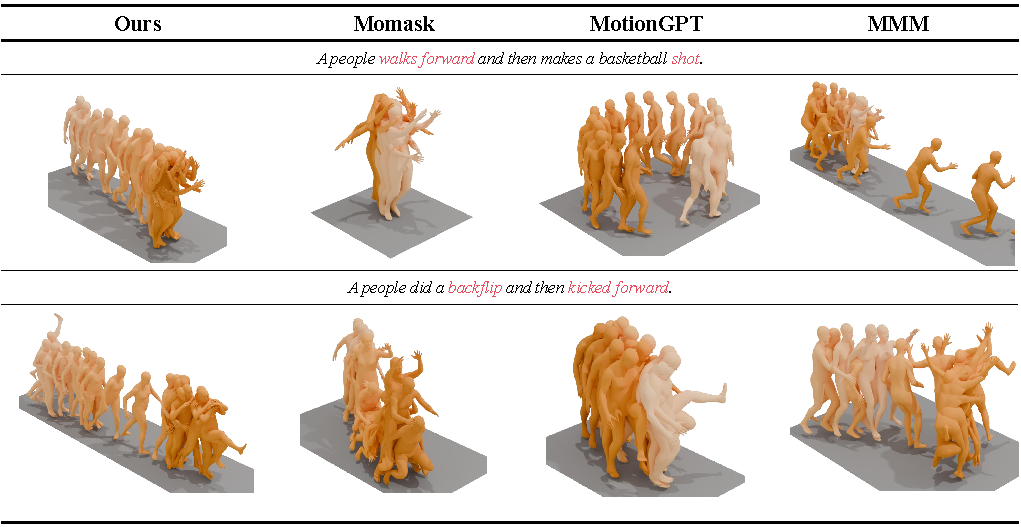
\includegraphics[width=1\linewidth]{fig_mogo/Ours_comparison_mogo_cropped.pdf}
    \caption{Qualitative comparison of generated motions produced by MOGO and other models. 
    Compared to prior methods Momask, MotionGPT, and MMM.
    }
    \label{fig:Qualitative experimental on text-to-motion.}
\end{figure*}
As shown in Fig.~\ref{fig:Qualitative experimental on text-to-motion.}, motions produced by our model are more semantically consistent with the input descriptions and exhibit smoother, more stable transitions without noticeable spatial drift. 


\subparagraph{Qualitative Results of Infinite Motion Generation}
\begin{figure*}[t] % 使用 figure 环境来处理图片
    \centering
    % 按照屏幕宽度自适应，高度保持比例填充
    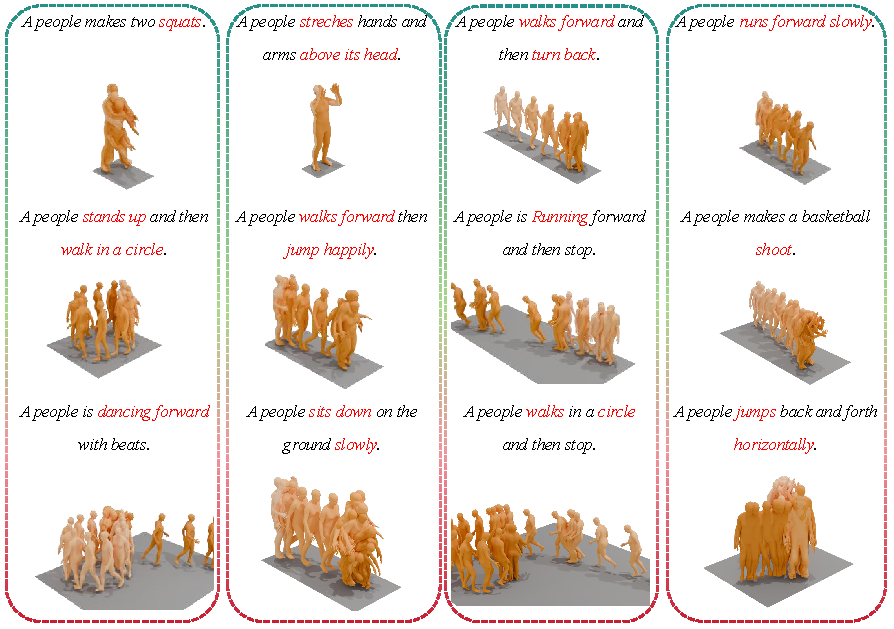
\includegraphics[width=1\textwidth]{fig_mogo/our_extend_motion_mogo_cropped.pdf}
    \caption{Motion Extension during Inference of MOGO.}
% 添加图片标题
    \label{fig:length}
\end{figure*}

Fig.~\ref{fig:length} showcases qualitative results of our infinite motion generation pipeline. Each vertical dashed box represents a complete generation sequence conditioned on a given text prompt. From top to bottom, the first row shows the initial motion segment, while the subsequent rows illustrate recursively generated motion continuations, conditioned on the same or semantically extended instruction.

Across all four examples, strong temporal consistency is demonstrated, with smooth transitions between motion segments and no noticeable discontinuities. The generated motions exhibit high semantic fidelity to the input descriptions, including complex behaviors such as “walks in a circle and then stop”, “jumps back and forth horizontally”, or “dancing forward with beats”, all of which are well executed over extended sequences. The smooth transition between action phrases (e.g., “stands up and then walk in a circle”) further indicates that both short-term dynamics and long-horizon dependencies are effectively captured.


% To support reproducibility and further inspection, we provide all visual examples shown in Figure~\ref{fig:length} as rendered videos, along with additional qualitative results in the supplementary materials. Specifically, the included \texttt{.zip} file contains not only video renderings corresponding to the figure, but also additional extended generations for diverse prompts—several of which feature single uninterrupted motion sequences exceeding 2000 frames in length. These results further demonstrate the stability of our model in synthesizing temporally consistent and semantically aligned motion over prolonged durations.

These results highlight the model’s capability to generate coherent, instruction-aligned motion indefinitely, making it suitable for real-world applications like virtual agents, gaming, and embodied language understanding.

\subparagraph{Qualitative Results of Single-Prompt Generation}
Fig.~\ref{fig:mogo_results} presents a comprehensive overview of our model's ability to generate motion sequences that align with a wide range of text prompts, demonstrating both semantic fidelity and fine-grained motion expressiveness. Each sample in the figure consists of a 3D motion mesh superimposed with motion trails (or motion blending) and its corresponding textual description, rendered in a stylized format where key action phrases are emphasized in red italics.

\begin{figure*}[htbp] % 使用 figure 环境来处理图片
    \centering
    % 按照屏幕宽度自适应，高度保持比例填充
    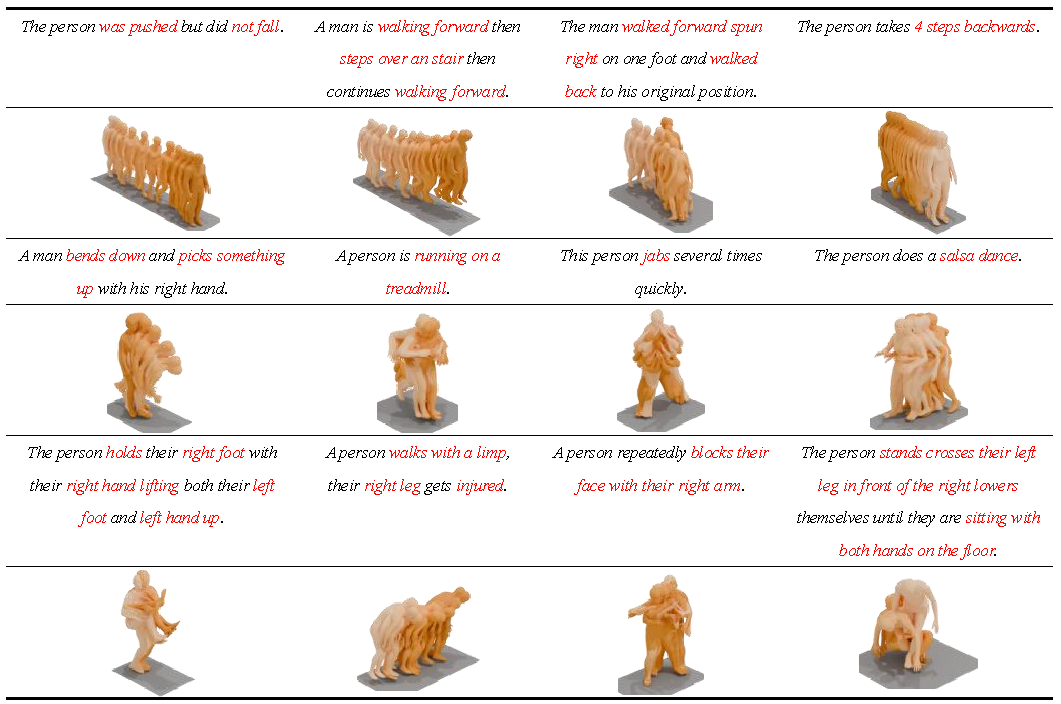
\includegraphics[width=1\textwidth]{fig_mogo/mogo_results_cropped.pdf}
    \caption{Genration Results of MOGO for single prompt} % 添加图片标题
    \label{fig:mogo_results} % 添加图片标签(不小心打成同名了)
\end{figure*}

Across the $4 \times 4$ grid layout, we showcase 16 distinct prompts covering a diverse set of actions, such as:
\begin{itemize}
    \item \textbf{Simple physical reactions:} \textit{``The person was pushed but did not fall.''}
    \item \textbf{Complex multi-phase motions:} \textit{``A man is walking forward then steps over a stair then continues walking forward.''}
    \item \textbf{Locomotion with intention shifts:} \textit{``walked forward spun right on one foot and walked back to his original position.''}
    \item \textbf{Fine-grained bodily behaviors:} \textit{``holds their right foot with their right hand lifting both their left foot and left hand up.''}
    \item \textbf{Stylized or culturally grounded motions:} \textit{``The person does a salsa dance.''}
    \item \textbf{Emotionally expressive behaviors:} \textit{``A person walks with a limp, their right leg gets injured.''}
\end{itemize}

These results indicate that our model is capable of capturing not only locomotion and spatial translation but also static poses, micro-movements, and non-trivial action transitions. The linguistic variations in the prompts are successfully translated into physically coherent movement, suggesting a high level of text-to-motion grounding.

\subsubsection{Ablation Studies}
\paragraph{Ablation Study on VAE Depth}
\begin{table}[t]
\centering
\scriptsize
\setlength{\tabcolsep}{10pt}
\renewcommand{\arraystretch}{1.2}
\begin{tabular}{cccc}
\toprule
\textbf{Depth} & \textbf{FID}$\downarrow$& \textbf{R TOP1 $\uparrow$} & MM-Dist$\downarrow$\\
\midrule
1 & 0.070$^{\pm 0.001}$ & 0.502 $^{\pm 0.001}$ & 2.999 $^{\pm 0.006}$\\
3 & 0.021$^{\pm 0.001}$  & 0.508 $^{\pm 0.001}$& 2.992 $^{\pm 0.008}$\\
6 & \textbf{0.016}$^{\pm 0.001}$ & 0.510 $^{\pm 0.001}$ & 2.989 $^{\pm 0.007}$\\
7 & 0.016$^{\pm 0.001}$ & 0.509 $^{\pm 0.001}$ & 2.996 $^{\pm 0.003}$\\
\bottomrule
\end{tabular}
\caption{The impact of different quantization layers on model reconstruction quality when the codebook size is $8192 \times 128$. Bold face indicates the best result.}
\label{tab:compare_vae_kitml}
\end{table}
The impact of quantization depth is evaluated by varying the number of layers while fixing the codebook size to $8192 \times 128$ (Table~\ref{tab:compare_vae_kitml}). A single-layer quantizer performs poorly (FID: 0.070), indicating limited capacity. Increasing to 3 layers significantly improves performance (FID: 0.021), and 6 layers yield the best overall results (FID: \textbf{0.016}, R-Top1: 0.510, MM-Dist: 2.989). Adding a 7th layer offers no further gain and slightly worsens MM-Dist, suggesting diminishing returns. Overall, 6-layer quantization provides the best balance between expressiveness and generalization.


\paragraph{Ablation Study on Layer-Head Configuration}
\begin{table}[t]
\centering
\scriptsize
\setlength{\tabcolsep}{6pt}
\renewcommand{\arraystretch}{1.5}

\begin{tabular}{ccccc}
\toprule
\textbf{Heads} & \textbf{Layers} & \textbf{FID}$\downarrow$ & \textbf{R-Top1}$\uparrow$ & \textbf{MM-Dist}$\downarrow$ \\
\midrule

\shortstack{[4, 4, 4,\\ 4, 4, 4]} & \shortstack{[6]} & 0.242$^{\pm 0.009}$ & 0.397$^{\pm 0.005}$ & 4.132$^{\pm 0.013}$ \\
\shortstack{[4, 4, 4,\\ 4, 4, 4]} & \shortstack{[6, 6, 6,\\ 6, 6, 6]} & 0.101$^{\pm 0.004}$ & 0.461$^{\pm 0.003}$ & 3.359$^{\pm 0.009}$ \\
\shortstack{[12, 6, 4,\\ 2, 2, 2]} & \shortstack{[16, 8, 6,\\ 4, 2, 2]} & 0.077$^{\pm 0.003}$ & 0.473$^{\pm 0.003}$ & 3.260$^{\pm 0.010}$ \\
\shortstack{[16, 8, 4,\\ 2, 2, 2]} & \shortstack{[18, 10, 6,\\ 4, 2, 2]} & 0.058$^{\pm 0.003}$ & 0.490$^{\pm 0.002}$ & 3.168$^{\pm 0.009}$ \\
\shortstack{[16, 12, 4,\\ 2, 2, 2]} & \shortstack{[18, 16, 6,\\ 4, 2, 2]} & 0.044$^{\pm 0.004}$ & 0.508$^{\pm 0.003}$ & 3.063$^{\pm 0.010}$ \\
\shortstack{[16, 12, 6,\\ 2, 2, 2]} & \shortstack{[18, 16, 8,\\ 4, 2, 2]} & \textbf{0.038}$^{\pm 0.002}$ & \textbf{0.515}$^{\pm 0.003}$ & \textbf{2.951}$^{\pm 0.008}$ \\
\bottomrule
\end{tabular}
\caption{
Impact of model depths and head configurations on HumanML3D results (codebook size: $8192 \times 128$). Bold indicates the best performance.
}
\label{tab:compare_RQHC_kitml}
\end{table}

The impact of Transformer depth and attention head configurations on HumanML3D is studied (Table~\ref{tab:compare_RQHC_kitml}). Starting from a uniform setup (\texttt{[4, 4, 4, 4, 4, 4]} layers, \texttt{[6, 6, 6, 6, 6, 6]} heads), the model yields suboptimal results (FID 0.101, MM-Dist 3.359). With deeper, hierarchically structured layers and progressively narrower heads, performance improves consistently. The best configuration (\texttt{[18, 16, 8, 4, 2, 2]} layers, \texttt{[16, 12, 6, 2, 2, 2]} heads) achieves the lowest FID (\textbf{0.079}), highest R-Top1 (\textbf{0.505}), and lowest MM-Dist (\textbf{3.002}).

These findings suggest that allocating more depth in early stages and gradually reducing head width enables better modeling of both global semantics and local temporal details. Compared to uniformly scaled variants, hierarchical designs yield stronger R-Top1 and MM-Dist, highlighting the importance of architectural balance.


\paragraph{Qualitative Examples for Ablation Study on TCA}
\subparagraph{Example 1. (Humanml3D Test)}
\begin{itemize}
  \item \textbf{Raw prompt:}  
        \emph{``Someone imitating a golf swing.''}
  \item \textbf{Normalized:}  
        \emph{``Raise arms, swing forward, return to stance.''}
  \item \textbf{Thinking process:}
  
         1. Lift both arms as if holding a golf club \\
         2. Swing the arms forward in an arc \\
         3. Return to a relaxed standing posture \\
  \item \textbf{Final rewritten instruction:}\\
        \emph{``A person lifts both arms, swings them forward in an arc, and returns to a standing position.''}
\end{itemize}

\subparagraph{Example 2. (Wild data Test)}
\begin{itemize}
  \item \textbf{Raw prompt:}  
        \emph{``A human is practicing expressive spinning gestures.''}
  \item \textbf{Normalized:}  
        \emph{``Spin, pause, raise arms.''}
  \item \textbf{Steps:}

1. Spin once on the spot \\
2. Hold still for a beat \\
3. Raise both hands \\

  \item \textbf{Final rewritten instruction:}\\
        \emph{``A person spins once on the spot, holds still briefly, and raises both hands.''}
\end{itemize}

\subparagraph{Example 3. (Wild data Test)}
\begin{itemize}
  \item \textbf{Raw prompt:}  
        \emph{``A human is rehearsing a dynamic forward motion sequence.''}
  \item \textbf{Normalized:}  
        \emph{``Walk, crouch, roll forward, stand.''}
  \item \textbf{Steps:}
  
1. Walk forward \\
2. Drop into a crouch\\
3. Roll forward\\
4. Stand upright\\

  \item \textbf{Final rewritten instruction:}\\
        \emph{``A person walks forward, drops into a crouch, rolls ahead, and stands upright.''}
\end{itemize}


\begin{figure*}[t] % 使用 figure 环境来处理图片
    \centering
    % 按照屏幕宽度自适应，高度保持比例填充
    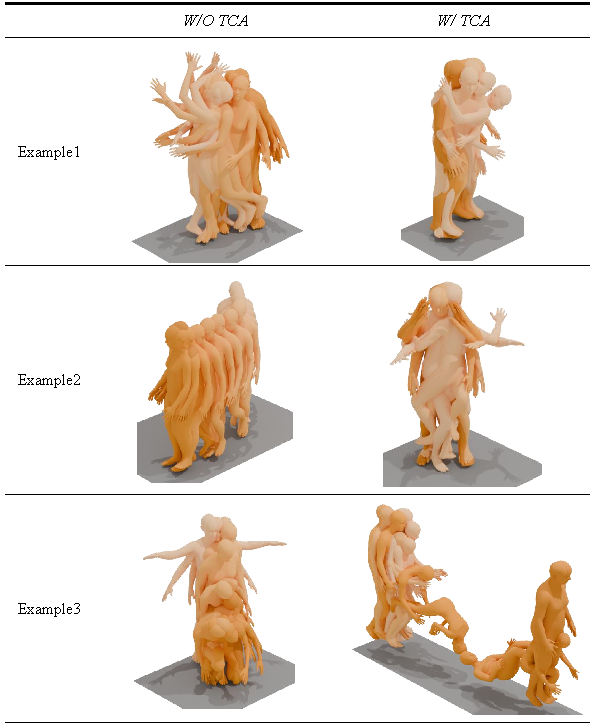
\includegraphics[width=0.65\textwidth]{fig_mogo/tca.pdf}
    \caption{
Comparison of motion sequences generated with and without Text Condition Alignment (TCA). 
TCA improves temporal coherence and semantic clarity, yielding more realistic and faithful motions.
}
    \label{fig:tca_compare}
\end{figure*}


As shown in Fig.~\ref{fig:tca_compare}, these cases show how TCA strategy reliably converts noisy,
multi-clause requests into concise, executable motion scripts—enabling the
decoder to render complex behaviours with accurate temporal structure \emph{without
any motion-model fine-tuning}.

\paragraph{Impact of Learnable Scaling in MoSA-VQ}
The role of the proposed learnable scaling mechanism in MoSA-VQ is investigated by comparing models with and without this design. In the baseline configuration, residual features at each quantization level are directly quantized without any adaptive normalization. In contrast, the full model applies a layer-specific affine transformation before quantization, allowing each level to adjust the residual space dynamically. As shown in Table~\ref{tab:ablation_scaled_weight}, incorporating learnable scale and bias parameters leads to consistent improvements across multiple evaluation metrics. Improved reconstruction quality, enhanced alignment between motion and text, and stronger semantic consistency are achieved. These results highlight the benefit of introducing adaptive normalization in residual quantization, which facilitates more expressive and stable token representations.


\begin{table}[t]
  \centering
  \scriptsize
  \renewcommand{\arraystretch}{1}
  \begin{minipage}[t]{0.48\linewidth}
    \centering
    \textbf{w/ Learnable Scaling} \\
    \begin{tabular}{c|ccc}
      \toprule
      \textbf{Codebook} & FID$\downarrow$ & R-Top1$\uparrow$ & MM-Dist$\downarrow$ \\
      \midrule
      2048$\times$512 & 0.052$\pm$0.005 & 0.498$\pm$0.002 & 2.997$\pm$0.008 \\
      4096$\times$256 & 0.047$\pm$0.005 & 0.501$\pm$0.002 & 2.901$\pm$0.008 \\
      8192$\times$128 & \textbf{0.038}$\pm$0.003 & \textbf{0.515}$\pm$0.007 & 2.951$\pm$0.003 \\
      \bottomrule
    \end{tabular}
  \end{minipage}
  \hfill
  \begin{minipage}[t]{0.48\linewidth}
    \centering
    \textbf{w/o Learnable Scaling} \\
    \begin{tabular}{c|ccc}
      \toprule
      \textbf{Codebook} & FID$\downarrow$ & R-Top1$\uparrow$ & MM-Dist$\downarrow$ \\
      \midrule
      2048$\times$512 & 0.094$\pm$0.011 & 0.484$\pm$0.002 & 3.273$\pm$0.009 \\
      4096$\times$256 & 0.091$\pm$0.004 & 0.493$\pm$0.004 & 3.451$\pm$0.017 \\
      8192$\times$128 & \textbf{0.079}$\pm$0.002 & \textbf{0.502}$\pm$0.002 & 3.002$\pm$0.008 \\
      \bottomrule
    \end{tabular}
  \end{minipage}
  \caption{Ablation study on the use of learnable scaling. We evaluate various codebook sizes on HumanML3D.}
      \label{tab:ablation_scaled_weight}
\end{table}

\paragraph{Impact of prompt and quantization}
\begin{figure*}[t] % 使用 figure 环境来处理图片
    \centering
    % 按照屏幕宽度自适应，高度保持比例填充
    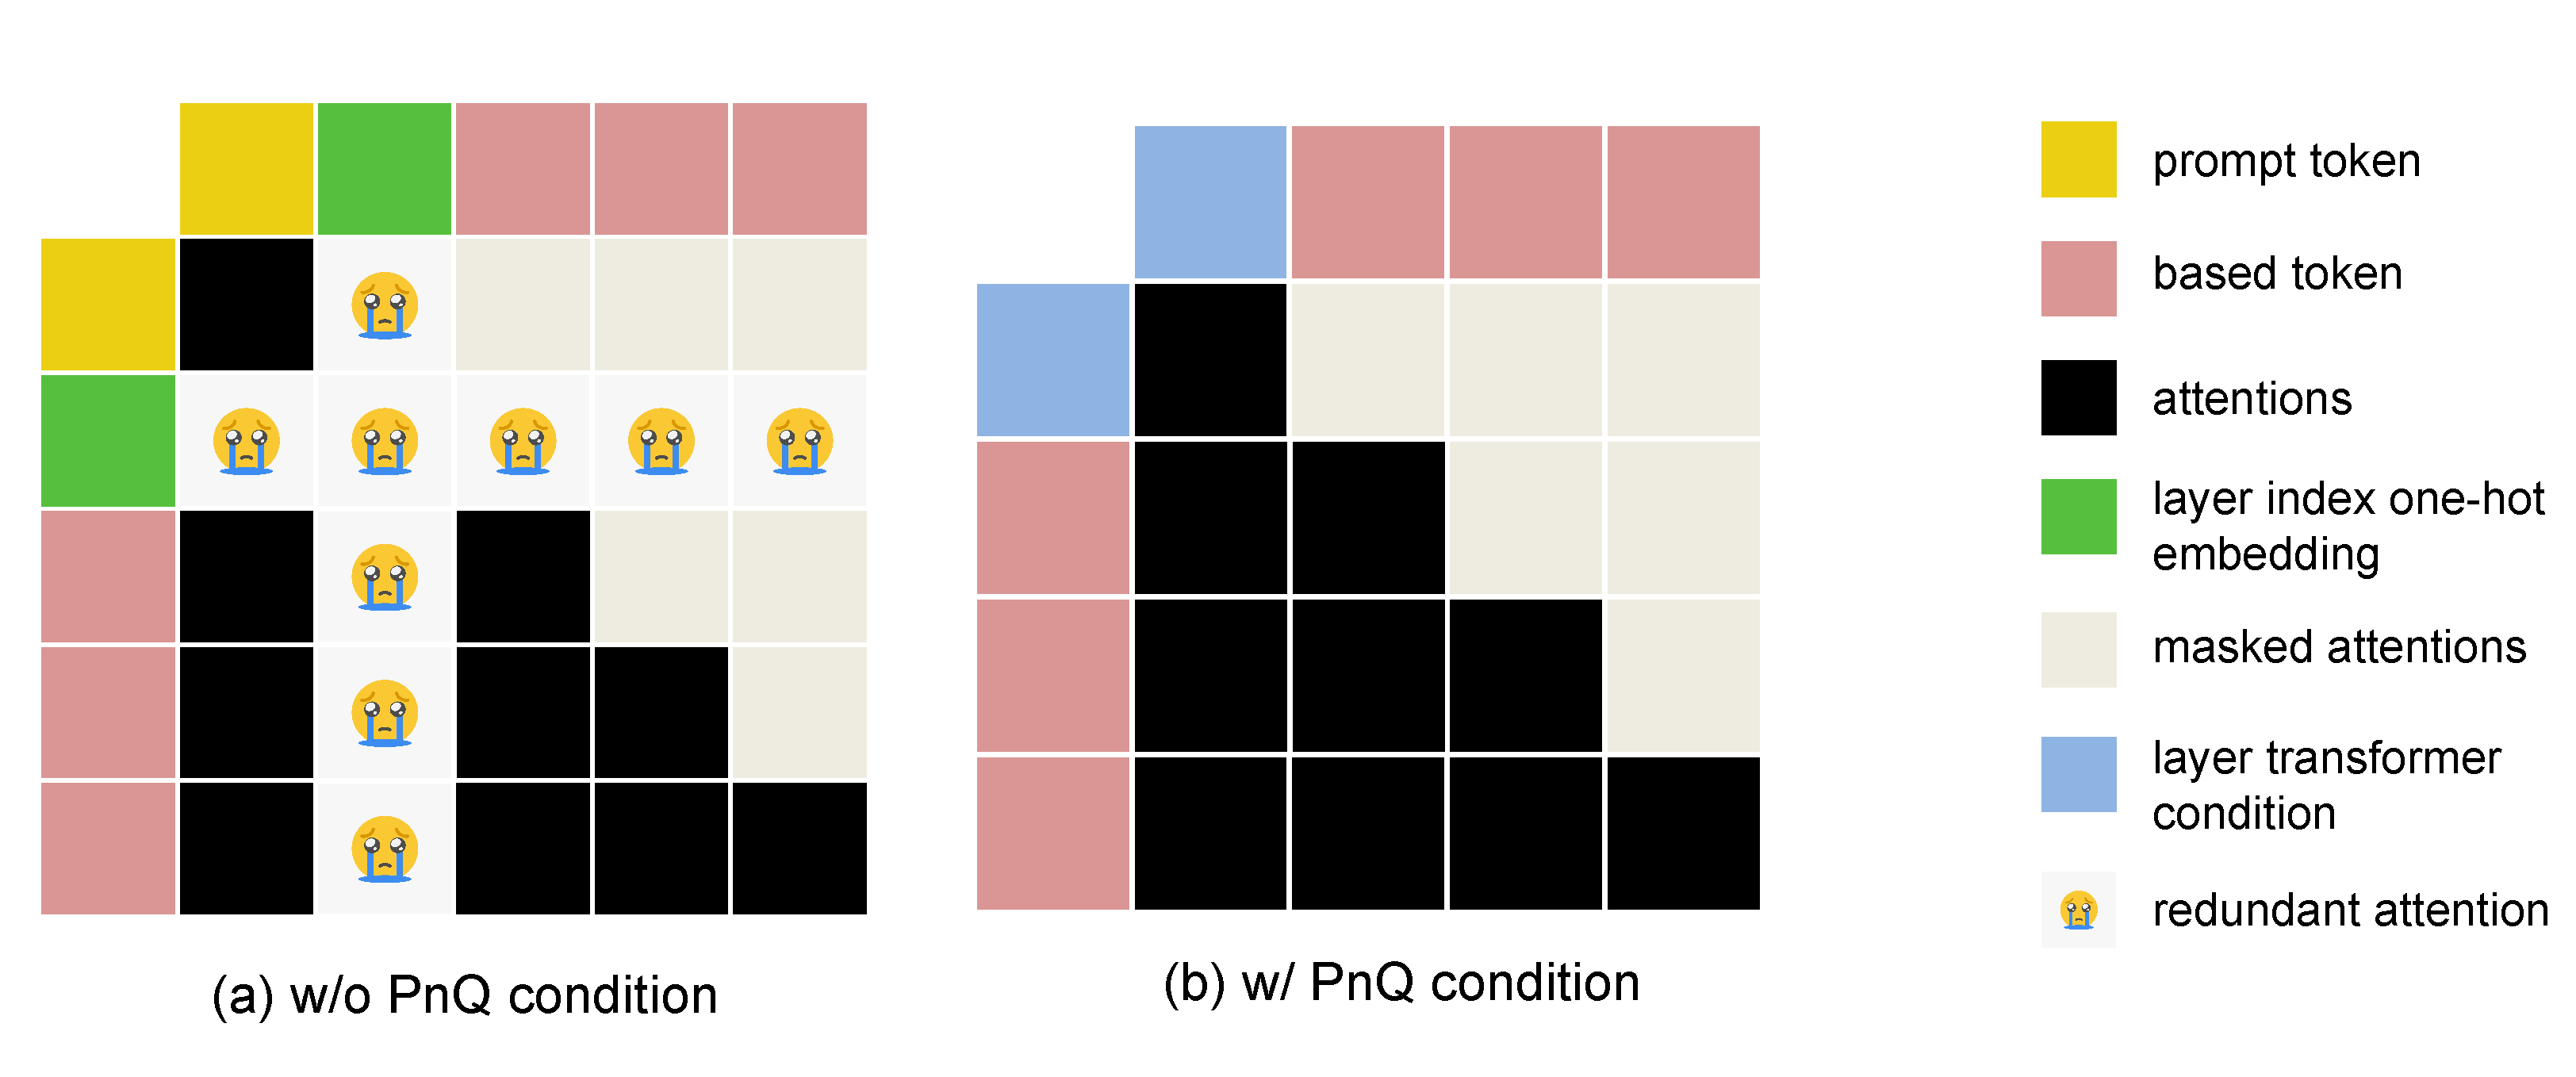
\includegraphics[width=1\textwidth]{fig_mogo/Mogo_Attention.pdf}
    \caption{Comparison of attention patterns with and without the PnQ (Prompt and Quantization) condition}
% 添加图片标题
    \label{fig:architechure2} % 添加图片标签(不小心打成同名了)
\end{figure*}

\subparagraph{Without PnQ} An additional layer token is inserted between the textual prompt and the quantized motion sequence, serving as an intermediate fusion node. However, this design introduces a level of indirection that leads to redundant attention computation and diluted gradient flow. As a result, the model exhibits weaker cross-modal alignment, as the semantic linkage between text and motion must be learned indirectly through this intermediate token, which may act as a bottleneck in representation transfer.

\subparagraph{With PnQ} 
As shown in Fig.~\ref{fig:architechure2}, the prompt token is fused directly with the quantization condition tokens through positional and conditional injection. This eliminates the need for an intermediate token and allows a more direct and semantically grounded connection to be established between the text prompt and motion representation. Consequently, this design not only improves attention efficiency—by reducing unnecessary detours in the attention graph—but also enhances cross-modal alignment by preserving semantic consistency throughout the sequence.


\paragraph{Effect of Dataset Size}
\begin{table}[t]
  \centering
  \scriptsize

  \label{tab:combined_fid_realtime}
  \renewcommand{\arraystretch}{1.15}

  \begin{minipage}[t]{0.48\linewidth}
    \centering
    \textbf{(a) Dataset Size vs. FID} \\
    \vspace{0.3em}
    \begin{tabular}{c|ccc}
      \toprule
      \textbf{Epochs} & \textbf{0\% CMP} & \textbf{50\% CMP} & \textbf{100\% CMP} \\
      \midrule
      50  & 0.671  & 0.601  & 0.501  \\
      80  & 0.437  & 0.379  & 0.284  \\
      100 & 0.347  & 0.263  & \textbf{0.205} \\
      \bottomrule
    \end{tabular}
  \end{minipage}
  \hfill
  \begin{minipage}[t]{0.48\linewidth}
    \centering
    \textbf{(b) Real-time Inference (A800)} \\
    \vspace{0.3em}
    \begin{tabular}{lccc}
      \toprule
      \textbf{Method}  & \textbf{AITS${\uparrow}$} & \textbf{Params} & \textbf{FID${\downarrow}$} \\
      \midrule
      MLD          & 0.14 & 34M & 0.473          \\
      MotionGPT    & 0.81 & 770M & 0.160          \\
      MoMask       & \textbf{0.06} & 163M & 0.045   \\
      MOGO         & 0.37 & 830M & \textbf{0.038} \\
      \bottomrule
    \end{tabular}
  \end{minipage}
      \caption{Left: Effect of dataset size on FID. Right: Real-time inference comparison on A800.}
  \label{tab:dataset_size_fid}

\end{table}

To investigate the scalability of MOGO, performance is evaluated under different training set sizes by progressively mixing HumanML3D with 50\% and 100\% proportions of the CMP dataset. Crucially, the MoSA-VQ quantizer is kept frozen during this process to isolate the impact of data volume on downstream generation quality.

As shown in Table~\ref{tab:dataset_size_fid}(a), increasing the amount of training data leads to consistent improvements in FID across training epochs. For instance, at 100 training epochs, FID drops from 0.347 (with only HumanML3D) to 0.263 with 50\% CMP, and further to 0.205 with full CMP integration. This trend holds across earlier epochs as well, demonstrating that larger and more diverse motion data helps the model generalize better, even without modifying the discrete representation space.

These results highlight the scalability and data efficiency of MOGO’s architecture, as well as the robustness of the MoSA-VQ quantizer in accommodating novel distributions through fixed codes.


\paragraph{Effect of Codebook Size}

\begin{table*}[t]

  \centering
  \small
  \setlength{\tabcolsep}{7pt} % 默认是6pt，略微拉开
  \renewcommand{\arraystretch}{1.2} % 拉开行距

  \resizebox{0.9\textwidth}{!}{
    \begin{tabular}{c c c c | c c c}
      \toprule
      \multirow{2}{*}{\textbf{Codebook Size}} & \multicolumn{3}{c|}{\textbf{Reconstruction}} & \multicolumn{3}{c}{\textbf{Generation}} \\
      \cmidrule(lr){2-7}
      & \textbf{FID$\downarrow$} & \textbf{Top1$\uparrow$} & \textbf{MM-Dist$\downarrow$}
      & \textbf{FID$\downarrow$} & \textbf{Top1$\uparrow$} & \textbf{MM-Dist$\downarrow$} \\
      \midrule
      512 $\times$ 512     & 0.022$\pm$0.001 & 0.508$\pm$0.003 & 2.997$\pm$0.007 & 0.203$\pm$0.009 & 0.469$\pm$0.002 & 3.138$\pm$0.006 \\
      1024 $\times$ 1024   & {0.015}$\pm$0.001 & 0.511$\pm$0.002 & 2.984$\pm$0.010 & 0.114$\pm$0.008 & 0.467$\pm$0.003 & 3.114$\pm$0.009 \\
      2048 $\times$ 512    & 0.017$\pm$0.001 & 0.511$\pm$0.003 & 2.980$\pm$0.007 & 0.052$\pm$0.005 & 0.498$\pm$0.002 & 2.997$\pm$0.008 \\
      4096 $\times$ 256    & 0.019$\pm$0.001 & 0.510$\pm$0.002 & 2.989$\pm$0.006 & 0.047$\pm$0.005 & 0.501$\pm$0.002 & 2.901$\pm$0.008 \\
      8192 $\times$ 128    & \textbf{0.013}$\pm$0.001 & 0.510$\pm$0.002 & 2.989$\pm$0.007 & \textbf{0.038}$\pm$0.003 & 0.515$\pm$0.007 & 2.951$\pm$0.003 \\
      \bottomrule
    \end{tabular}
  }
    \caption{Study on the number of codes in codebook on HumanML3D~\cite{guo2022generating} test set. \textbf{Bold} indicates the best FID result.}
  \label{ablation:codebooksize}
\end{table*}

An ablation study is conducted to investigate how different codebook sizes affect both reconstruction and generation quality. Specifically, the number of entries and dimensions in the codebook is varied, and performance is evaluated on the HumanML3D test set in terms of FID, Top-1 Accuracy, and MM-Distance. Results are summarized in Table~\ref{ablation:codebooksize}.

As shown in the table, larger codebooks generally lead to better performance, particularly in the generation setting. When the codebook size is increased from $512 \times 512$ to $8192 \times 128$, the generation FID steadily decreases from 0.203 to 0.038, indicating a substantial improvement in motion realism. Similarly, Top-1 Accuracy improves from 0.469 to 0.515, and MM-Distance also decreases, suggesting enhanced semantic alignment and diversity.

In the reconstruction setting, a similar trend is observed: the FID drops from 0.022 to 0.013 as the codebook size increases. Notably, while some intermediate configurations (e.g., $1024 \times 1024$) achieve marginally better reconstruction FID (0.015), they underperform in generation quality, highlighting that optimal reconstruction does not always translate to optimal generation.

The best overall performance is achieved with a codebook size of $8192 \times 128$, which provides a favorable balance between code granularity and diversity. This configuration yields the lowest FID in both reconstruction and generation settings, while maintaining competitive Top-1 Accuracy and MM-Distance. These results demonstrate that increasing the expressiveness of the codebook—by enlarging its capacity—enables the quantizer to better capture fine-grained motion semantics and contributes to improved generative performance downstream.


\paragraph{Effect of Cross-Level Decorrelation Loss}
\begin{table}[t]
\centering
\footnotesize
\setlength{\tabcolsep}{10pt}
\renewcommand{\arraystretch}{1.2}

\begin{tabular}{cccc}
\toprule
\textbf{decorrelation loss} & \textbf{FID}$\downarrow$& \textbf{R TOP1 $\uparrow$} & MM-Dist$\downarrow$\\
\midrule
w/o & 0.044$^{\pm 0.001}$ & 0.503 $^{\pm 0.001}$ & 2.996 $^{\pm 0.006}$\\
w/ & 0.038$^{\pm 0.001}$  & 0.508 $^{\pm 0.001}$& 2.992 $^{\pm 0.008}$\\
\bottomrule
\end{tabular}
\caption{Decorrelation loss evaluation on HumanML3D}
\label{tab:compare_vae_kitml}
\end{table}
To validate the effectiveness of the proposed cross-level decorrelation loss, an ablation experiment is conducted on the HumanML3D test set, as shown in Table~\ref{tab:compare_vae_kitml}. Two settings are compared: one using the full training objective (including $\mathcal{L}_{\text{decor}}$), and one without it.

When the decorrelation loss is removed, a slight degradation in generation quality is observed, with FID increasing from 0.038 to 0.044. Moreover, R-Top1 accuracy drops from 0.508 to 0.503, and MM-Distance increases from 2.992 to 2.996, indicating reduced semantic alignment and less precise generation.

This performance gap, although modest in absolute value, is consistent across all metrics and can be attributed to inter-level redundancy present when $\mathcal{L}_{\text{decor}}$ is absent. As defined in Eq.~(\ref{eq:decoLa}), the decorrelation loss minimizes the batch-wise covariance between the quantized vector $\boldsymbol{\phi}^l$ and the residual $\mathbf{r}^{l+1}$ at the next level. This enforces statistical orthogonality across quantization layers, effectively disentangling the hierarchical representations.

From an information-theoretic standpoint, this encourages each level to capture novel, non-overlapping features, which reduces redundancy and improves latent code efficiency. In practice, this regularization leads to more compact and expressive codes—especially important under constrained codebook budgets or when deeper quantization hierarchies are used.

In summary, the proposed cross-level decorrelation loss plays a crucial role in enhancing both the semantic clarity and compression efficiency of the quantization framework, and leads to measurable improvements in motion generation quality.

% =========================================================
% 5. Discussion
% =========================================================
% \section{Discussion}

% \subsection{Challenges and Observations}
% Our experiments demonstrate that both MotionDirector and MOGO advance the state of the art in complementary aspects of motion generation. However, several challenges remain. 

% For MotionDirector, while the integration of video priors and dual conditioning substantially improves spatio-temporal fidelity and semantic grounding, we observed sensitivity to the quality of video inputs. Noisy or low-quality videos sometimes led to unstable representations despite the use of DUET and the Dynamic Mask Mechanism. In addition, the auto-guidance mechanism, although effective in balancing modalities without manual weight tuning, occasionally introduced over-corrections when the text and video conditions were weakly aligned. This suggests that further work is needed to improve robustness under noisy multimodal conditions, particularly for open-domain prompts.

% For MOGO, the autoregressive formulation successfully enables infinite-length generation with high temporal coherence. The hierarchical quantization and causal decoding design alleviated token interference and error accumulation observed in previous tokenization-based approaches. Nonetheless, autoregressive decoding inherently introduces computational overhead for very long sequences. Although our design supports one-pass inference and relative positional encoding, the runtime cost still scales linearly with sequence length. Another limitation lies in the representation capacity of MoSA-VQ: while adaptive scaling and cross-level decorrelation improved efficiency, extremely complex or high-frequency motions remain challenging to encode compactly.

% \subsection{Comparison with Existing Methods}
% Compared to diffusion-based text-to-motion approaches (e.g., MDM, MotionDiffuse, MLD), MotionDirector provides stronger multimodal controllability by directly leveraging video priors. This results in improved structural fidelity and richer expressiveness, while retaining compatibility with textual editing. By contrast, MOGO offers a distinct advantage over both diffusion and prior VQ–transformer approaches: it achieves infinite-length, prompt-adaptive generation, which is particularly valuable for real-time or interactive applications. Taken together, these frameworks extend the capabilities of motion generation beyond short, single-task pipelines.

% \subsection{Limitations and Future Directions}
% While our methods substantially improve flexibility and control in motion generation, several limitations highlight promising avenues for future research. 

% For \textbf{MotionDirector}, the current framework primarily relies on rendered video data derived from HumanML3D, which, although useful for benchmarking, lacks the richness and variability of real-world video. This discrepancy limits the realism and generalization of the generated motions. A key direction is therefore to design more effective training paradigms that tightly integrate real-world video data into the motion generation pipeline. By combining textual prompts, video trajectories, and other multimodal cues in a unified conditioning space, we aim to achieve motion synthesis that is both more faithful to natural human behaviors and more controllable within 3D environments.

% For \textbf{MOGO}, although the hierarchical autoregressive design enables infinite-length generation, its current form does not yet fully address model efficiency and interpretability. Lightweight decoding strategies are necessary to make long-horizon autoregression computationally viable in practice. Moreover, the motion quantization module (MoSA-VQ) could be further refined to provide more task-specific representations that align with the semantics and dynamics of motion generation. Improving the interpretability of motion codes would not only facilitate more transparent analysis of model behavior but also open the door to higher-level editing and controllability in downstream applications.

% Overall, bridging MotionDirector’s multimodal conditioning with real-world data and enhancing MOGO’s hierarchical representation with greater efficiency and interpretability represent two complementary and essential directions toward building the next generation of realistic, controllable, and scalable motion generation frameworks.

\section{Discussion}

\subsection{Challenges and Observations}
The experiments demonstrate that both MotionDirector and MOGO advance the state of the art in complementary aspects of motion generation. However, several challenges remain. 

For MotionDirector, while the integration of video priors and dual conditioning substantially improves spatio-temporal fidelity and semantic grounding, sensitivity to the quality of video inputs is observed. Noisy or low-quality videos sometimes lead to unstable representations despite the use of DUET and the Dynamic Mask Mechanism. In addition, the auto-guidance mechanism, although effective in balancing modalities without manual weight tuning, occasionally introduces over-corrections when the text and video conditions are weakly aligned. This suggests that further work is needed to improve robustness under noisy multimodal conditions, particularly for open-domain prompts.

For MOGO, the autoregressive formulation successfully enables infinite-length generation with high temporal coherence. The hierarchical quantization and causal decoding design alleviates token interference and error accumulation observed in previous tokenization-based approaches. Nonetheless, autoregressive decoding inherently introduces computational overhead for very long sequences. Another limitation lies in the representation capacity of MoSA-VQ: while adaptive scaling and cross-level decorrelation improve efficiency, extremely complex or high-frequency motions remain challenging to encode compactly.

\subsection{Comparison with Existing Methods}
Compared to diffusion-based text-to-motion approaches (e.g., MDM, MotionDiffuse, MLD), MotionDirector provides stronger multimodal controllability by directly leveraging video priors. This results in improved structural fidelity and richer expressiveness, while retaining compatibility with textual editing. By contrast, MOGO offers a distinct advantage over both diffusion and prior VQ–transformer approaches: it achieves infinite-length, prompt-adaptive generation, which is particularly valuable for real-time or interactive applications. Taken together, these frameworks extend the capabilities of motion generation beyond short, single-task pipelines.

\subsection{Limitations and Future Directions}
While the proposed methods substantially improve flexibility and control in motion generation, several limitations highlight promising avenues for future research. 

For \textbf{MotionDirector}, the current framework primarily relies on rendered video data derived from HumanML3D, which, although useful for benchmarking, lacks the richness and variability of real-world video. This discrepancy limits the realism and generalization of the generated motions. A key direction is therefore to design more effective training paradigms that tightly integrate real-world video data into the motion generation pipeline. By combining textual prompts, video trajectories, and other multimodal cues in a unified conditioning space, motion synthesis that is both more faithful to natural human behaviors and more controllable within 3D environments may be achieved.

For \textbf{MOGO}, although the hierarchical autoregressive design enables infinite-length generation, its current form does not yet fully address model efficiency and interpretability. Lightweight decoding strategies are necessary to make long-horizon autoregression computationally viable in practice. Moreover, the motion quantization module (MoSA-VQ) could be further refined to provide more task-specific representations that align with the semantics and dynamics of motion generation. Improving the interpretability of motion codes would not only facilitate more transparent analysis of model behavior but also open the door to higher-level editing and controllability in downstream applications.

Overall, bridging MotionDirector’s multimodal conditioning with real-world data and enhancing MOGO’s hierarchical representation with greater efficiency and interpretability represent two complementary and essential directions toward building the next generation of realistic, controllable, and scalable motion generation frameworks.




% TODO：数据偏差、物理合理性、开源/部署与伦理边界。

% =========================================================
% 6. Future Work  —— replaced by NEW PLAN
% =========================================================

\section{Future Work}
\label{sec:future}

Looking ahead, the next stage of this research will focus on consolidating the advances made so far into a unified system for controllable and scalable human motion generation. Two key research goals will guide the work: (\textit{i}) exploring the complementary advantages of autoregressive and diffusion-based paradigms for motion generation, and (\textit{ii}) enhancing controllability to achieve precise manipulation of motions in 3D space.

First, while autoregressive models such as MOGO excel at streamable, infinite-length generation with strong temporal consistency, diffusion models like MotionDirector demonstrate superior sample diversity and robust multimodal conditioning. A natural next step is to integrate these two paradigms, combining tokenized motion representations with multimodal diffusion to enable faster, more expressive, and more controllable sampling. Such hybrid designs may also alleviate the computational overhead of long-horizon autoregression while preserving its coherence benefits.

Second, beyond high-level guidance from text or video, future work will expand the control axes toward fine-grained, spatially explicit constraints. This includes trajectory-level specification, contact events with the environment, stylistic variations, and clothing or soft-body dynamics. By enabling users to specify not only what motion to generate but also where and how it unfolds in 3D space, the system will progress from approximate semantic alignment to precise spatial control.

In summary, the future research agenda will pursue: 
\begin{itemize}
    \item Integrating autoregressive and diffusion-based approaches for faster and more controllable sampling,
    \item Expanding controllable dimensions to include trajectory, contact, style, and clothing dynamics,
    \item Enhancing generalization with scalable pretraining strategies and improving robustness under diverse real-world inputs.
\end{itemize}

These directions will further advance the long-term objective of this project: to build practical, interactive systems for avatars, AR/VR, and robotics, where precision, controllability, stability, and efficiency must be achieved simultaneously.


% \section{Future Work}
% Looking forward, the next phase will focus on consolidating these advances into a unified system. Key directions include: (i) combining tokenized motion representations with multimodal diffusion for faster and more controllable sampling, (ii) expanding control axes to encompass trajectory, contact, style, and apparel dynamics, and (iii) strengthening generalization to in-the-wild data through scalable pretraining and robust alignment strategies. These directions will further advance the project’s long-term goal of building practical interactive systems for avatars, AR/VR, and robotics, where precision, controllability, and efficiency must be achieved together.


% \subsection{Motion-Style Transformation via Flow Matching with Video Conditioning}
% We will frame motion-style transformation as a conditional generation problem, closely following the setup popularized by Boeun~Kim for motion style transfer. Short reference \emph{video clips} will serve as the conditioning signal.

% \paragraph{Core idea.}
% We plan to adapt \emph{Flow Matching} (FM)—a faster, single-step alternative to classical diffusion that also underpins Stable Diffusion~3—to motion-style transfer. Given a short reference video, the model starts from a simple Gaussian latent and transports it to a \emph{video latent} that matches the source content while adopting the reference motion style. Since the reference clip already carries rich temporal cues, the source and target distributions are near each other; we expect faster training and fewer inference steps than typical image FM or DDPM pipelines.


% \paragraph{Architecture and conditioning.}
% A conditional fusion module will integrate the video prior with text/motion inputs, reusing our MotionDirector-style fusion choices (e.g., add/concat/hadamard and cross-/self-attention variants). The target trajectory in latent space will be learned with FM losses; we will experiment with different noise scales and velocity parameterizations.

% \subsection{Hybrid Autoregressive + Diffusion Video Architecture with a 3D Causal VAE}
% We also plan to investigate a trending video architecture that combines \emph{autoregressive} (AR) models with \emph{diffusion}, typically built on top of a 3D \emph{causal VAE} that factorizes spatial and temporal paths while learning a shared video representation.

% \paragraph{Motivation.}
% AR excels at real-time, streaming generation and low-latency continuation; diffusion provides fine-grained, step-wise refinement and stronger perceptual quality. A hybrid system can leverage AR for fast drafts and diffusion as a corrector.

% \paragraph{Tokenizer and representation.}
% We will train or reuse a 3D causal VAE that produces spatiotemporal latents (e.g., token grids) suitable for both AR decoding and diffusion refinement. The tokenizer should scale cleanly from single images to longer videos, enabling unified handling of keyframes and full sequences.

% \paragraph{Hybrid generator.}
% The AR branch will autoregressively stream tokens conditioned on text/motion inputs (and optional video priors). A lightweight diffusion branch will operate as a corrector/refiner (e.g., on residuals or a lower-rate schedule), improving fidelity and temporal coherence with minimal extra latency.

% \paragraph{Training strategy.}
% We will explore staged training: (1) pretrain the VAE tokenizer, (2) train the AR generator for stable streaming, and (3) add diffusion refinement with teacher-forced or replay buffers. Joint end-to-end finetuning will be evaluated for stability and quality.

% \paragraph{Evaluation and real-time targets.}
% We will measure frame latency, throughput, long-horizon consistency, retrieval precision, and distributional distances. Streaming demos will test prompt switching, looping, and content injections.

% \paragraph{Ablations and risks.}
% We will ablate AR context length, diffusion step counts, tokenizer rates, and causal masking strategies. Risks include compounding AR drift and cost of diffusion passes; mitigations include scheduled corrector calls, reset anchors, and online constraints.

\subsection{Timeline and Milestones}
\label{sec:timeline}
\begin{figure*}[tbp]
    \centering
    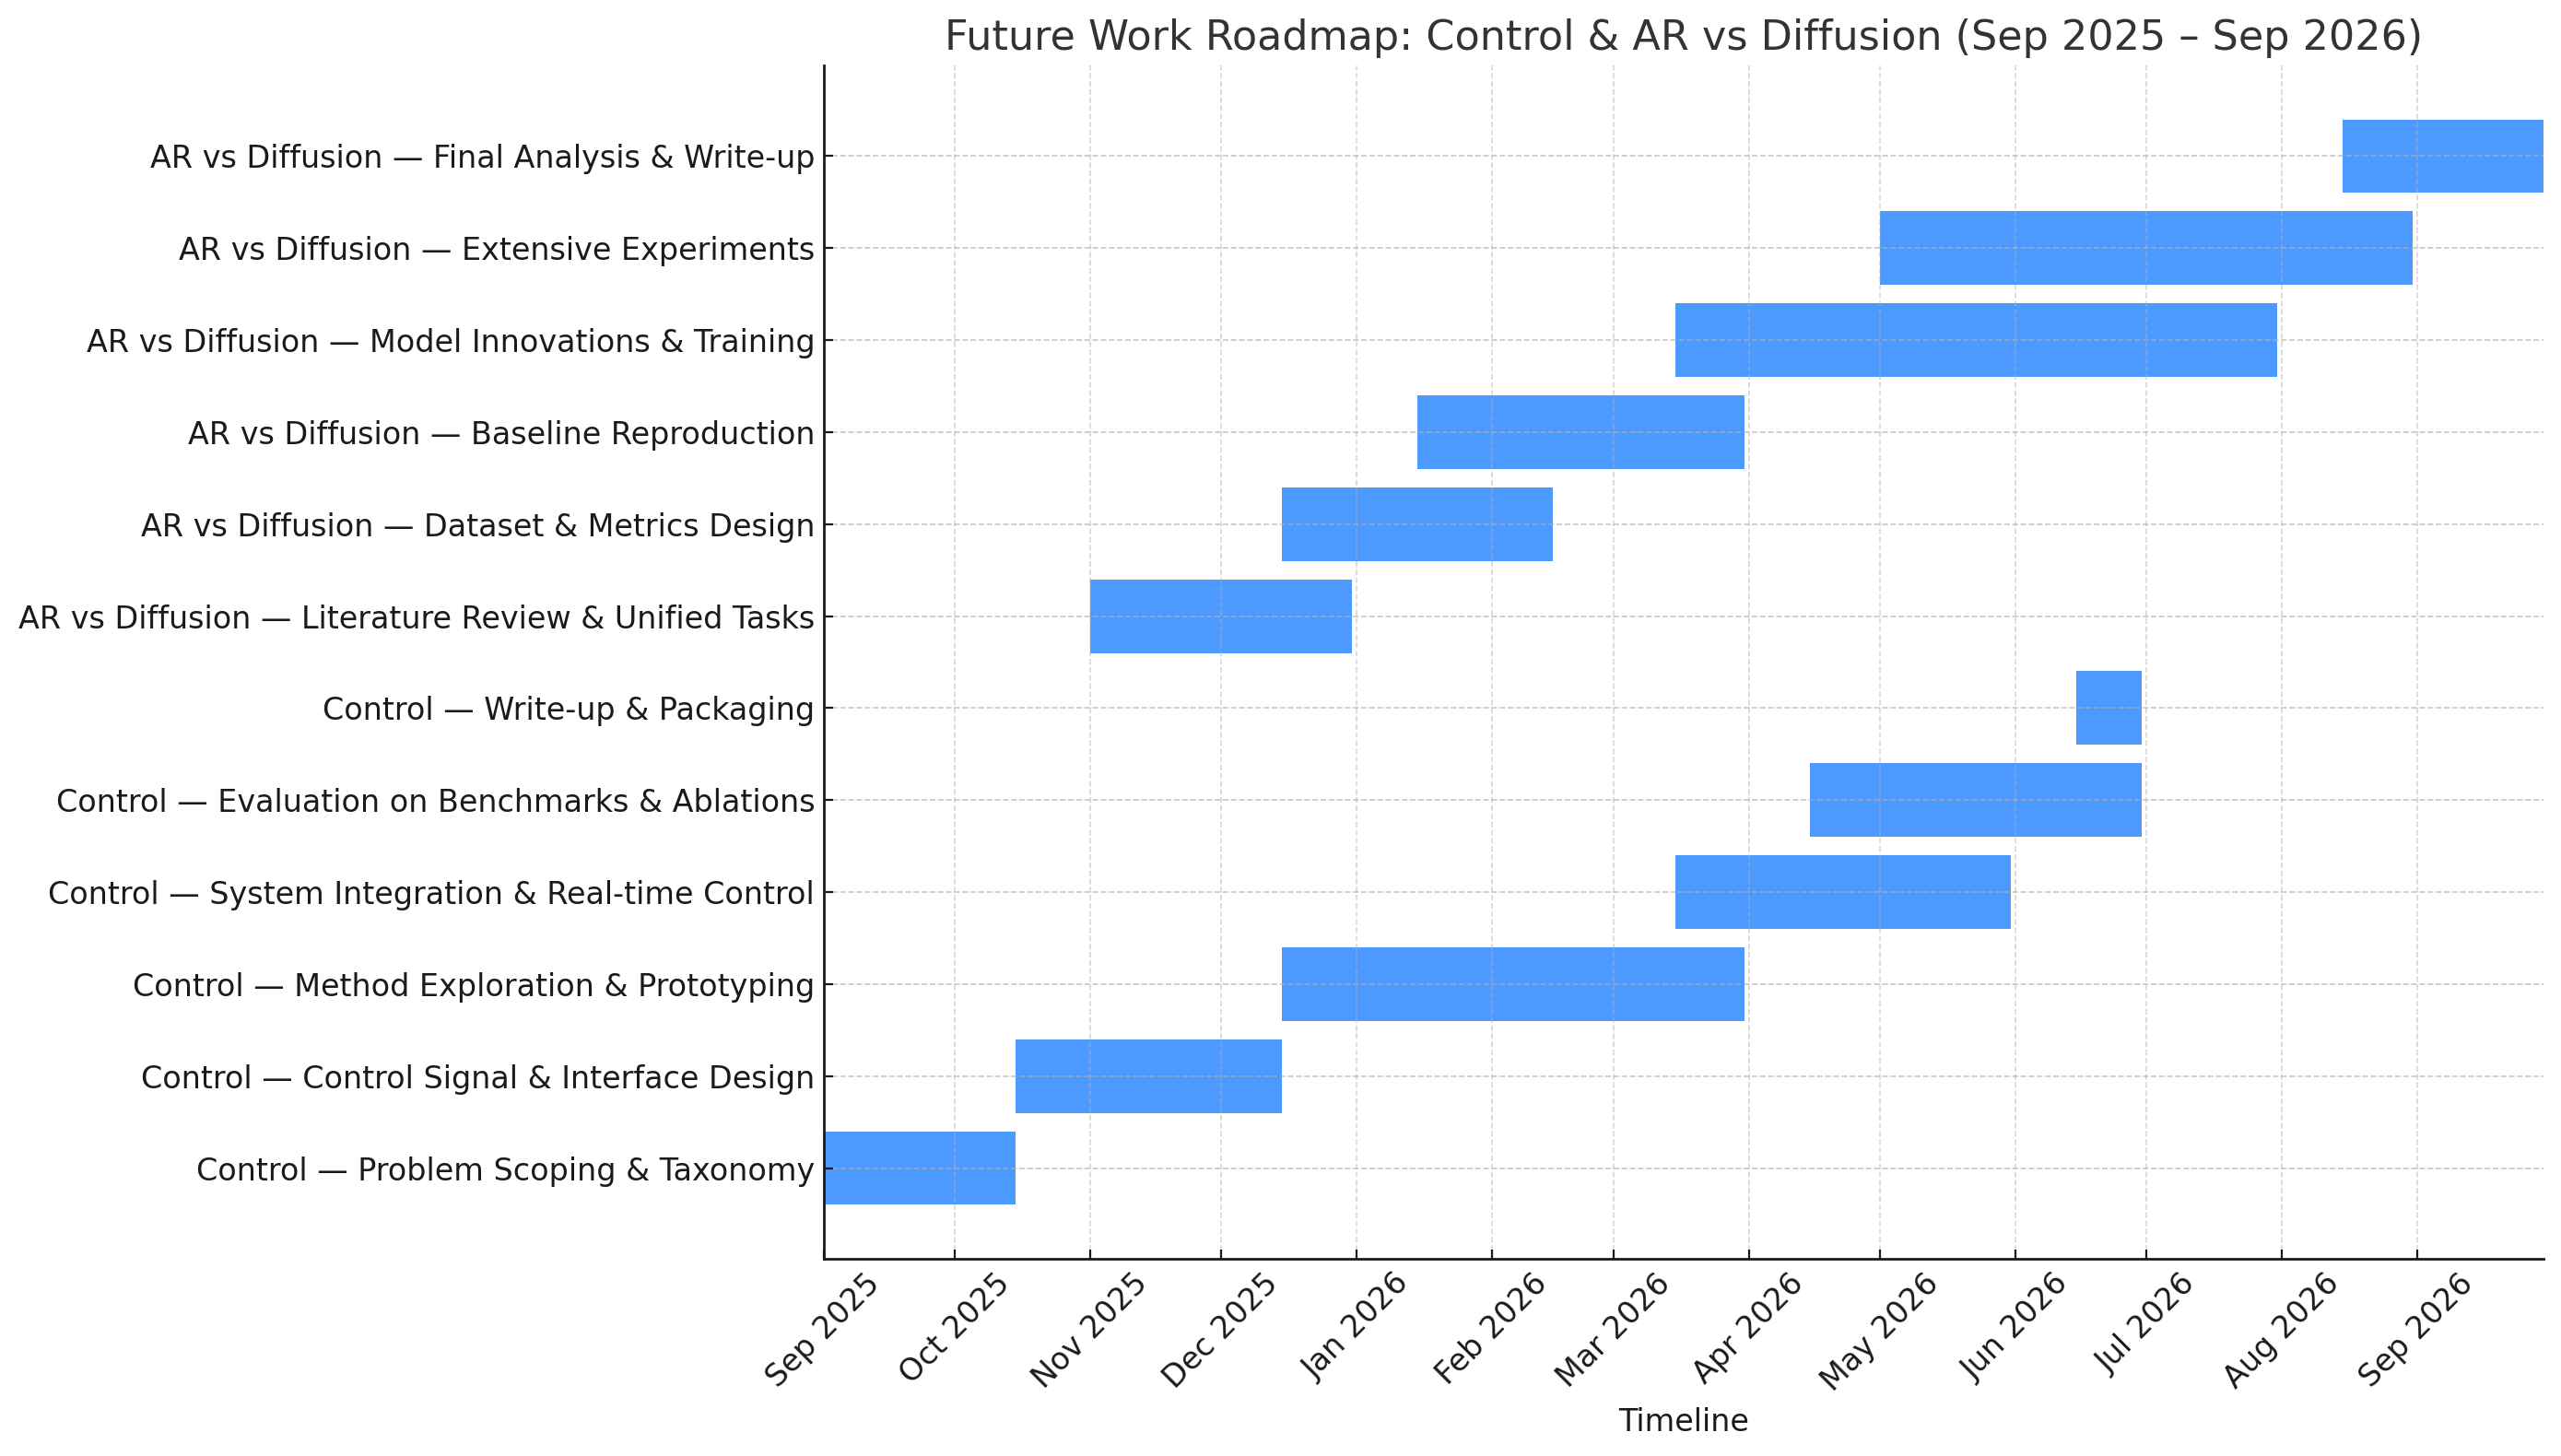
\includegraphics[width=1\textwidth]{gantt_two_projects_2025_09_to_2026_09_single_color.png}
    \caption{Planned research timeline and milestones spanning Sep.~2025 to Sep.~2026}
    \label{fig:gantt} 
\end{figure*}

\textbf{Overall aim.} 
my PhD research is designed to establish a unified, controllable, and efficient motion generation framework that advances both fundamental understanding and practical applications. The long-term trajectory is as follows:

\begin{itemize}
    \item \textbf{Year 2 (2025--2026): Scaling and generalization.} Extend the unified AR+diffusion framework to multi-dataset, multi-lingual, and multi-modal settings (e.g., audio, video, haptics). Investigate transfer learning and domain adaptation so that the model generalizes to unseen datasets and diverse human activities.
    \item \textbf{Year 3 (2026--2027): Applications and robustness.} Move from controlled benchmarks to open-world and real-time scenarios. Explore deployment in interactive systems (e.g., AR/VR, animation pipelines, human–robot interaction) with emphasis on latency, robustness under noisy inputs, and user-controllability.
    \item \textbf{Final goal (by graduation).} Deliver a controllable motion generation system that is (i) \emph{interpretable} (latent factors aligned with human-understandable controls), (ii) \emph{scalable} (handling long-horizon, multi-agent, and multimodal conditions), and (iii) \emph{deployable} (integrated into real-world applications with a balance between quality and efficiency). The outcome will be a comprehensive thesis and a suite of open-source tools, datasets, and reproducible benchmarks that contribute lasting value to the community.  
\end{itemize}


The next 12 months focus on two interconnected directions:  
(i) extending discrete and masked diffusion into an autoregressive (AR) formulation for efficient and controllable motion generation, and  
(ii) developing interpretable controllability via trajectory encoders and body-part/chain-wise VAEs, enabling consistent injection of control inputs such as joint trajectories, keyframes, or partial skeletons.  

\paragraph{September--December 2025: Baselines and unified control interface.}  
\begin{itemize}
    \item \textbf{Objective:} Establish a discrete diffusion baseline (masked-token and inpainting schemes) and design a unified control interface covering text and joint trajectories.  
    \item \textbf{Motivation:} Establish a solid, reproducible experimental framework so that subsequent studies can be conducted systematically with fair comparisons and minimal confounding factors. 
    \item \textbf{Tasks:}
    \begin{enumerate}
        \item Implement discrete diffusion with masking and classifier-free guidance.  
        \item Build reproducible evaluation pipelines with metrics including FID, R-Precision, MM-Dist, Diversity, MModality, etc..  
    \end{enumerate}
\end{itemize}

\paragraph{January--March 2026: From masked diffusion to autoregressive modeling.}  
\begin{itemize}
    \item \textbf{Objective:} Transfer control mechanisms from discrete diffusion to an AR model that combines block-based discrete representations with causal decoding.  
    \item \textbf{Motivation:} This enables retaining the strong controllability of diffusion while gaining the efficiency and streaming capability of autoregressive models.  
    \item \textbf{Tasks:}
    \begin{enumerate}
        \item Train AR models with discrete blocks as priors, aligned to text or trajectory conditions.  
        \item Investigate fusion strategies such as residual injection, cross-attention, and gated adapters.  
    \end{enumerate}
\end{itemize}

\paragraph{April--June 2026: Controllability via trajectory and part-wise VAEs.}  
\begin{itemize}
    \item \textbf{Objective:} Train interpretable encoders where latent variables are tied to anatomical parts or motion chains, enabling fine-grained control.  
    \item \textbf{Motivation:} Current models often treat the body holistically, which makes it difficult to constrain specific joints. By dividing into chains (e.g., arm, leg, spine), trajectories can be explicitly controlled while preserving global coherence.  
    \item \textbf{Tasks:}
    \begin{enumerate}
        \item Pre-train trajectory and part-wise VAEs with reconstruction or auxiliary tasks before integration into the main generator.  
        \item Design adapter-based fusion: apply trajectory hints and inject them via cross-attention with gated residuals, avoiding mismatches between complete trajectory hints and autoregressive generation.  
    \end{enumerate}
\end{itemize}

\paragraph{July--September 2026: Integration, evaluation, and final write-up.}  
\begin{itemize}
    \item \textbf{Objective:} Consolidate the AR and diffusion pipelines into a unified system with runtime controllability.  
    \item \textbf{Tasks:}
    \begin{enumerate}
        \item Conduct large-scale evaluations on HumanML3D, KIT-ML, and CMP, including zero/few-shot tasks and long-horizon sequences.  
        \item Package the system so that the same control interface can switch between diffusion and AR backends depending on latency/quality trade-offs.  
        \item Finalize thesis chapters and prepare journal submissions with comprehensive ablation studies and failure case analyses.  
    \end{enumerate}
\end{itemize}

\paragraph{Evaluation protocol.}  
Across all phases, evaluations will cover:  
\begin{itemize}
    \item \textbf{Distribution \& matching:} FID, R-Precision@k, MM-Dist, Diversity, MModality, MEC.  
    \item \textbf{Control quality:} joint trajectory error, keyframe accuracy, velocity/foot-contact consistency.  
    \item \textbf{Efficiency:} latency per step, throughput for streaming.  
\end{itemize}



All experiments will be released as config-driven scripts with fixed seeds to ensure reproducibility.

% \paragraph{Long-term vision and final goal.}  
% my PhD research is designed to establish a unified, controllable, and efficient motion generation framework that advances both fundamental understanding and practical applications. The long-term trajectory is as follows:

% \begin{itemize}
%     \item \textbf{Year 2 (2026--2027): Scaling and generalization.} Extend the unified AR+diffusion framework to multi-dataset, multi-lingual, and multi-modal settings (e.g., audio, video, haptics). Investigate transfer learning and domain adaptation so that the model generalizes to unseen datasets and diverse human activities.
%     \item \textbf{Year 3 (2027--2028): Applications and robustness.} Move from controlled benchmarks to open-world and real-time scenarios. Explore deployment in interactive systems (e.g., AR/VR, animation pipelines, human–robot interaction) with emphasis on latency, robustness under noisy inputs, and user-controllability.
%     \item \textbf{Final goal (by graduation).} Deliver a controllable motion generation system that is (i) \emph{interpretable} (latent factors aligned with human-understandable controls), (ii) \emph{scalable} (handling long-horizon, multi-agent, and multimodal conditions), and (iii) \emph{deployable} (integrated into real-world applications with a balance between quality and efficiency). The outcome will be a comprehensive thesis and a suite of open-source tools, datasets, and reproducible benchmarks that contribute lasting value to the community.  
% \end{itemize}



% TODO：如需要，添加甘特图与季度里程碑（数据/模型/评测/开源）。

% =========================================================
% Acknowledgements (optional)
% =========================================================
% \section*{Acknowledgements}
% TODO：资助与合作致谢（可选）。

% =========================================================
% References
% =========================================================
\bibliographystyle{plain}
\bibliography{references} % TODO：沿用既有 .bib

% =========================================================
% Appendices
% =========================================================
\appendix
% \section{Extended Metrics and Dataset Details}
% TODO：指标定义、数据统计与可视化、清洗流程与阈值表、伪代码。
\section{Data preparation for MotionDirector}
\subsection{HumanML3D Visualization}
To achieve visualization and in-depth analysis of the HumanML3D dataset, we first converted the .npy files into Biovision Hierarchy (BVH) format for convenient visualization using Blender software. However, skeletal-based virtual human motions often lack realism. Therefore, we further converted the BVH-format data into SMPL model format and applied skinning to enhance the visual authenticity of the motion.

Notably, the BVH format utilizes a skeletal structure comprising 17 joints, whereas the SMPL model includes 22 joints. The five additional joints in the SMPL model correspond to vertices at the extremities of the limbs and the top of the head. During conversion, to ensure compatibility, the values for these additional joints were set to zero. After generating the SMPL models, we assigned skinning weights and standardized the initial human shape to an A-pose to maintain consistency and standardization.

\begin{figure}[htbp]
    \centering
    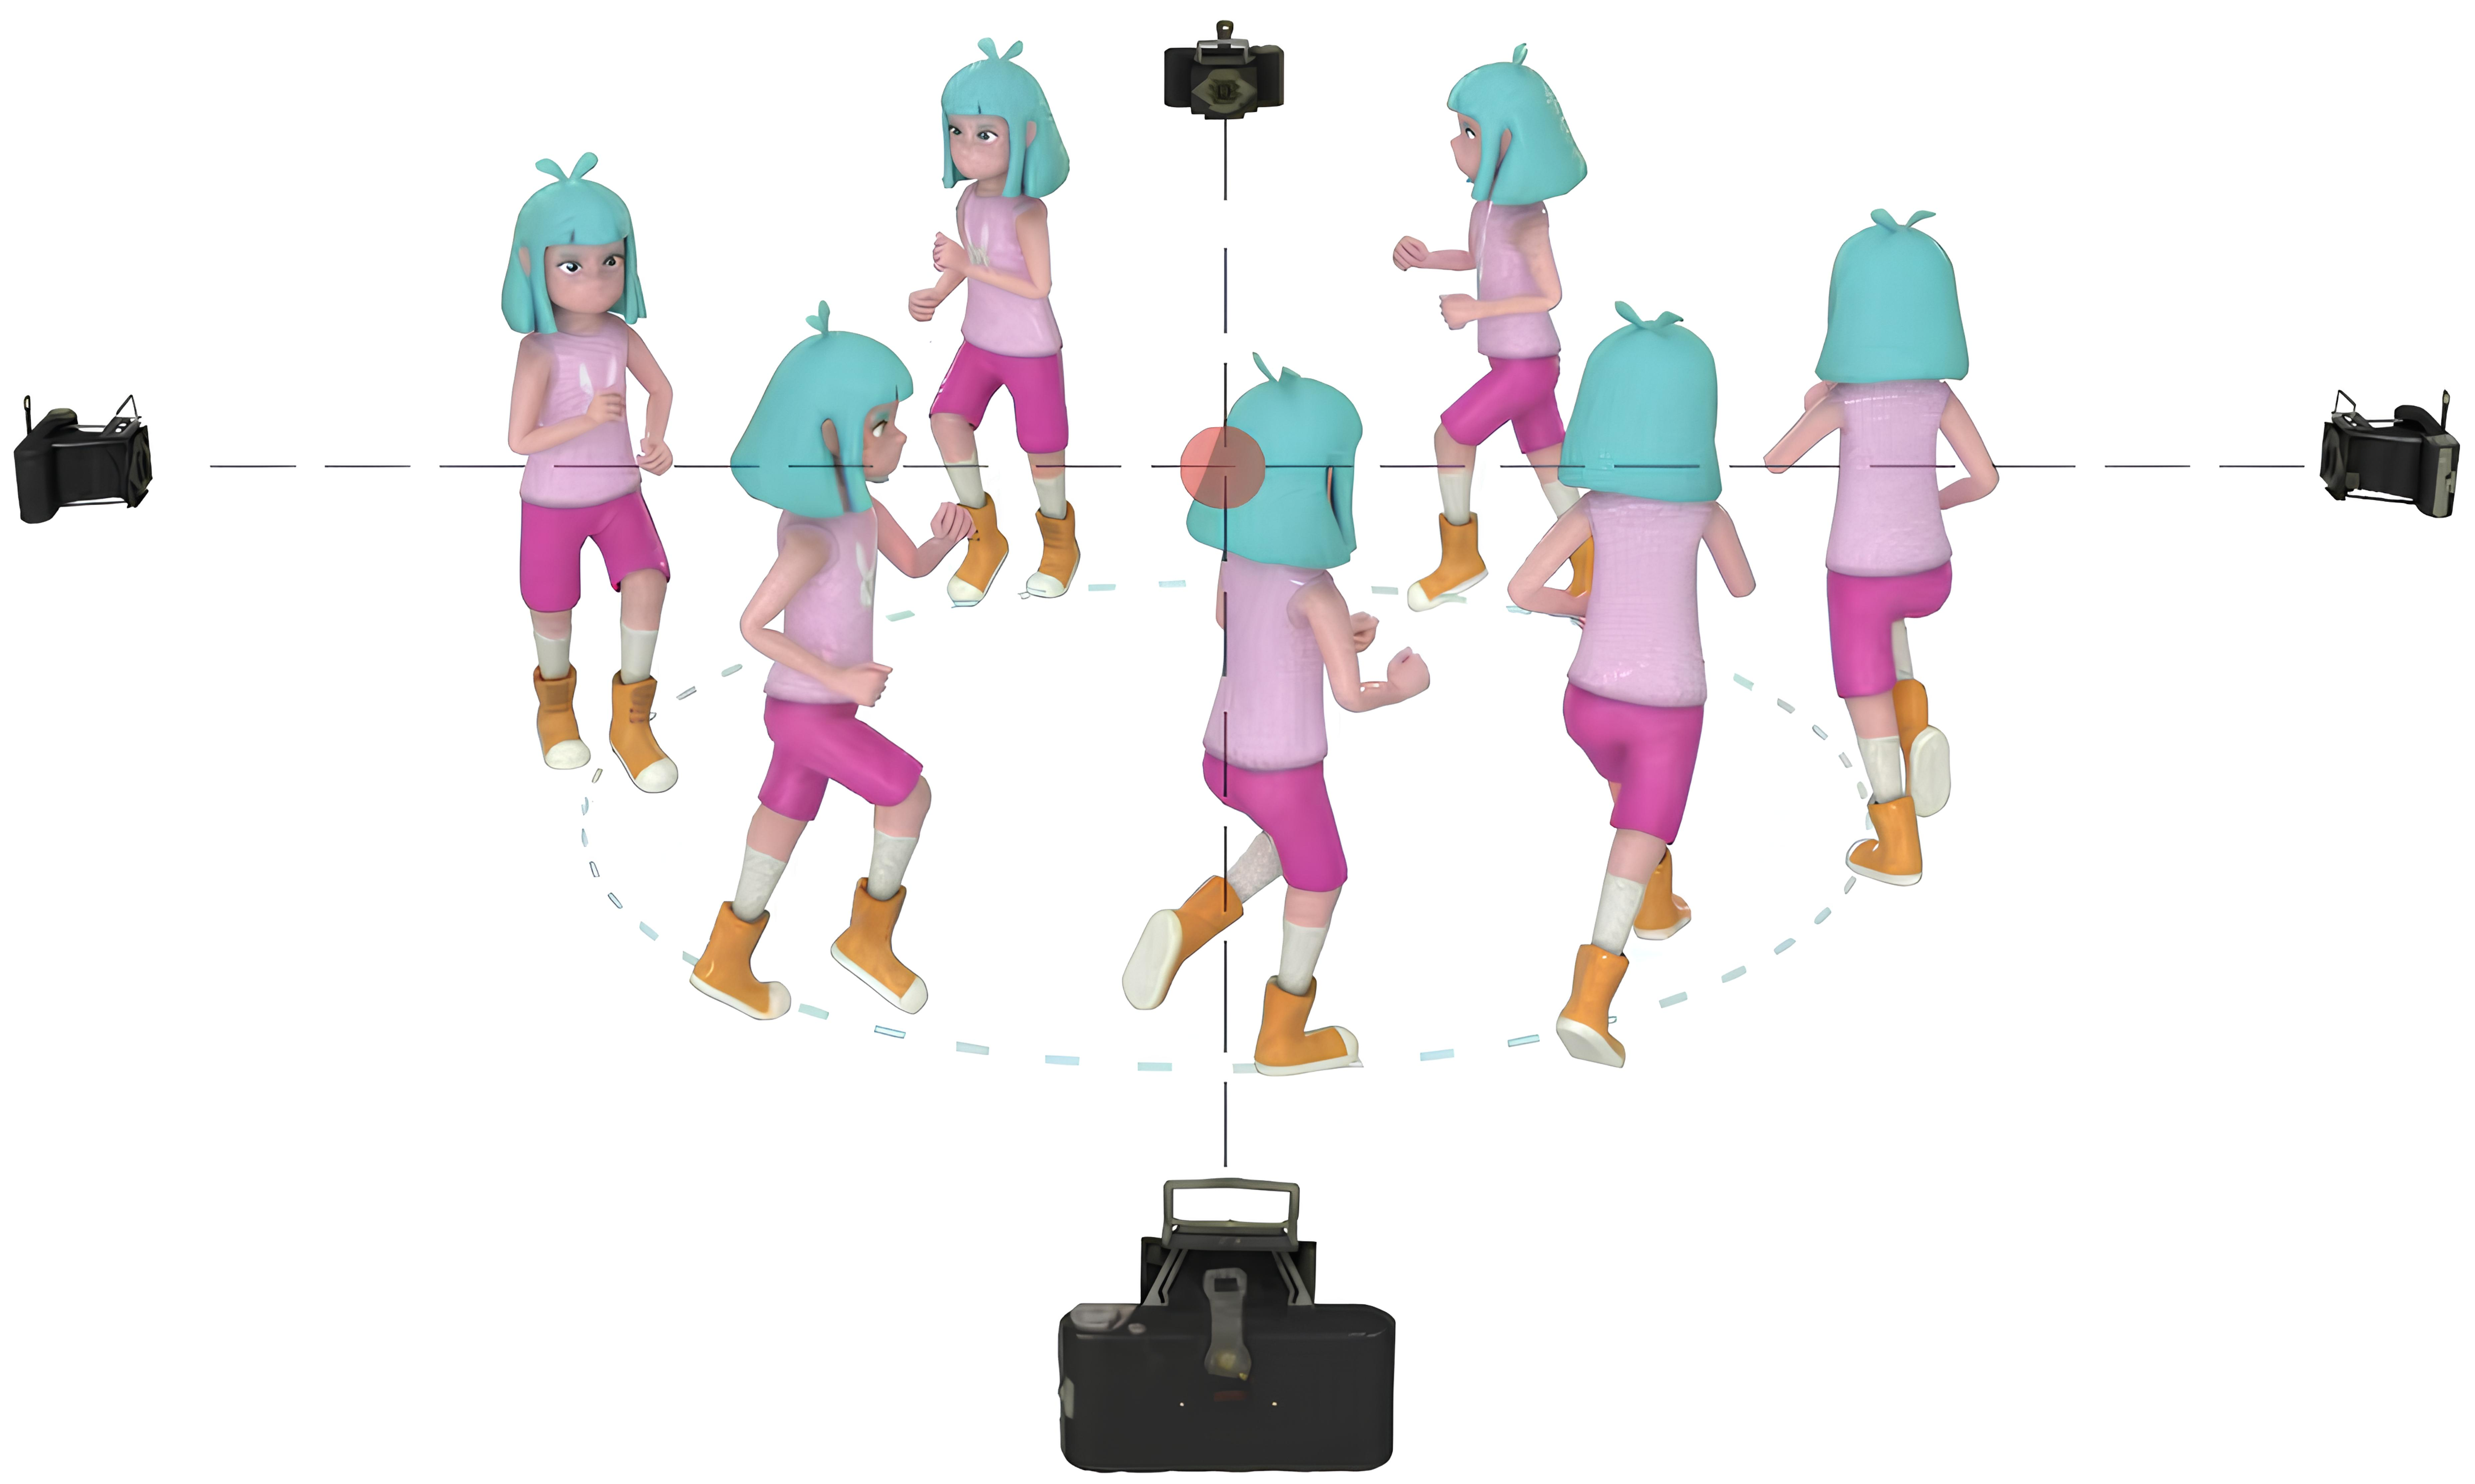
\includegraphics[width=0.7\linewidth]{fig_motion_Director/1.jpg}
    \caption{Video motion dataset creation workflow visualization.}
    \label{fig:Video motion dataset creation workflow visualization.}
\end{figure}

Subsequently, we converted the SMPL-format data into FBX format and utilized Blender software to set up four virtual cameras, capturing the motion sequences comprehensively from the east, south, west, and north directions, see Fig.~\ref{fig:Video motion dataset creation workflow visualization.}. This process yielded a total of 116,800 video motion videos. To ensure high data quality, we employed the data cleaning approach described in Appendix \ref{filter_method}, ultimately obtaining 71,220 video motion videos with limited but inevitable errors, accounting for approximately 61\% of the original dataset.


\subsection{Anomaly Data Analysis}
Based on the analysis results, anomalous motion samples account for 39\% of the entire dataset. Through visualization analysis, we were able to identify these anomalous samples and began investigating the reasons behind such a high anomaly rate. We categorized the anomalous data into three main types:
\begin{itemize}
    \item \textbf{Skinning errors}, which result in incorrect or inverted skin deformations of the human body, as shown in Fig.~\ref{fig:img1};
    \item \textbf{Data quality issues}, where the overall motion appears generally normal but contains locally unbalanced or disproportionate movements, as shown in Fig.~\ref{fig:img2};
    \item \textbf{Mild deviations in the motion itself}, where the motion sequence displays subtle but noticeable unnatural or unrealistic elements, as shown in Fig.~\ref{fig:img3}.

\end{itemize}
In the future, we plan to further improve our visualization methods by integrating more advanced techniques to gain a deeper understanding of and better monitor the quality of motion generation. These enhancements will help us identify deficiencies in the data creation process and guide the refinement of both generation and curation pipelines. Ultimately, this will facilitate the production of higher-quality motion samples.
\begin{figure}[t]
    \centering
    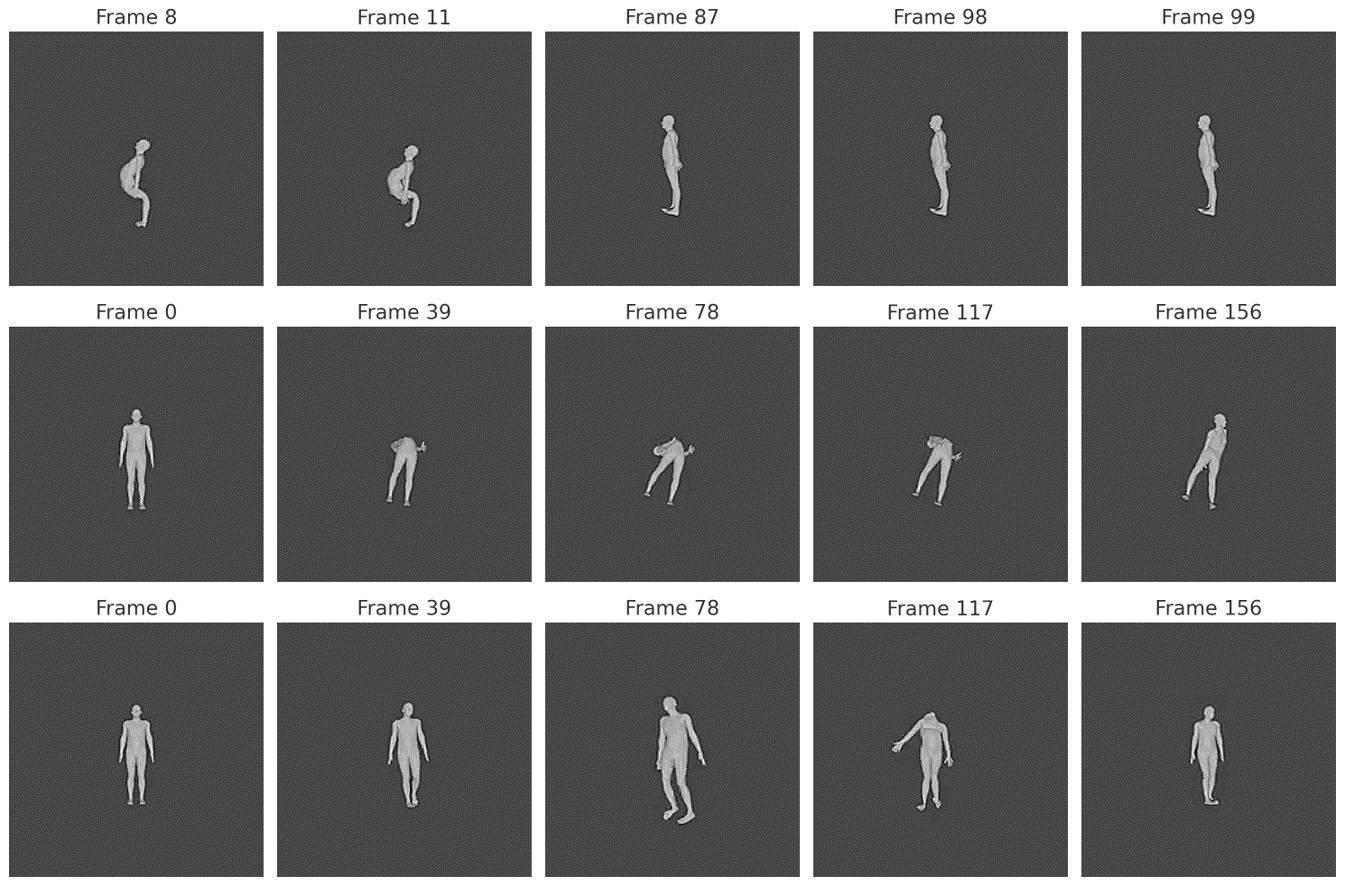
\includegraphics[width=0.8\textwidth]{fig_motion_Director/图片1.png}
    \caption{Skinning errors.}
    \label{fig:img1}
\end{figure}

\begin{figure}[t]
    \centering
    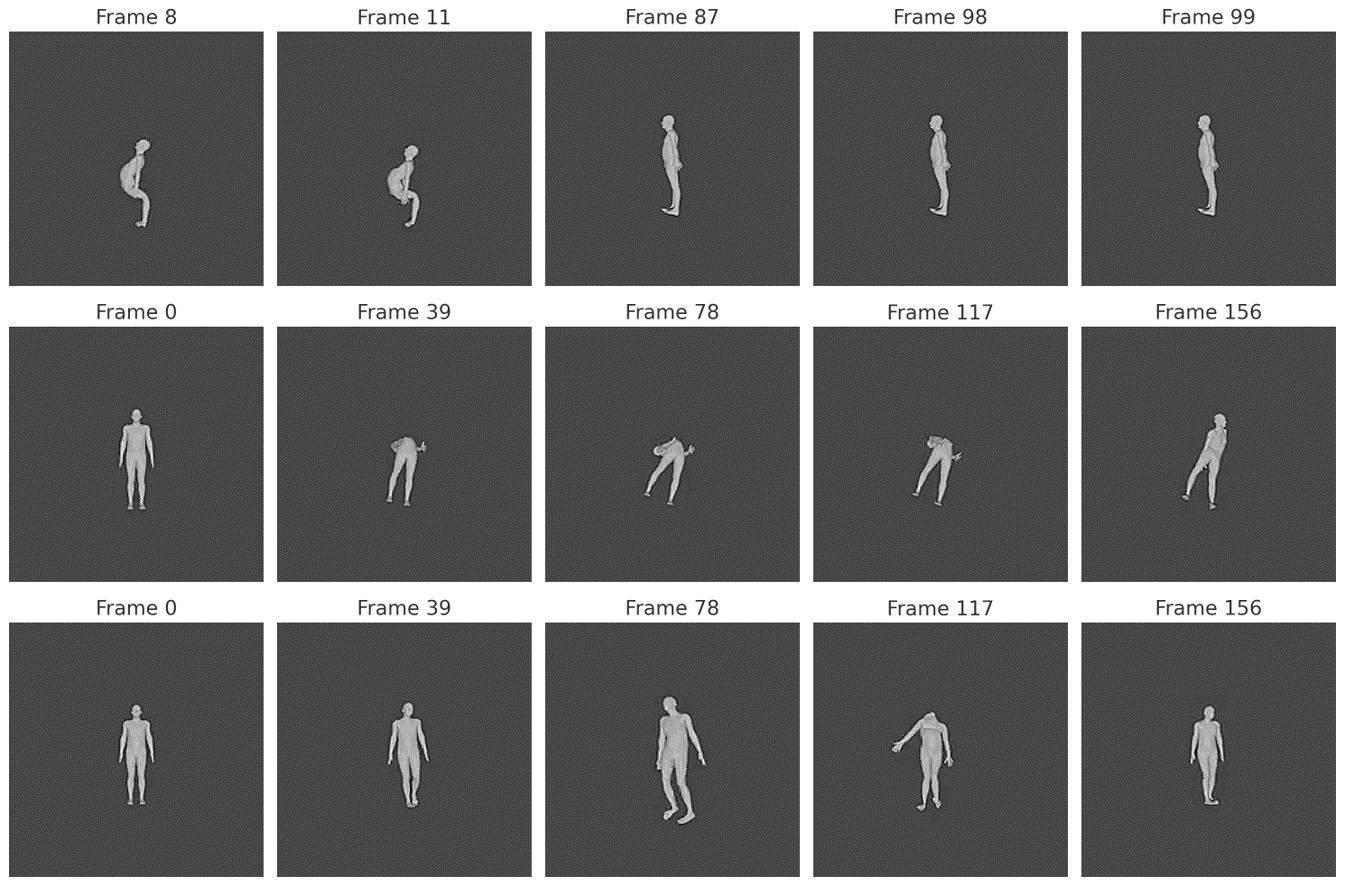
\includegraphics[width=0.8\textwidth]{fig_motion_Director/图片1.png}
    \caption{Data quality issues.}
    \label{fig:img2}
\end{figure}

\begin{figure}[htb]
    \centering
    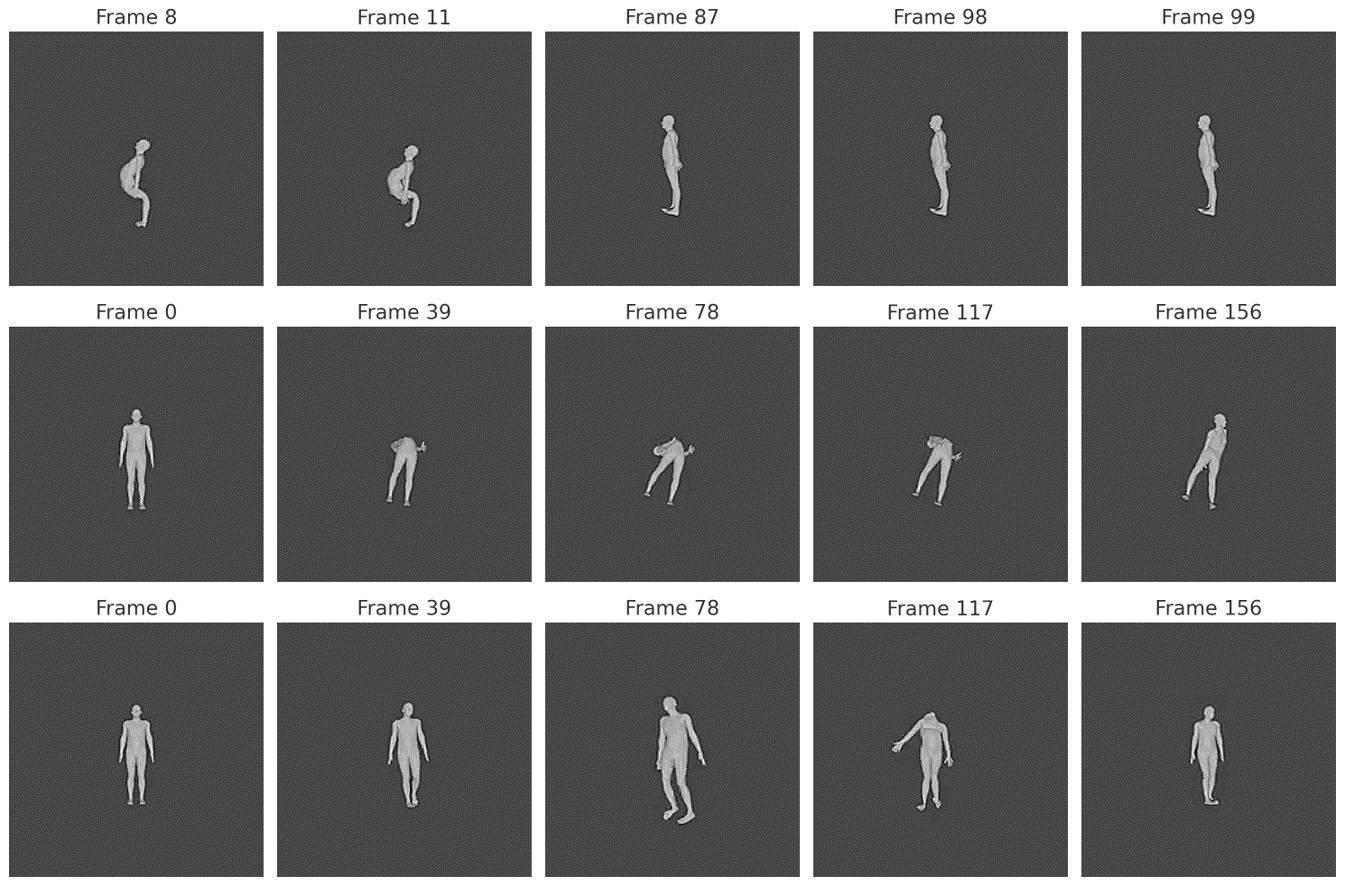
\includegraphics[width=0.8\textwidth]{fig_motion_Director/图片1.png}
    \caption{Mild deviations in the motion itself.}
    \label{fig:img3}
\end{figure}

\subsection{Automated Video Data Cleaning}
\label{Automated Video Data Cleaning}
To ensure high-quality data input for downstream motion analysis tasks, we implement a robust data cleaning algorithm that filters out erroneous or low-quality video samples based on human body orientation consistency. The method utilizes pose landmarks extracted via MediaPipe and evaluates the subject's orientation through a series of geometric and kinematic criteria. The key components of the cleaning algorithm are outlined as follows:

Let a video sample $V = \{I_t\}_{t=1}^T$ consist of $T$ frames. For computational efficiency, we sample a fixed subset of frames $\mathcal{F} = \{ I_{t_i} \mid i = 1, 2, \dots, N \}$ where $N \ll T$ using a uniform sampling strategy. Each frame $I_{t_i}$ is processed by a pose estimator to extract a set of 3D landmarks $\mathbf{L}_{t_i} \in \mathbb{R}^{J \times 3}$, where $J$ is the number of body joints.

\paragraph{Back-Face Consistency:}
Let $\vec{v}_{\text{back}} = \mathbf{L}_{\text{RShoulder}} - \mathbf{L}_{\text{LShoulder}}$
and $\vec{v}_{\text{hip}} = \mathbf{L}_{\text{RHip}} - \mathbf{L}_{\text{LHip}}$.
The body orientation vector is defined as
\begin{equation}
\vec{v}_{\text{body}} = \frac{1}{2} (\vec{v}_{\text{back}} + \vec{v}_{\text{hip}}).
\end{equation}
%
We also define the face direction vector as
\begin{equation}
\vec{v}_{\text{face}} = \mathbf{L}_{\text{Nose}} - \mathbf{L}_{\text{MidShoulder}},
\end{equation}
where $\mathbf{L}_{\text{MidShoulder}} = \frac{1}{2} (\mathbf{L}_{\text{LShoulder}} + \mathbf{L}_{\text{RShoulder}})$.
The body-face angle $\theta_{\text{bf}}$ is computed as
\begin{equation}
\theta_{\text{bf}} = \arccos \left( \frac{\vec{v}_{\text{body}} \cdot \vec{v}_{\text{face}}}{\|\vec{v}_{\text{body}}\| \cdot \|\vec{v}_{\text{face}}\|} \right).
\end{equation}
%
A frame is valid if $\theta_{\text{bf}} \leq \theta_0$, where $\theta_0 = 20^\circ$.

\paragraph{Head Pose Constraint:}
Let $\vec{v}_{\text{head}} = \mathbf{L}_{\text{Nose}} - \mathbf{L}_{\text{MidShoulder}}$.
We constrain the head tilt angle $\theta_{\text{head}}$ against the vertical axis:
\begin{equation}
\theta_{\text{head}} = \arccos \left( \frac{\vec{v}_{\text{head}} \cdot \vec{e}_y}{\|\vec{v}_{\text{head}}\|} \right).
\end{equation}
%
A frame is valid if $\theta_{\text{head}} \leq \theta_1$, with $\theta_1 = 30^\circ$, and $\vec{e}_y$ is the global vertical axis.


\paragraph{Foot-Knee Direction Alignment:}

To ensure the plausibility of gait or standing postures, we constrain the angle between the hip-to-knee vector and the ankle-to-foot vector. For each leg side $s \in \{\text{Left}, \text{Right}\}$, we define the foot-knee angle as:

\begin{equation}
\theta_{\text{fk}}^{(s)} = \angle \left( \mathbf{L}_{\text{Hip}}^{(s)} - \mathbf{L}_{\text{Knee}}^{(s)},\ \mathbf{L}_{\text{Foot}}^{(s)} - \mathbf{L}_{\text{Ankle}}^{(s)} \right),
\end{equation}

where $\mathbf{L}_{\text{Hip}}^{(s)}$, $\mathbf{L}_{\text{Knee}}^{(s)}$, $\mathbf{L}_{\text{Ankle}}^{(s)}$, and $\mathbf{L}_{\text{Foot}}^{(s)}$ are the coordinates of the respective joints on side $s$.

The frame is considered \emph{valid} with respect to foot-knee alignment if:

\begin{equation}
\theta_{\text{fk}}^{(s)} \in [75^\circ,\ 180^\circ], \quad \forall s \in \{\text{Left}, \text{Right}\}
\end{equation}

This constraint effectively filters out frames exhibiting unnatural foot twisting or anatomical inconsistencies, which often arise from pose tracking failures or annotation noise.


\paragraph{Frame Validity and Video Filtering:}
\label{filter_method}
A frame $I_{t_i}$ is marked as \textit{valid} if it satisfies all of the following constraints:
(1) back-face consistency,
(2) head pose constraint, and
(3) foot-knee direction alignment.


Let $B_i$, $H_i$, and $F_i$ denote Boolean indicators (1 if satisfied, 0 otherwise) for these three conditions on frame $i$.
We define the overall video validity score as:

\begin{equation}
P(v) = \frac{1}{N} \sum_{i=1}^{N} \mathbb{I}(B_i \land H_i \land F_i)
\end{equation}
where $\mathbb{I}(\cdot)$ is the indicator function that returns $1$ if the logical expression inside is true and $0$ otherwise.


A video is considered valid if:

\begin{equation}
P(v) \geq \rho,
\end{equation}

where $\rho = 0.7$ is the minimum acceptable ratio of valid frames.

To construct the cleaned validation dataset, we apply this automated filtering process to all raw videos.
Each video is uniformly sampled into $N = 12$ frame, pose landmarks are extracted via MediaPipe, and only videos passing the threshold are retained.
This ensures that downstream models are trained on reliable, consistent human motion data, free from noisy or erroneous poses.


% % 结束语：该清洗流程仅作为工程性增强，避免视频噪声干扰；不改变方法论主体
% \section{Additional Qualitative Comparisons}
% % TODO：更多可视化：编辑前后、长序列、流式与换prompt等。

% \section{Hyperparameters and Reproducibility}
% % TODO：超参总表、随机种子、环境/库版本、训练/推理脚本摘要与复现清单。
\end{document}
